\documentclass[12pt]{report}
\usepackage[a4paper, margin=25mm]{geometry}
\usepackage{amssymb} 
\usepackage{graphicx}
\usepackage{setspace}
\usepackage{titlesec}
\usepackage{titling}
\usepackage{lmodern}
\usepackage{ifthen}
\usepackage{amsmath,psfrag,pstcol}
\usepackage{float}
\usepackage[font=small,labelfont=bf,width=0.9\linewidth,margin=0.5cm]{caption}
\setlength{\parindent}{15pt}
\setlength{\parskip}{7pt}
\usepackage{subcaption}
\usepackage{tikz}
\usepackage{multirow}
\usepackage{makecell}
\usepackage[colorlinks=true, linkcolor=blue, citecolor=blue, urlcolor=blue, linktoc=page]{hyperref}
\usepackage{bookmark}
\usepackage[table]{xcolor}
\usepackage[intoc]{nomencl}
\makenomenclature
\renewcommand{\nomgroup}[1]{%
    \ifthenelse{\equal{#1}{A}}{\item[\textbf{Symbols}]}{}%
    \ifthenelse{\equal{#1}{Z}}{\item[\textbf{Acronym/Abbreviation}]}{}%
}
\onehalfspacing
\graphicspath{{images/}}
\usepackage{etoolbox}
% Set single spacing for tables
\AtBeginEnvironment{table}{\singlespacing}

\makeatletter
% Define a flag that turns on when \appendix is used
\newif\ifinappendix
\pretocmd{\appendix}{\inappendixtrue}{}{}
\makeatother

\usepackage{titlesec}
% Custom chapter formatting
\titleformat{\chapter}[display]
  {\normalfont\huge\bfseries}
  {\ifinappendix Appendix \thechapter \else \chaptername\ \thechapter \fi}
  {20pt}
  {
    \vspace*{-20pt}
  }

% Control spacing before/after chapter title block
\titlespacing*{\chapter}{0pt}{-30pt}{20pt}

\begin{document}

\pagenumbering{roman}
\begin{titlepage}
    \begin{center}
        \vspace*{1.5cm}

        
\includegraphics[width=0.25\textwidth]{University_Crest.pdf}\par
        \vspace{1cm}

        {\LARGE \textbf{Bias and Fairness in Automatic Spoken Language Assessment} \par}
        \vspace{1.5cm}

        \onehalfspacing
        Submitted June 2025, in fulfillment of \\
        the conditions for the award of the degree \textbf{Master of Engineering}.
        \vspace{1cm}

        \normalsize
        \textbf{Chloe Yee Man Yiu} \\
        Lucy Cavendish College
        \vspace{1cm}

        \textbf{Supervised by Dr Kate Knill}
        \vspace{1cm}

        Department of Engineering \\
        University of Cambridge
    \end{center}
\end{titlepage}

\section*{\centering Declaration}
\vspace{1.5cm}
\begin{flushleft}
I hereby declare that, except where explicit reference is made to the work of others, the content of this report is my own and has not been submitted, in whole or in part, for assessment towards any other qualification at any institution. All work contained herein was completed by me unless otherwise stated in the text or acknowledged appropriately. This report does not exceed 50 pages, including the main text, footnotes, tables, figures, appendices, and bibliography.
\end{flushleft}

\vspace{1.5cm}
\begin{flushright}
    \textbf{Chloe Yee Man Yiu}\\
    June 2025
\end{flushright}
\clearpage

\section*{\centering Acknowledgements}
\vspace{1.5cm}
\begin{flushleft}
I am sincerely thankful to my supervisor, Dr Kate Knill, for her consistent support and guidance throughout the year in shaping my project and helping me produce results that extend beyond academic curiosity. Her insightful feedback and regular meetings were key to the success of this work.

Thanks to Cambridge English Language Assessment, for support and access to data and resources. I also appreciate the helpful discussions and advice from members of the ALTA Speech Team.

Finally, I express my gratitude to my family and friends for their unwavering support and encouragement throughout my time at University of Cambridge, making this journey both enjoyable and fulfilling.
\end{flushleft}
\clearpage

\begin{center}
    \Large
    \textbf{Bias and Fairness in Automatic Spoken Language Assessment}
    \vspace{0.2in} \\

    \normalsize
    \textbf{Chloe Yee Man Yiu} \\
    Lucy Cavendish College \\
    Supervised by Dr Kate Knill
    \vspace{0.1in}

    June 2025
\end{center}

\section*{Technical Abstract}

Hola como estas here is for the abstract.

Could I use the one Mengjie wrote for the UKSI application?

\clearpage


\tableofcontents
\clearpage

% \addcontentsline{toc}{chapter}{List of Tables}
% \listoftables
% \clearpage

% \addcontentsline{toc}{chapter}{List of Figures}
% \listoffigures
% \clearpage

% \addcontentsline{toc}{chapter}{Nomenclature}
{\fontsize{11}{11}\selectfont
  \printnomenclature
  \clearpage}

\pagenumbering{arabic}

\chapter{Introduction}

\section{Motivation}
In recent years, English has been more commonly the preferred language of communications in many setting. The assessment of spoken English has therefore become increasingly important, especially in the context of education and employment opportunities. Traditionally, human examiners have been used to evaluate spoken English, but this approach is time-consuming and subjective. As a result, there has been a growing interest in developing automated systems for spoken language assessment.

Multiple systems have been developed to examine the spoken language proficiency of candidates. Three commonly investigated systems are text-based, feature-based, and speech-based systems \cite{graders}. Each type of model has its own method of processing the input speech and generating the intermediate vector $\mathbf{\hat{x}}$ (Chapter \ref{chap:graders}), which encapsulates information about the speech. Vector $\mathbf{\hat{x}}$ is passed into different neural network graders to produce the final score. The scoring process within the neural network is hard to be interpreted, causing non-transparency in the grading process. Problems such as potential biases within the system may then go undetected.

\begin{figure}[H]
    \centering
    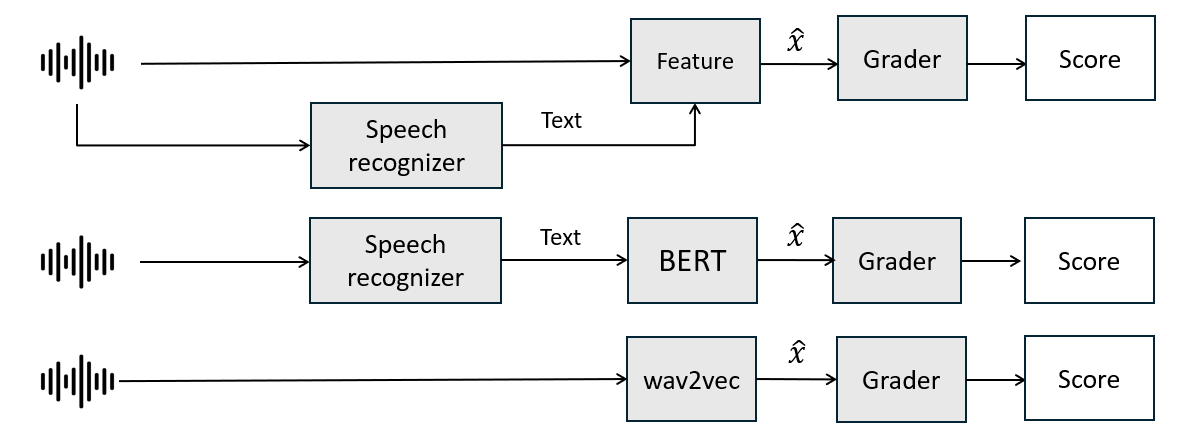
\includegraphics[width=0.7\textwidth]{grader.png}
    \caption{Spoken language assessment system for determining scores under consideration}
    \label{grader}
\end{figure}

A grader is unbiased if it evaluates speech samples solely based on performance-related factors, such as vocabulary richness and fluency, without being influenced by irrelevant attributes like gender, age and first language. It is important to ensure that the grading process is fair for candidates of all background, as unfair evaluations could have serious consequences for candidates' academic and professional opportunities. However, biases have previously been detected in other language models. For example, as existing natural language processing (NLP) tool are mainly trained with standard American English, language identifier misclassifies more frequently when processing African-American English as other languages, leading to biased results \cite{bias}. It is reasonable to expect that similar biases may exist in the spoken language assessment systems, performing particularly poorly for specific groups of candidates. Hence, it is pivotal to develop rigorous methods to measure and mitigate bias in these systems.

\section{Previous Work}
Concept activation vector (CAV) \nomenclature[Z]{CAV}{Concept Activation Vector} has previously been used to measure bias in a feature-based deep density network (DDN) \nomenclature[Z]{DDN}{Deep Density Network} models \cite{feature_bias}. Features related to the audio (energy level) and fluency (silence duration, long silence duration, word number and frequency, phone duration) are extracted from the audio as the intermediate vector \cite{feature_vector_old}. The CAV is extracted from the neural network without using weighting. There are two methods for CAV to measure bias: gradient-based (Chapter \ref{chap:cav}) and feature-based distance. The previous work investigated both methods.

% The experiment involves candidate data from the Use of Business English test (BULATS), which involves an initial short answer section, a read-aloud section, and three more general free speaking prompt-response answers. The scores were averaged over all sections to yield a score in the range 0 to 6.

When CAV indicated the presence of bias, the model's performance for that group of candidates, measured by the root mean squared error (RMSE), \nomenclature[Z]{RMSE}{Root Mean Squared Error} may or may not be worse than the initial performance. However, when CAV indicated the absence of bias for a particular group of candidates, the model's performance for them are also as good as the overall performance. This mean the CAV might not be sufficient to indicate bias presence, but enough to indicate the absence of it.

\section{Approach}
While the previous focuses on feature-based model, there are other types of models, which takes in text and speech, rather than features, as the input. The performance of CAV on these types of models is not well understood. The work aims at extending the investigation of CAV to other types of models. The gradient distance method is focused on, and it is found that the models display different gradient distance pattern.

In addition, previous research did not take into account the imbalance of concepts in the dataset, which could affect the CAV performance. Dataset might have more negative concepts than positive concepts. For example, people with their first language (L1) \nomenclature[Z]{L1}{First Language} as Thai is far less than people having other L1. The CAV extraction would not try to weight the minority group higher. Hence, the effect of using balanced weighting in the CAV extraction process is explored. It is shown that despite a difference in CAV performance, the ability of measuring bias is not affected.

The different types of models differ in terms of the input they take, and the design of the neural network grader. The work therefore attempts to isolate the factors affecting the difference in bias measurement across the models. The input into the system is found to be the factor having the most significant impact on the gradient distance pattern.

\section{Report Outline}
This report consists of 6 chapters with the following structure:
\begin{itemize}
    \item Chapter \ref{chap:graders} describes the different types of graders which would have its fairness being measured.
    \item Chapter \ref{chap:cav} outlines the steps of CAV extraction.
    \item Chapter \ref{chap:setup} describes the construction of training, calibration and testing data, alongside explanation on model biasing, factor isolation setup, and justification of performance metrics and hyper-parameters.
    \item Chapter \ref{chap:results} presents the results of the experiment, and discusses the implications.
    \item Chapter \ref{chap:conclusions} concludes the report and discusses future work.
\end{itemize}
\chapter{Spoken Language Assessment} \label{chap:graders}

The three types of models under investigation are: text-based, feature-based, and audio-based models. Each grader has its own architecture, with different number of layers, neurons, activation functions, and dropout rates. The dropout rate is the proportion of neurons that are randomly set to zero during training, which helps prevent overfitting. Table \ref{activation functions} defines the types of activation functions under consideration, where $\alpha$ is a small constant ($<<1$) that allows a small gradient when the unit is not active.

\begin{table}[H]
    \centering
    \begin{tabular}{|c|c|}
        \hline
        \textbf{Activation Function}                                                             & \textbf{Definition}                     \\ \hline
        Rectified Linear Unit (ReLU) \nomenclature[Z]{ReLU}{Rectified Linear Unit}               & $f(x) = \max(0, x)$                     \\ \hline
        Leaky Rectified Linear Unit (LReLU) \nomenclature[Z]{LReLU}{Leaky Rectified Linear Unit} & $f(x) = \begin{cases}
                                                                                                                   x,        & \text{if } x > 0    \\
                                                                                                                   \alpha x, & \text{if } x \leq 0
                                                                                                               \end{cases}$ \\ \hline
    \end{tabular}
    \caption{Activation functions under consideration}
    \label{activation functions}
\end{table}

Each grader also have its own model type - it could be a deep neural network (DNN) \nomenclature[Z]{DNN}{Deep Neural Network} or a deep density network (DDN). A DNN directly outputs the score from the input vector, using mean squared error (MSE) \nomenclature[Z]{MSE}{Mean Squared Error} loss function. A DDN, on the other hand, predicts the score from the input vector using a Gaussian distribution, outputting the mean ($\mu$) \nomenclature[A]{$\mu$}{Mean} and the standard deviation ($\sigma$) \nomenclature[A]{$\sigma$}{Standard deviation}. It uses negative log-likelihood for multivariate Gaussian (NLL) \nomenclature[Z]{NLL}{Negative Log-Likelihood} loss function.

The formula for the MSE and NLL loss functions are given by:
\begin{equation} \label{eq:mse}
    \text{MSE} = \frac{1}{N} \sum_{i=1}^{N} (y_i - \hat{y}_i)^2
\end{equation}
\begin{equation} \label{eq:nll}
    \text{NLL} = -\frac{1}{N} \sum_{i=1}^{N} \left( \log(\sigma_i^2) + \frac{(y_i - \mu_i)^2}{(2\sigma_i^2 + \epsilon)} \right)
\end{equation}
where $N$ is the number of samples, $y_i$ is the true score,  $\hat{y}_i$ is the predicted score, and $\epsilon = 1\times10^{-8}$ is a small constant to prevent division by zero.

The result would then be passed through linear calibration with the output result shown in equation \ref{eq:calibration}. The calibration is done using a linear regression model, which is trained to minimize the MSE between the predicted and true score. The linear regression model outputs two parameters: the slope ($m$) \nomenclature[A]{$m$}{Slope} and the intercept ($c$) \nomenclature[A]{$c$}{Intercept}. The calibrated score is then calculated using the formula:

\begin{equation}
    \hat{y}_{\text{calibrated}} = m*\hat{y}_{\text{uncalibrated}} + c
    \label{eq:calibration}
\end{equation}

Each grader also has its own way to process the input data to the intermediate vector $\hat{x}$. The following sections describe the architecture of each model in detail.

\section{Text-based Model}
Figure \ref{fig:text} shows the architecture of the text-based model. The BERT processing begins with text transcript extracted by WHISPER automatic speech recognition (ASR) from the candidate's audio. Each sample is fed through the BERT tokenizer \nomenclature[Z]{BERT}{Bidirectional Encoder Representations from Transformers}, which converts the text into a sequence of independent tokens ($\mathcal{T}$). $\mathcal{T}$ is then passed through the BERT encoder, creating contextualized embeddings for the tokens ($\mathcal{C}$), which takes into account the surrounding tokens. $\mathcal{C}$ is further passed through four independent attention mechanisms. Their outputs, each of 768 dimensions, are concatenated to form the 3072-dimensional token embeddings $\hat{x}$.

The token embeddings $\hat{x}$ is then passed through a fully connected DNN with 2 hidden layers, using the ReLU activation function. Each layer is labelled with a red box, with the red number indicating the change in dimension after each layer. The output is a single scalar indicated the predicted score.

\begin{figure}[H]
    \centering
    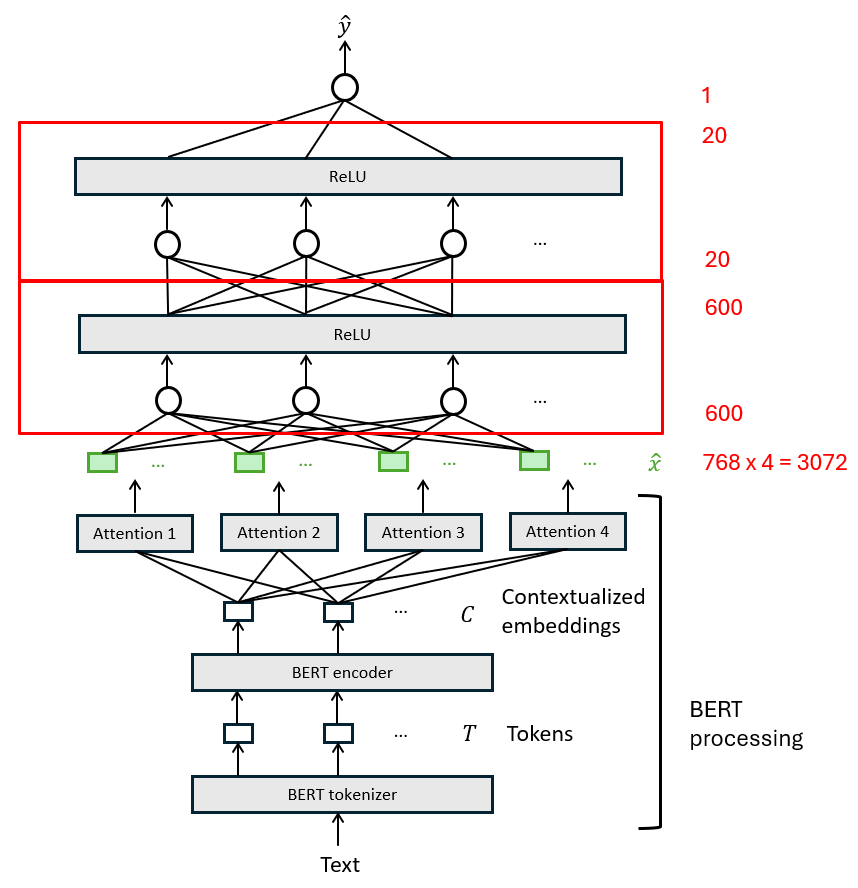
\includegraphics[width=0.7\textwidth]{text.png}
    \caption{Text-based model architecture}
    \label{fig:text}
\end{figure}

\section{Feature-based Model}
Figure \ref{fig:feature} shows the architecture of the feature-based model. The speech data have been extracted to produce a 356-dimensional vector using a custom extractor described in \cite{feature}. The features include statistics of: word level, phone duration, rhythm, fluency, and frequency \cite{graders}, with the full list of features detailed in \cite{feature}'s appendix.

The feature vector $\hat{x}$ is then passed through a fully connected DDN with 3 hidden layers. LReLU with $\alpha = 0.01$ is used as the activation function, and the dropout rate is set to 0.5. The output includes both $\mu$ and $\log(\sigma)$ of the predicted score Gaussian distribution. Similarly, the red box and red number indicated the layers and the dimension change.

\begin{figure}[H]
    \centering
    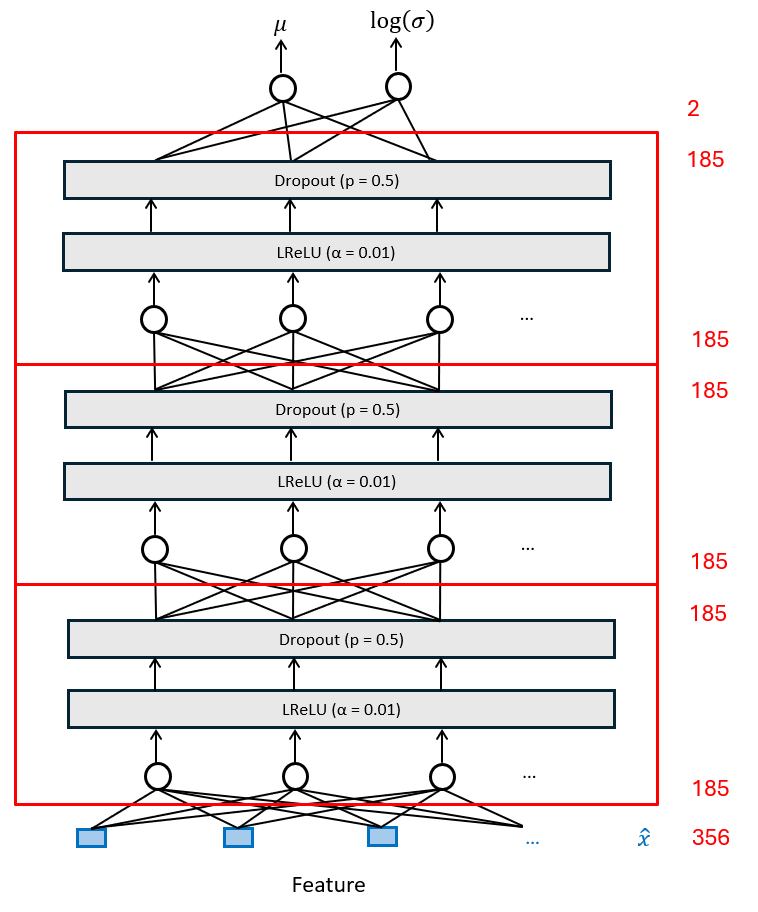
\includegraphics[width=0.7\textwidth]{feature.png}
    \caption{Feature-based model architecture}
    \label{fig:feature}
\end{figure}

\section{Audio-based Model}
Figure \ref{fig:audio} shows the architecture of the audio-based model. The wav2vec processing begins with the audio vector for each candidate described in \cite{graders}, which are 16kHz with duration 10-20 seconds. The data collator aggregates meta data (candidate number, attention masks), feeding vector to the wav2vec encoder, which creates contextualized embeddings for the tokens ($\mathcal{C}$). $\mathcal{C}$ is passed through two layers of 4 individual attention mechanisms. The output is concatenated to form the 3072-dimensional  token embeddings $\hat{x}$.

The token embeddings $\hat{x}$ is then passed through a fully connected DNN with a hidden layer, using the ReLU activation function and a dropout rate of 0.1. The output is a single scalar indicating the predicted score. As above, the red box and red number indicate the layers and the dimension change.

\begin{figure}[H]
    \centering
    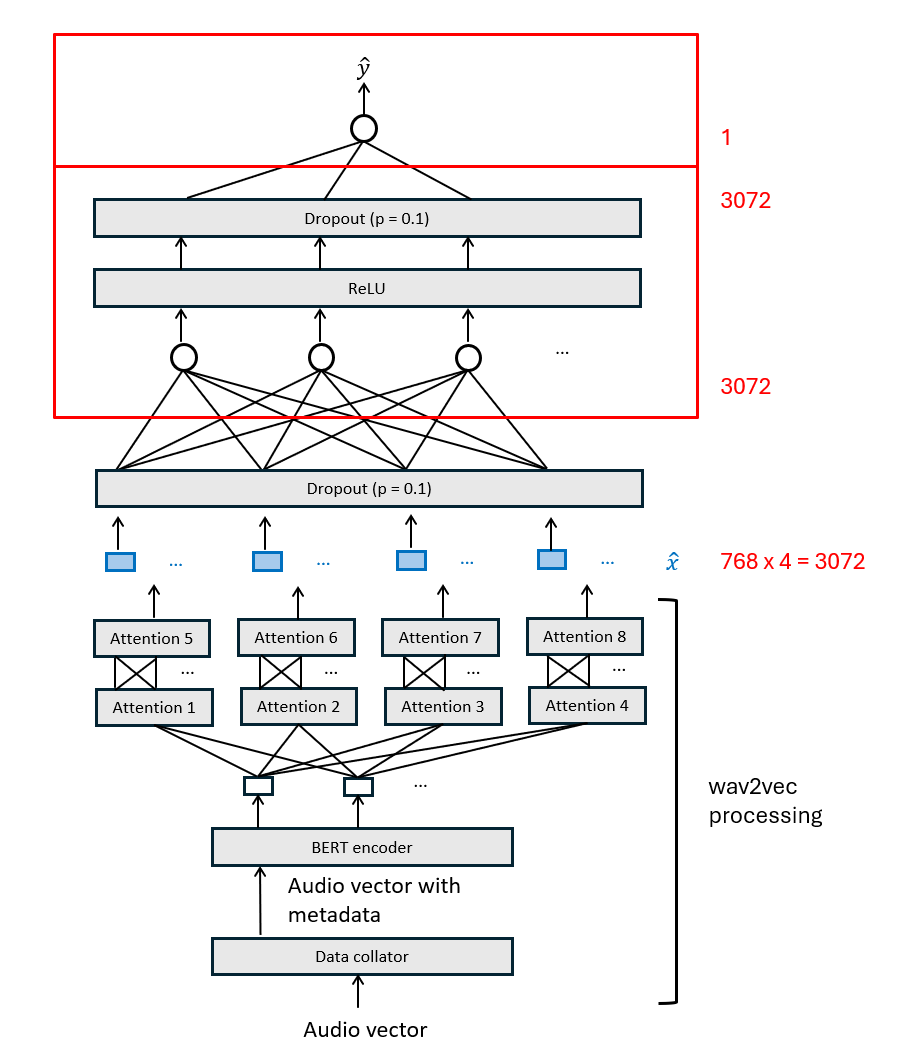
\includegraphics[width=0.7\textwidth]{audio.png}
    \caption{Audio-based model architecture}
    \label{fig:audio}
\end{figure}

\section{Summary}
This chapter describes the differences across the three types of models under investigation. Table \ref{tab:models} summarizes their key differences, including the input data, model type, activation function, dropout rate, and node numbers. Understanding these differences would be crucial for isolating factors that affect bias measurement.

\begin{table}[H]
    \centering
    \begin{tabular}{|c|c|c|c|}
        \hline
                                     & \textbf{Text-based}                                 & \textbf{Feature-based} & \textbf{Audio-based} \\ \hline
        \textbf{Intermediate Vector} & Text embeddings                                     & Feature vector         & Audio embeddings     \\ \hline
        \textbf{Model Type}          & DNN                                                 & DDN                    & DNN                  \\ \hline
        \textbf{Activation Function} & ReLU                                                & LReLU                  & ReLU                 \\ \hline
        \textbf{Dropout Rate}        & /                                                   & 0.5                    & 0.1                  \\ \hline
        \textbf{Node Numbers}        & $3072 \rightarrow 600 \rightarrow 20 \rightarrow 1$
                                     & \makecell[l]{
        $356 \rightarrow 185 \rightarrow$                                                                                                  \\
            $185 \rightarrow 185 \rightarrow 2$
        }
                                     & $3072 \rightarrow 3072 \rightarrow 1$                                                               \\ \hline
    \end{tabular}
    \caption{Summary of the three types of models under investigation}
    \label{tab:models}
\end{table}

\chapter{Concept Activation Vector Method} \label{chap:cav}

\section{Introduction}
The Concept Activation Vector (CAV) method is a technique to learn meaningful directions from the hidden layers of a neural network \cite{cav_def}.Test with Concept Activation Vectors (TCAV) \nomenclature[Z]{TCAV}{Test with Concept Activation Vectors} was proposed to measure how sensitive a neural network is to a human-defined concept \cite{tcav}. For example, given a classifier that predicts whether an image contains zebra, a CAV with the concept `stripes' could be used to measure how important stripes are to the classifier's decision.

Xizi worked on using CAV to measure bias within a feature-based DDN grading system \cite{feature_bias}, which is built on the fact that the CAV method could measure bias. The research in \cite{tcav} has identified positive linkage of the concept `female' with the classification of `aprons', which shows a gender bias over objects. Hence, it is proposed that CAV could also measure whether these human concepts would affect the grading process of the models.

The rest of this chapter would discuss the concept of CAV - how it is extracted from the models, and how it is used to measure bias.

\section{Extraction of CAV} \label{sec:cav_extraction}
When training the models in chapter \ref{chap:graders}, a supervised training data ($\mathcal{D}$) with intermediate vector $\mathbf{\hat{x}}^{(i)}$ and the true score $y^{(i)}$. The neural network ($\mathcal{F}$) is trained with $\mathbf{\hat{x}}^{(i)}$ and the network parameters $\boldsymbol{\theta}$. For DNN, $\mathcal{F}$ outputs the predicted score $\hat{y}^{(i)}$ in equation \ref{eq:DNN}. For DDN, $\mathcal{F}$ outputs the predicted Gaussian distribution with mean $\mu^{(i)}$ and standard deviation $\sigma^{(i)}$ in equation \ref{eq:DDN}.

\begin{equation} \label{eq:DNN}
    \mathcal{D} = \left\{\{\mathbf{\hat{x}}^{(i)},y^{(i)}\}\right\}_{i=1}^{N}; \qquad \mathbf{\hat{y}}^{(i)} = \mathcal{F}_{\text{DNN}}(\mathbf{x}^{(i)}, \boldsymbol{\theta})
\end{equation}

\begin{equation} \label{eq:DDN}
    \mathcal{D} = \left\{\{\mathbf{\hat{x}}^{(i)},y^{(i)}\}\right\}_{i=1}^{N}; \qquad \mu^{(i)}, \sigma^{2(i)} = \mathcal{F}_{\text{DDN}}(\mathbf{\hat{x}}^{(i)}, \boldsymbol{\theta})
\end{equation}

$\mathcal{F}$ could be split into two parts: the transformation from the input to a hidden layer output after the activation function ($\mathbf{h}^{(i)}$), and from $\mathbf{h}^{(i)}$ to the output, as illustrated in Figure \ref{fig:split}. Equation \ref{eq:DNN_split} and \ref{eq:DDN_split} shows the split for DNN and DDN respectively.

\begin{equation} \label{eq:DNN_split}
    \mathbf{h}^{(i)} = \mathcal{F}_{\text{h,DNN}}(\mathbf{\hat{x}}^{(i)}, \boldsymbol{\theta}); \qquad \mathbf{\hat{y}}^{(i)} = \mathcal{F}_{\text{y,DNN}}(\mathbf{h}^{(i)}, \boldsymbol{\theta})
\end{equation}

\begin{equation} \label{eq:DDN_split}
    \mathbf{h}^{(i)} = \mathcal{F}_{\text{h,DDN}}(\mathbf{\hat{x}}^{(i)}, \boldsymbol{\theta}); \qquad \mu^{(i)}, \sigma^{(i)} = \mathcal{F}_{\text{y,DDN}}(\mathbf{h}^{(i)}, \boldsymbol{\theta})
\end{equation}

\begin{figure}[H]
    \centering
    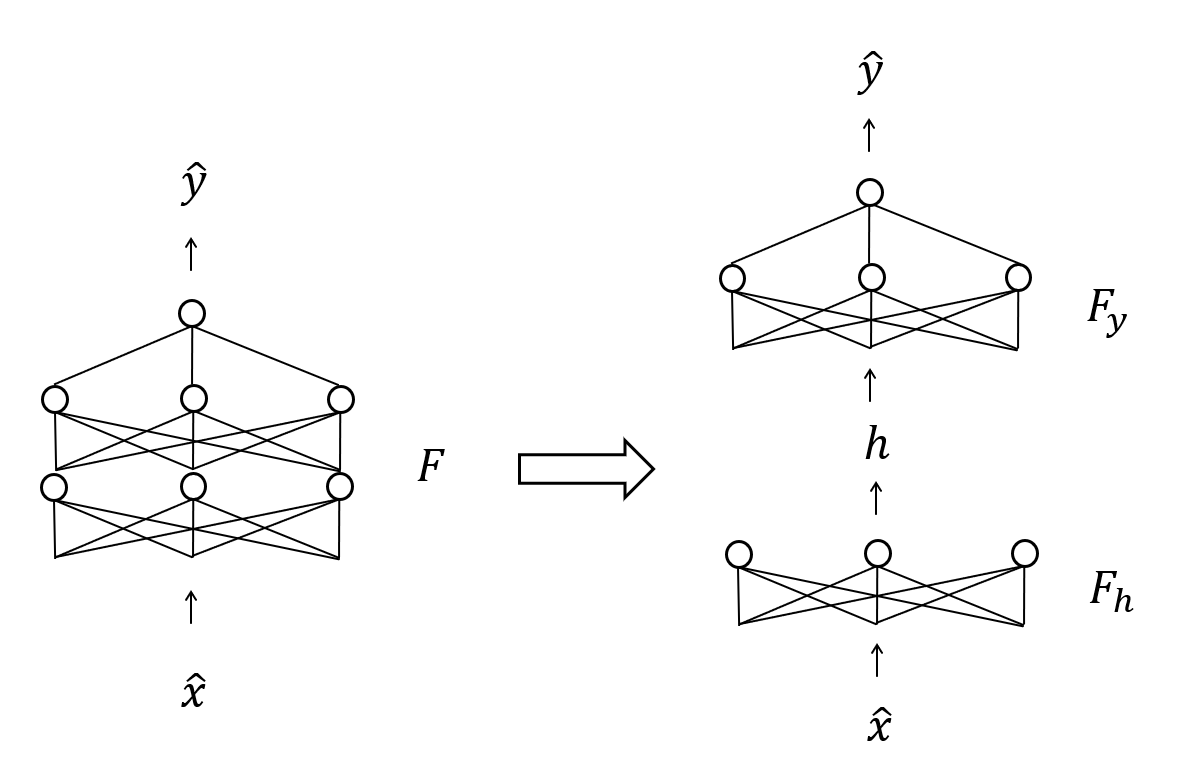
\includegraphics[width=0.35\textwidth]{split.png}
    \caption{Illustration of the split of neural network $\mathcal{F}$}
    \label{fig:split}
\end{figure}


$\left\{ \mathbf{h}^{(i)} \right\}_{i=1}^N$ can be split into positive and negative examples. For example, say `Thai' as the L1 language is a concept. $\boldsymbol{h_{pos}^{(i)}}$ originates from Thai candidates, and $\boldsymbol{h_{neg}^{(i)}}$ originates from non Thai candidates.

A simple linear classifier is trained among $\boldsymbol{h}$, with a linear decision boundary separating positive and negative outputs. The classifier is trained with hinge-loss minimization with L2-norm penalty, which penalizes extreme weights. The loss function is in equation \ref{eq:hinge-loss}:

\begin{equation} \label{eq:hinge-loss}
    \mathcal{L}(\boldsymbol{d^{(c)}}, b) = \sum_{i=1}^{N} w_{t^(i)} \mathrm{max} \{0, 1 - t^{(i)}(\boldsymbol{d}^{(c)T}\boldsymbol{h}^{(i)} + b)\} + \alpha \|\boldsymbol{d^{(c)}}\|_2^2
\end{equation}

where $t^{(i)} \in \{1, -1\}$ is the target label, where $t = 1$ for positive examples and $t = -1$ for negative examples, $w_{t^{(i)}}$ is the weighting for the i-th sample with target label $t^{(i)}$, and $\alpha$ is the regularization parameter that controls the strength of the L2-norm penalty.

The loss function maximizes the margin, as it encourages pushing as many data points away from the margin as possible. The L2-norm penalty is used to prevent overfitting from maximizing a particular weight, through adding a regularization term to the loss function. The linear decision boundary could be defined with the equation $\boldsymbol{d}^{(c)T}\boldsymbol{h} + b = 0$. The concept activation vector $\boldsymbol{d^{(c)}}$ of concept $c$ is the normal vector to the decision boundary. A 2-dimensional example is illustrated in Figure \ref{fig:linear}.

\begin{figure}[H]
    \centering
    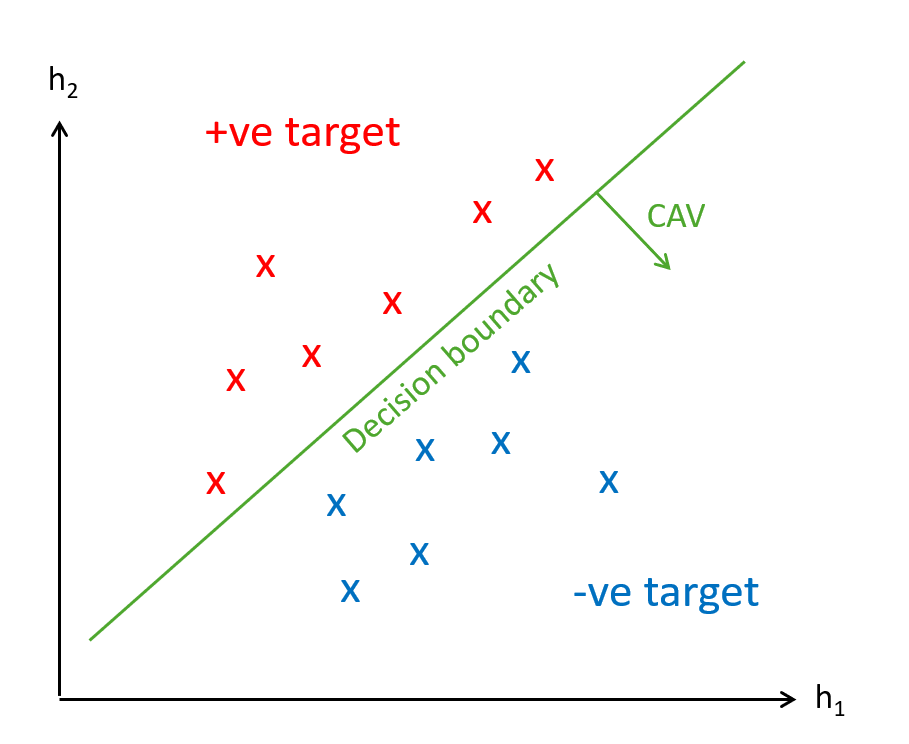
\includegraphics[width=0.35\textwidth]{linear.png}
    \caption{Illustration of CAV extraction. $h_1$ and $h_2$ represents  $\boldsymbol{h}$'s two dimensions}
    \label{fig:linear}
\end{figure}

The value of $w_{t^{(i)}}$ depends on the type of weighting used. In previous work, no weighting is used when extracting CAV, which essentially set $w_{t^{(i)}} = 1$ \cite{feature_bias}. Balanced weighting, on the other hand, set $w_{t^{(i)}} \propto \frac{1}{N_{i}}$, with $N_i$ being the number of samples with the same target label as $t^{(i)}$. Since balanced weighting assigns higher weights to underrepresented classes, it ensures that the classifier does not become biased towards the majority class. Since the use of weighting is found to generally improves the performance of machine learning methods \cite{balanced}, this paper would extract CAV with both methods, and compare the results.

\section{Perturbation of CAV}

Perturbation of the network is done by adding $\boldsymbol{\Delta h}$, which is along the CAV, to the activation layer's vector $\boldsymbol{h}$. The calculation of $\boldsymbol{\Delta h}$ is represented in equation \ref{eq:perturb}.

\begin{equation} \label{eq:perturb}
    \boldsymbol{\Delta h}^{(c)} = \left(\frac{1}{N}\sum_{i=1}^{N} \|\boldsymbol{h}^{(i)}\|_{2}) \right) \frac{ \boldsymbol{d}^{(c)}}{\| \boldsymbol{d}^{(c)}\|_2}
\end{equation}

Perturbation along the CAV could be represented as a linear combination of the CAV and the original vector $\boldsymbol{h}$. Figure \ref{fig:perturbation} illustrates the perturbation of a 2-dimensional activation, and the perturbation could be added to the system in the form of equation \ref{eq:add_perturbation}.

\begin{equation} \label{eq:add_perturbation}
    \mathcal{F}_{y}(\boldsymbol{h}^{(i)}; \boldsymbol{\theta}) \qquad \rightarrow \qquad \mathcal{F}_{y}(\boldsymbol{h}^{(i)} + \alpha \boldsymbol{\Delta h}^{(c)}; \boldsymbol{\theta})
\end{equation}

where $\alpha$ is the perturbation factor, a hyperparameter that controls the strength of the perturbation.

\begin{figure}[H]
    \centering
    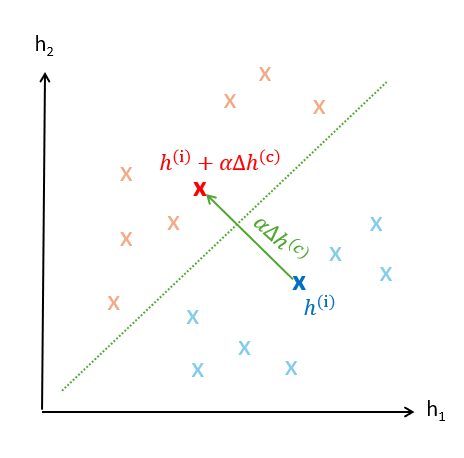
\includegraphics[width=0.35\textwidth]{perturbation.png}
    \caption{Illustration of CAV perturbation}
    \label{fig:perturbation}
\end{figure}

As illustrated in Figure \ref{fig:perturbation}, $\boldsymbol{\Delta h}^{(c)}$ moves the activation closer to the positive examples, which makes $\boldsymbol{h}$ more `positive' in the sense of the concept. For concepts that are not related to the grading process, the perturbation would not change the prediction of an unbiased model. However, for concepts that are related to the grading process, the perturbation should change the prediction. For example, perturbing the CAV of `male' makes a sample more `male' in the sense of the concept. As gender is not an assessing criteria, the predicted score should not change. In contrast, perturbing the CAV of `high speaking grade' makes the sample possess qualities of a stronger candidate, which should improve the prediction.

\section{Gradient-based Method} \label{sec:gradient}

As illustrated in Figure \ref{fig:relevant}, when $\boldsymbol{\Delta h}^{(c)}$ changes the score prediction, the direction is said to be align with $\frac{\partial \mathcal{F}_y}{\partial \boldsymbol{h}}$, the gradient of the network with respect to the activation of a particular layer. \nomenclature[A]{$\frac{\partial \mathcal{F}_y}{\partial \boldsymbol{h}}$}{Gradient of the Network With Respect to the Activation of a Particular Layer} Otherwise, as shown in Figure \ref{fig:irrelevant}, the direction is said to be orthogonal to $\frac{\partial \mathcal{F}_y}{\partial \boldsymbol{h}}$. The more aligned $\boldsymbol{\Delta h}^{(c)}$ is with the gradient, the greater the change in the predicted score after perturbation. For DNN, $\frac{\partial \mathcal{F}_y}{\partial \boldsymbol{h}} = \frac{\partial \mathbf{\hat{y}}}{\partial \boldsymbol{h}}$. For DDN, as the focus is on the predicted score and not the variance, $\frac{\partial \mathcal{F}_y}{\partial \boldsymbol{h}} = \frac{\partial \mathbf{\mu}}{\partial \boldsymbol{h}}$. As $\boldsymbol{\Delta h}^{(c)}$ is a scalar multiple of the CAV $\boldsymbol{d}^{(c)}$, the alignment could simply be compared between $\boldsymbol{d}^{(c)}$ and $\frac{\partial \mathcal{F}_y}{\partial \boldsymbol{h}}$.

\begin{figure}[H]
    \centering
    \begin{subfigure}{0.45\textwidth}
        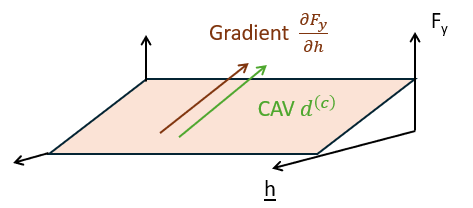
\includegraphics[width=\textwidth]{relevant.png}
        \caption{Gradient direction with CAV of relevant concept}
        \label{fig:relevant}
    \end{subfigure}
    \hfill
    \begin{subfigure}{0.45\textwidth}
        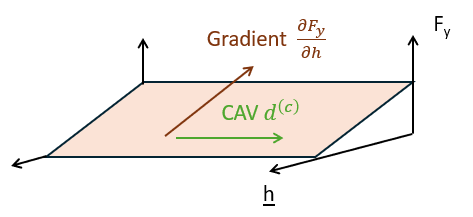
\includegraphics[width=\textwidth]{irrelevant.png}
        \caption{Gradient direction with CAV of irrelevant concept}
        \label{fig:irrelevant}
    \end{subfigure}
\end{figure}

Cosine distance ($\cos(\boldsymbol{a}, \boldsymbol{b})$) is used to compute the alignment. The cosine distance is defined in equation \ref{eq:cosine_distance}:

\begin{equation} \label{eq:cosine_distance}
    \cos(\boldsymbol{a}, \boldsymbol{b}) = 1 - \frac{\boldsymbol{a}^T \boldsymbol{b}}{\|\boldsymbol{a}\|_2 \|\boldsymbol{b}\|_2}
\end{equation}

which is 1 when $\boldsymbol{a}$ and $\boldsymbol{b}$ are orthogonal, and deviates from 1 when they are aligned. For an unbiased system's measurement with CAV of irrelevant concepts, the cosine distance should be 1.

To understand individual candidate's bias, the individual gradient cosine distance $\mathcal{B}^{(ci)}_{gr}$, formed between the CAV $\boldsymbol{d}^{(c)}$ and the individual candidate's gradient $\frac{\partial \mathcal{F}_y}{\partial \boldsymbol{h}}$, could be computed. The individual cosine distance is defined in equation \ref{eq:grad_individual}.  \nomenclature[A]{$\mathcal{B}^{(ci)}_{gr}$}{Individual Gradient Cosine Distance}

\begin{equation} \label{eq:grad_individual}
    \mathcal{B}^{(ci)}_{gr} = \cos\left(\boldsymbol{d}^{(c)}, \frac{\partial \mathcal{F}_y(\boldsymbol{h})}{\partial \boldsymbol{h}}\vert_{\boldsymbol{h^{(i)}}} \right)
\end{equation}

To understand the overall system's bias, the cosine distance between $\boldsymbol{d}^{(c)}$ and $\frac{\partial \mathcal{F}_y}{\partial \boldsymbol{h}}$ could be measured in two ways. The first way, overall gradient distance $\mathcal{B}^{(c)}_{\nabla}$, \nomenclature[A]{$\mathcal{B}^{(c)}_{\nabla}$}{Overall Gradient Cosine Distance} is between the CAV $\boldsymbol{d}^{(c)}$ and the average gradients $\frac{\partial \mathcal{F}_y}{\partial \boldsymbol{h}}$ from all data in equation \ref{eq:grad_del}, which is a faster method to compute for the gradient distance. Another way, the average gradient cosine distance $\mathcal{B}^{(c)}_{gr}$, is averaging the individual cosine distance formed, as shown in equation \ref{eq:grad_gr}. This method allows isolation of gradient distance for each sample, providing more insights for analysis.

\begin{equation} \label{eq:grad_del}
    \mathcal{B}^{(c)}_{\nabla} = \cos\left(\boldsymbol{d}^{(c)}, \frac{1}{N} \sum_{i=1}^{N} \frac{\partial \mathcal{F}_y(\boldsymbol{h})}{\partial \boldsymbol{h}}\vert_{\boldsymbol{h^{(i)}}} \right)
\end{equation}

\begin{equation} \label{eq:grad_gr}
    \mathcal{B}^{(c)}_{gr} = \frac{1}{N} \sum_{i=1}^{N} \mathcal{B}^{(ci)}_{gr} = \frac{1}{N} \sum_{i=1}^{N}\cos\left(\boldsymbol{d}^{(c)}, \frac{\partial \mathcal{F}_y(\boldsymbol{h})}{\partial \boldsymbol{h}}\vert_{\boldsymbol{h^{(i)}}} \right)
\end{equation}

When $\mathcal{B} > 1$, the CAV $\boldsymbol{d}^{(c)}$ is along the same direction as the gradient, indicating that the concept biases the system to increase the predicted score. When $\mathcal{B} < 1$, the CAV $\boldsymbol{d}^{(c)}$ is along opposite direction to the gradient, indicating the concept biases the system to decrease the predicted score.

\section{Assumptions}
To allow the CAV method to accurately measure the bias, the components in the workflow (input data, model under investigation, linear classifier for CAV extraction) should satisfy the following assumptions:

The true score from human graders should be unbiased. CAV only has the ability to detect presence within a trained model, but it cannot isolate whether the cause is due to the data or the model itself. If the input data is biased, even if the model is not inherently biased, the trained model would still become biased. A way to verify the assumption is to check the average score of input data of different concepts (see Section \ref{sec:data_construction}). For concepts irrelevant to performance, the average score should be similar.

The model should be reasonably accurate. If the model is inaccurate, the activation $\boldsymbol{h}$ would unlikely be representing the concepts accurately. To verify the assumption, the model's accuracy could be checked with the testing set. The model should be able to predict the score with low error (see Section \ref{sec:grader_performance}).

The activations should be linearly separable. There could be a case in Figure \ref{fig:overlap} where the activations $\boldsymbol{h}$ are simply too overlapped, such that any classifier could not differentiate between the two classes. Even if the activations $\boldsymbol{h}$ are separable, it should be by a linear classifier, rather than a non-linear decision boundary in Figure \ref{fig:non_linear}, as the CAV is the orthogonal vector to the decision boundary. Otherwise, a linear decision boundary with low accuracy would be trained, shown as the dotted line in the figure. The more accurate the linear classifier, the more representative the CAV is for the related concept. This could be verified by checking the accuracy of the linear classifier in differentiating positive and negative examples (see Section \ref{sec:cav_accuracy}).


\begin{figure}[H]
    \centering
    \begin{subfigure}{0.48\textwidth}
        \centering
        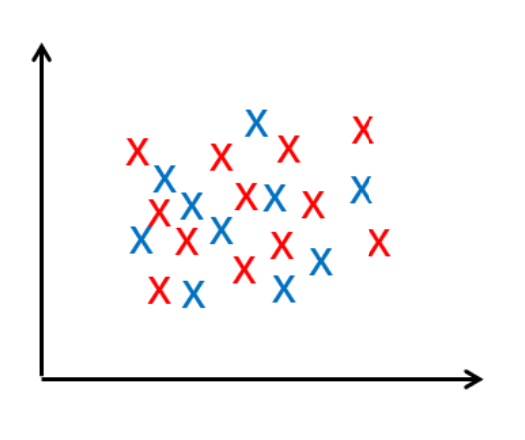
\includegraphics[width=0.5\textwidth]{overlap.png}
        \caption{Activations that are closely overlapped}
        \label{fig:overlap}
    \end{subfigure}
    \hfill
    \begin{subfigure}{0.48\textwidth}
        \centering
        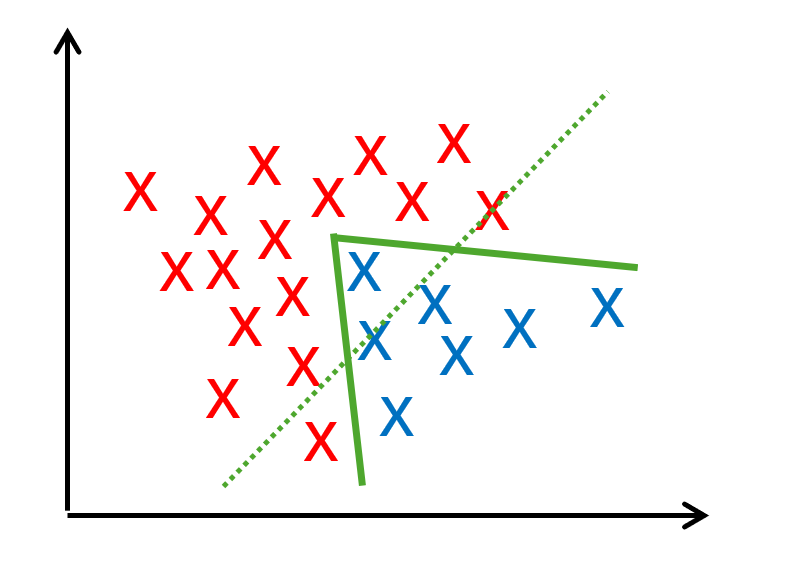
\includegraphics[width=0.5\textwidth]{non_linear.png}
        \caption{Activations with non-linear decision boundary}
        \label{fig:non_linear}
    \end{subfigure}
\end{figure}

\section{Summary}
This chapter discussed the CAV method, highlighting how it could be used to detect bias in a model. The mathematical details on how to extract CAV from the model, how to perturb the activation along the CAV, and how to measure bias through alignment of CAV with the gradient were discussed. The assumptions of the CAV method were also discussed, including that the input data is unbiased and that the activation is linearly separable. This outlines the foundation to measure the models' bias in the upcoming chapters.
\chapter{Data and Experimental Setup} \label{chap:setup}

\section{Training, Calibration, and Testing}

\subsection{Data Construction} \label{sec:data_construction}
The dataset comprises responses from candidates taking the Linguaskill exams for second language (L2) \nomenclature[Z]{L2}{Second Language} learners of English. These exams are divided into five sections, each scored on a scale from 0 to 6. This study focuses on Part 1, where candidates answer eight questions about themselves \cite{linguaskills}. Candidates are provided 10 seconds to respond to the first four, and 20 seconds for the last four. The first two questions are not graded. Overall, the candidates' performance across all sections is mapped to CEFR levels ranging from A1 to C2 \cite{CEFR}.

For text-based model, the dataset contains the response transcripts extracted from the audio files. For feature-based model, the dataset contains the 356-dimensional features extracted from the audio files. For audio-based model, the dataset contains the audio represented in vector format. Each item in the dataset has an associated candidate number to identify the candidate, and the corresponding score from the human graders.

The dataset is divided into three sections: training, calibration, and testing. The training set is used to train the model, the calibration set is used to tune linear calibration after the score prediction from the neural network (Chapter \ref{chap:graders}), and the testing set is used to evaluate the model's performance. Table \ref{tab:data_size} shows the number of candidates in each section of the dataset.

\begin{table}[H]
    \centering
    \begin{tabular}{|c|c|c|}
        \hline
        \textbf{Training} & \textbf{Testing} & \textbf{Calibration} \\ \hline
        31471             & 1048             & 1033                 \\ \hline
    \end{tabular}
    \caption{Number of candidates in each section of the dataset}
    \label{tab:data_size}
\end{table}

The metadata about the candidates are also provided, including their age, gender, and first language. Based on the metadata, four distinct groups of concepts were identified: grades, categorized as $\leq$ A2 ($\leq$ 2.0), $\geq$ B2 ($\geq$ 4.0), and $\geq$ C1 ($\geq$ 5.0); first language, with Thai and Spanish chosen for the experiment; young candidates, defined as those aged $\leq$ 30; and male gender. As grade concepts are definitely correlated to the scores output, it is expected that `bias' could be detected with the CAV method. Hence, the grade concepts exist to help verify the CAV's bias-detecting ability. On the other hand, the model is most likely unbiased towards the non-grade concepts, hence it could be used to observe the CAV's performance in the absence of bias. The non-grade concepts are also chosen to be diverse, such that bias measurement could be compared across different concepts.

To verify that the dataset is unbiased, the average scores across the training, calibration, and testing sets were calculated for each group of concepts, shown in Table \ref{tab:avg_scores}. The scores for candidates having that concepts (positive target) and not having that concepts (negative target) are both included. Values out of the range of 3 to 4 are highlighted in red. Except for an outlying Thai -ve target score of 2.90 from the calibration set, the average scores for all non-grade concepts are within the range of 3 to 4, indicating a balanced distribution of scores across the dataset. The average scores for positive targets from grade concepts are out of the range, with $\leq$ A2, $\geq$ B2, and $\geq$ C1 having average scores of 2.48, 4.29, and 5.15 respectively, which is expected based on the cutoff of the CEFR levels. It could be concluded that the dataset is not biased towards any specific group of candidates under consideration.

\begin{table}[H]
    \centering
    \begin{tabular}{|lc|c|c|c|c|c|c|c|}
        \hline
        \multicolumn{2}{|l|}{\textbf{}}                            & \textbf{\textless{}A2} & \textbf{\textgreater{}B2} & \textbf{\textgreater{}C1} & \textbf{Thai}         & \textbf{Spanish}      & \textbf{Male} & \textbf{Young}        \\ \hline
        \multicolumn{1}{|l|}{\multirow{2}{*}{\textbf{Training}}}   & \textbf{+ve target}    & \textcolor{red}{2.48}     & \textcolor{red}{4.29}     & \textcolor{red}{5.15} & 2.99                  & 3.61          & 3.41           & 3.56 \\ \cline{2-9}
        \multicolumn{1}{|l|}{}                                     & \textbf{-ve target}    & 3.67                      & 3.19                      & 3.40                  & 3.55                  & 3.25          & 3.41           & 3.21 \\ \hline
        \multicolumn{1}{|l|}{\multirow{2}{*}{\textbf{Testing}}}    & \textbf{+ve target}    & \textcolor{red}{2.25}     & \textcolor{red}{4.54}     & \textcolor{red}{5.13} & 3.02                  & 3.44          & 3.57           & 3.73 \\ \cline{2-9}
        \multicolumn{1}{|l|}{}                                     & \textbf{-ve target}    & \textcolor{red}{4.12}     & 2.88                      & 3.37                  & 3.64                  & 3.59          & 3.53           & 3.15 \\ \hline
        \multicolumn{1}{|l|}{\multirow{2}{*}{\textbf{Calbration}}} & \textbf{+ve target}    & \textcolor{red}{2.36}     & \textcolor{red}{4.46}     & \textcolor{red}{5.14} & \textcolor{red}{2.90} & 3.44          & 3.51           & 3.58 \\ \cline{2-9}
        \multicolumn{1}{|l|}{}                                     & \textbf{-ve target}    & 3.96                      & 2.97                      & 3.39                  & 3.58                  & 3.50          & 3.25           & 3.33 \\ \hline
    \end{tabular}
    \caption{Average scores for each type of concepts}
    \label{tab:avg_scores}
\end{table}

\subsection{Process of Training, Calibration, and Testing}

\begin{figure}[H]
    \centering
    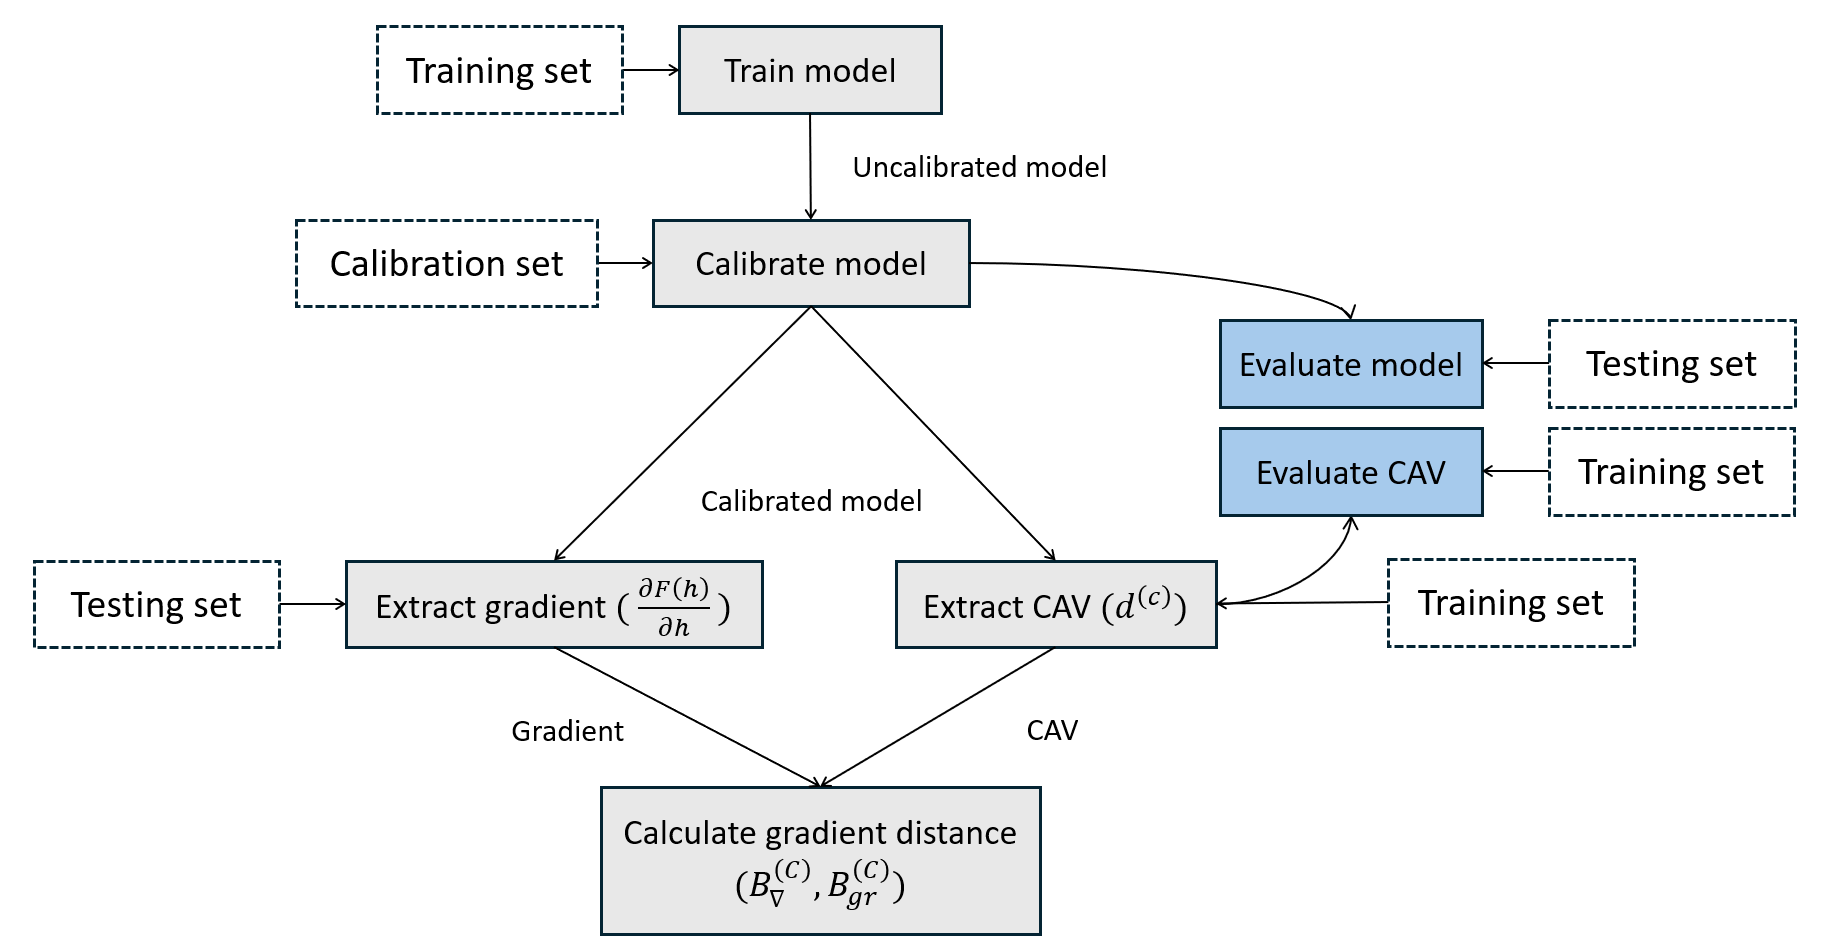
\includegraphics[width=0.95\textwidth]{flow.png}
    \caption{Flow of the process to obtain the bias measurement with gradient distance}
    \label{fig:flow}
\end{figure}

Figure \ref{fig:flow} illustrates the process requires to obtain the bias measurement with gradient distance. The grey boxes represents the main steps of the process. The first step is to train the parameters in the model $\mathcal{F}$, through minimizing the MSE loss function (Equation \ref{eq:mse}) for DNN, and NLL loss function (Equation \ref{eq:nll}) for DDN. Afterwards, the neural network parameters are frozen, and the slope $m$ and intercept $c$ of the subsequent linear regression model (Equation \ref{eq:calibration}) are trained, also through minimizing the MSE loss function. The trained model is then passed with input data, with the gradients $\frac{\partial \mathcal{F}_y}{\partial \boldsymbol{h}}$ and the activation $\boldsymbol{h}$ in the layers tracked for each input. In this experiment, only the gradient and activation from the first layer are investigated. $\boldsymbol{h}$ from all inputs are collected to train a simple linear classifier to differentiate the concept of interest. Through minimizing the hinge-loss function (Equation \ref{eq:hinge-loss}), the CAV $\boldsymbol{d^{(c)}}$ is obtained through the decision boundary. Finally, the gradients $\frac{\partial \mathcal{F}}{\partial \boldsymbol{h}}$ and CAV $\boldsymbol{d^{(c)}}$ are used to calculate the gradient distance $\mathcal{B}^{(c)}_{\nabla}$ (Equation \ref{eq:grad_del}) and $\mathcal{B}^{(c)}_{\nabla}$ (Equation \ref{eq:grad_gr}).

The blue boxes represent the performance evaluation steps that could be done throughout the flow, including the model and the CAV accuracy, using the assessment criteria in section \ref{sec:performance_criteria}.

Finally, the dotted white boxes represent the data used in each step. It refers to where is the source of the intermediate vector $\mathbf{\hat{x}}$ passed into the system $\mathcal{F}$. To highlight, while the testing set is used for model evaluation, the training set is used for CAV evaluation. This choice is made as the CAV evaluation is to measure how accurately the CAV represents the concept during the training process itself.

\section{Hyper-parameters}
\subsection{Model Training}
The model architecture hyper-parameter used for training has been outlined in Chapter \ref{chap:graders}, which includes the layer number, node number, activation function, dropout rate and the model type (DNN vs DDN) hence the minimization function (MSE vs NLL).

All the trainings are done on CUDA with the NVIDIA Tesla V100S-PCIe GPU with 32GB memory, using the PyTorch library. The following explains the training hyper-parameters for each model:

The text-based model is trained for 2 epochs using an Adam optimizer with decoupled weight decay (AdamW) \nomenclature[Z]{AdamW}{Adam Optimizer with Decoupled Weight Decay}. The first and second epochs have a learning rate of $1 \times 10^{-5}$ and $1 \times 10^{-6}$ respectively. The model is trained with a batch size of 8, and the seed number is set to 5. Each seed's training process takes approximately 2 hours.

The feature-based model is trained for 200 epochs using an Adam optimizer with a learning rate of $1 \times 10^{-5}$. The model is trained with a batch size of 20, and the seed number is also set to 5. Each seed's training process also takes approximately 2 hours.

The audio-based model is trained for 4 epochs using an AdamW optimizer, which has a learning rate of $1 \times 10^{-6}$. The model is trained with a batch size of 32, and the seed number is set to 2, less than that of text and feature-based model. It is because the training process for each seed takes approximately 36 hours, hence it is computationally more feasible to compare with less seeds.


Table \ref{tab:training_hyper_param} summarizes the training hyper-parameters for each model.

\begin{table}[H]
    \centering
    \begin{tabular}{|l|c|c|c|}
        \hline
                                  & \textbf{Text-Based}                             & \textbf{Feature-Based} & \textbf{Audio-Based} \\
        \hline
        \textbf{Optimizer}        & AdamW                                           & Adam                   & AdamW                \\ \hline
        \textbf{Learning Rate}    & $1 \times 10^{-5} \rightarrow 1 \times 10^{-6}$ & $1 \times 10^{-5}$     & $1 \times 10^{-6}$   \\ \hline
        \textbf{Epochs}           & 2                                               & 200                    & 4                    \\ \hline
        \textbf{Batch Size}       & 8                                               & 20                     & 32                   \\ \hline
        \textbf{Seed number}      & 5                                               & 5                      & 2                    \\ \hline
        \textbf{Duration (hours)} & 2                                               & 2                      & 36                   \\ \hline
    \end{tabular}
    \caption{Training hyper-parameters for different model types}
    \label{tab:training_hyper_param}
\end{table}

\subsection{CAV Linear Classifier Training}
The CAV linear classifier follows the one implemented in \cite{feature_bias}. The regularization parameter $\alpha$ in equation \ref{eq:hinge-loss}, which controls the strength of L2-norm penalty, used a value of 0.001. Stochastic Gradient Descent is used as the optimizer, with the learning rate scheduled optimally using implementation from \verb|Scikit-learn| \cite{scikit-learn}. The training step is limited with 2000 iterations, and it steps when the MSE change is within $1 \times 10^{-4}$. Polyak–Ruppert averaging is used, which means the last 16 sets of CAV weights and bias are averaged as the output. The CAV is extractable within minutes.

\section{Model Biasing}
To understand how effective the bias measurement with CAV is, a biased model is trained through feeding in training data deliberately biased towards a specific concept. The biased model would also follow the same flow as the original model to calculate the gradient distance $\mathcal{B}^{(c)}_{\nabla}$ and $\mathcal{B}^{(c)}_{gr}$. The results are used to compare with the original model. If the original model is unbiased, and $\mathcal{B}^{(c)}_{\nabla}$ and $\mathcal{B}^{(c)}_{gr}$ could reflect the bias, it is expected that $\mathcal{B}^{(c)}_{\nabla}$ and $\mathcal{B}^{(c)}_{gr}$ of the concept being biased would still be close to 1 for the original model, but deviate from 1 for the biased one.

To bias the training data, all positive targets of the concept under consideration have their predicted score increased by 1. A maximum cap of 6 is applied for the increment, such that the scores would not exceed the maximum score of the exam.

\section{Factor Isolation}
Plotting the results of the bias measurement with individual candidates' gradient distance $\mathcal{B}^{(ci)}_{gr}$ against their predicted score, it is observed that feature-based models are more sensitive to bias measurement. To understand what factors are affecting $\mathcal{B}^{(ci)}_{gr}$'s pattern, particularly its sensitivity to bias measurement, the models are trained with different hyper-parameters, and their bias measurements are compared with the original models to isolate the factors. Text and feature-based models are chosen for comparison, as both text and audio-based models are based on the attention mechanism, while feature-based model is not. Between text and audio model, text-based model takes less time to train and evaluate, hence it is chosen for comparison.

The first factor considered is the network architecture. It is hypothesized that the layer number and node number would affect the pattern of $\mathcal{B}^{(ci)}_{gr}$. Hence, a new feature-based model is trained in Figure \ref{fig:bert_like}, but with the layer number, node number and dropout rate same as that of the text-based mode. The unchanged and changed components are in blue and red respectively. The input remains 356-dimensional for the feature vector, and the output remains 2-dimensional for the Gaussian mean $\mu$ and standard deviation $\sigma$ prediction. The activation function is also kept as LReLU.

\begin{figure}[H]
    \centering
    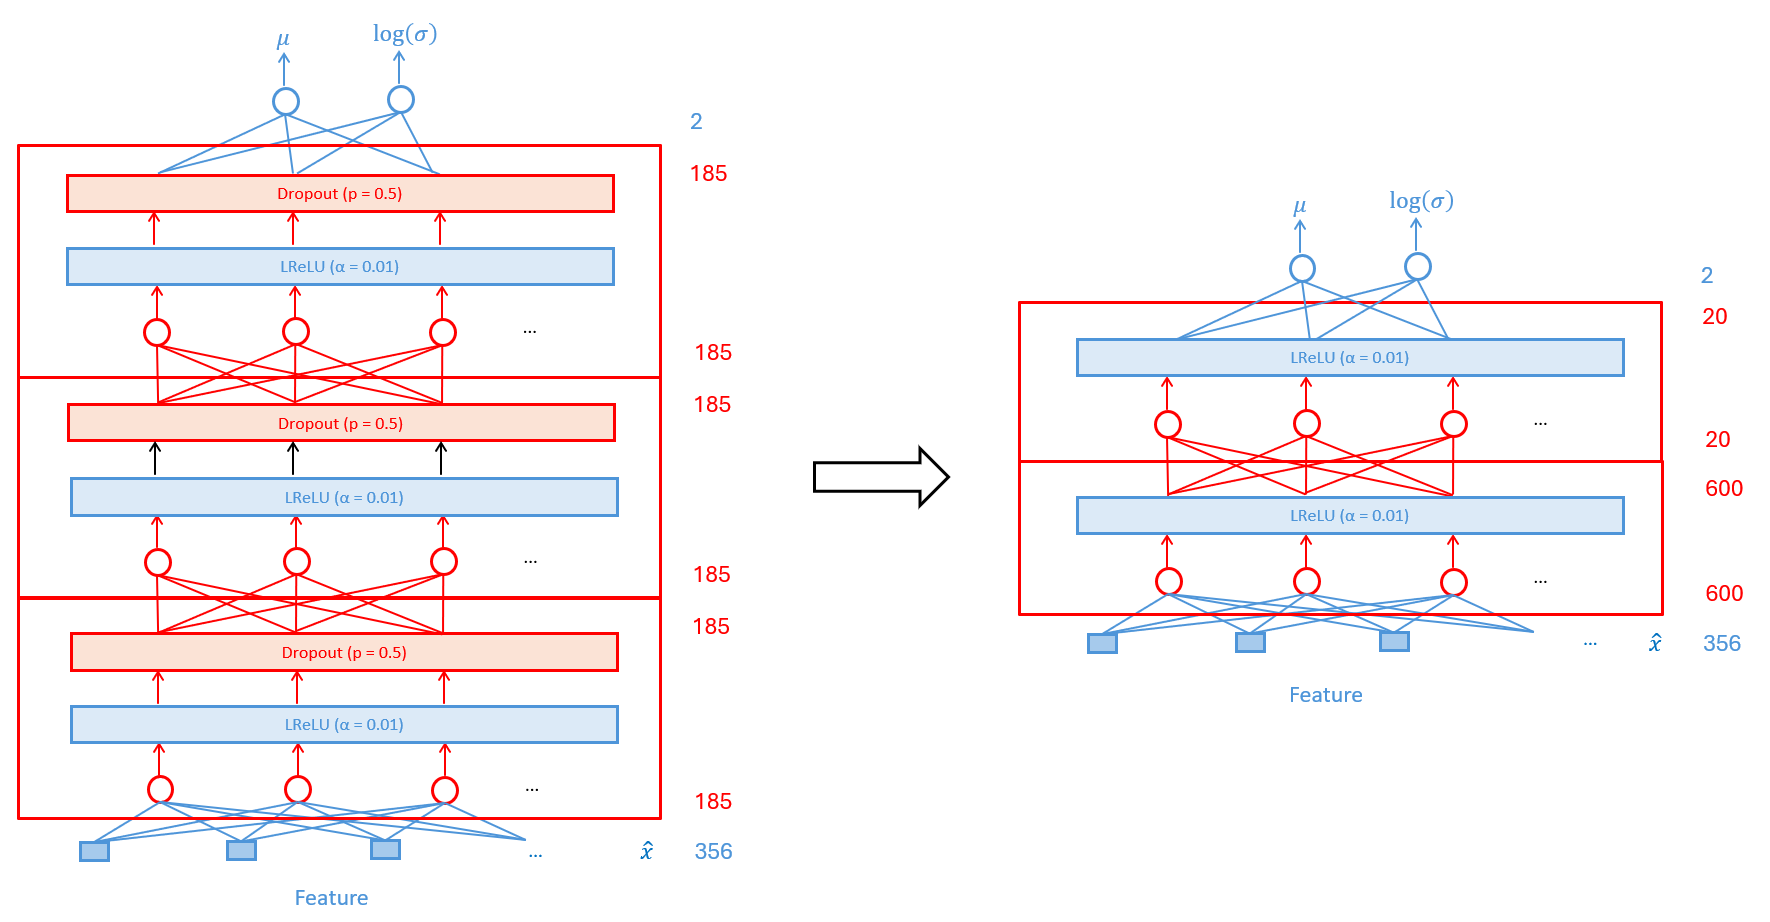
\includegraphics[width=0.85\textwidth]{bert_like.png}
    \caption{Change of feature-based model architecture similar to text-based model, with original (left) and new (right) architecture}
    \label{fig:bert_like}
\end{figure}

The second factor considered is the model type. It is hypothesized that the use of DNN would affect the pattern of $\mathcal{B}^{(ci)}_{gr}$. Hence, a new feature-based model is trained in figure \ref{fig:dnn_like}, but with the model type changed from DDN to DNN, while keeping the model architecture same as that of the original feature-based model. The loss function is subsequently also changed from MSE to NLL.

\begin{figure}[H]
    \centering
    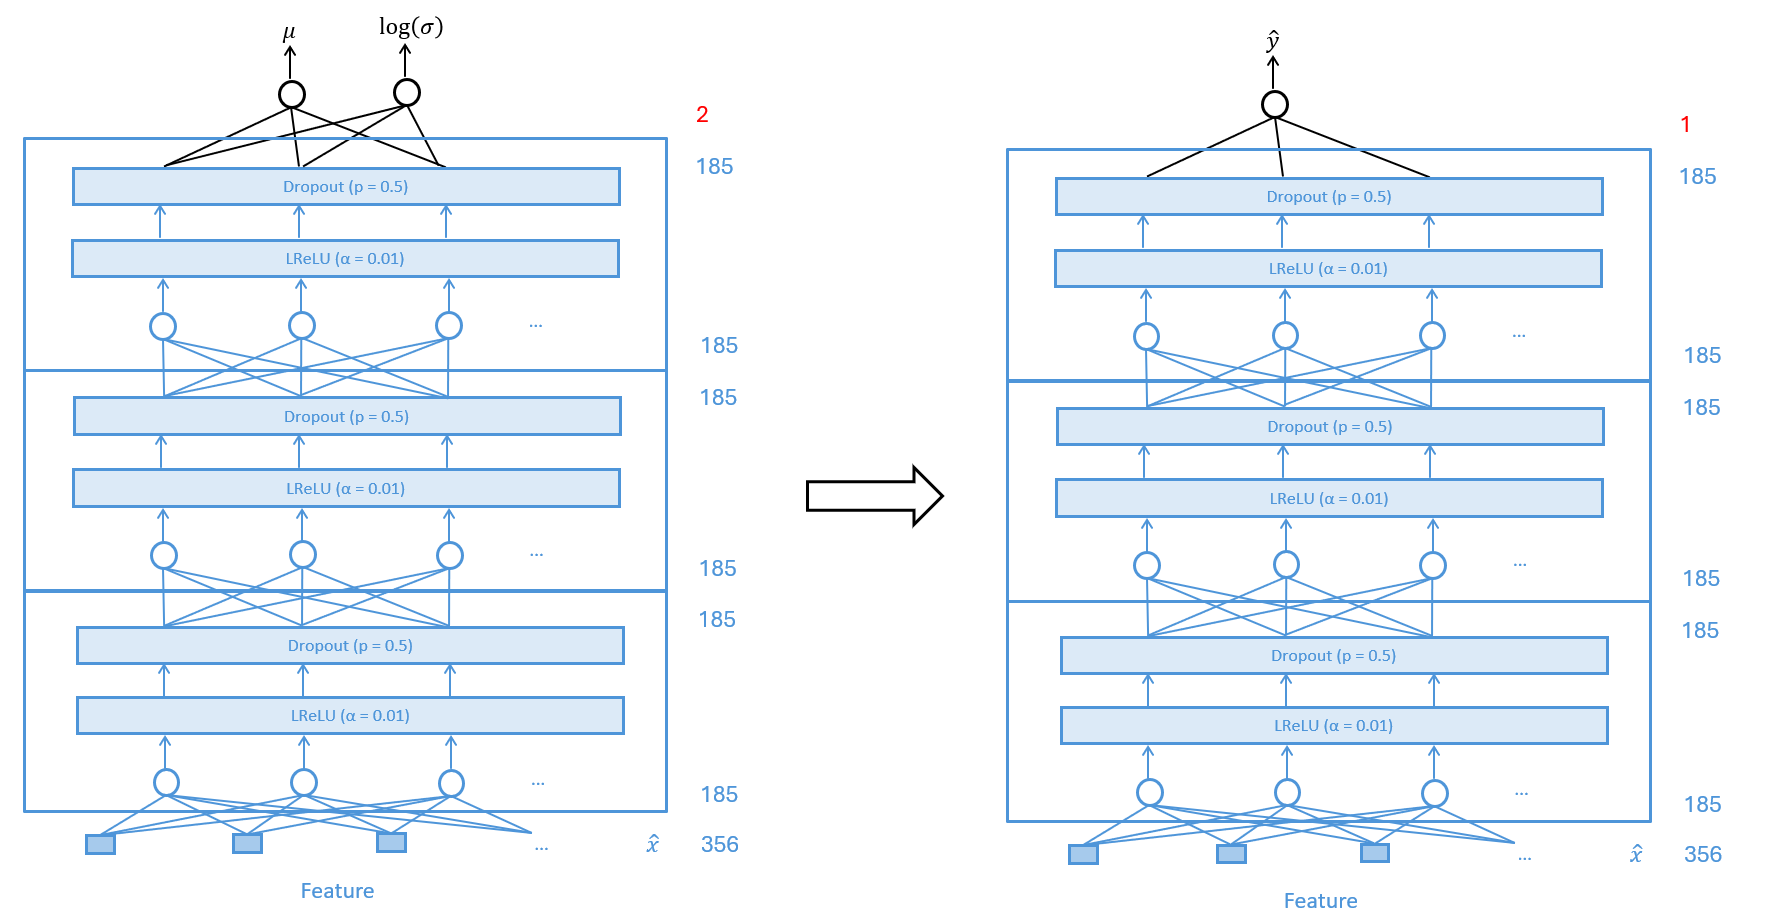
\includegraphics[width=0.85\textwidth]{dnn_like.png}
    \caption{Change of feature-based model from DDN (left) to DNN (right)}
    \label{fig:dnn_like}
\end{figure}

The third factor is the activation function. It is hypothesized that the use of LReLU would affect the pattern of $\mathcal{B}^{(ci)}_{gr}$. Hence, a new feature-based model is trained in figure \ref{fig:relu}. The activation function changed from LReLU to ReLU, which is the activation function used in the text and audio-based model. The model architecture is kept the same as that of the original feature-based model, and the loss function is kept as NLL.

\begin{figure}[H]
    \centering
    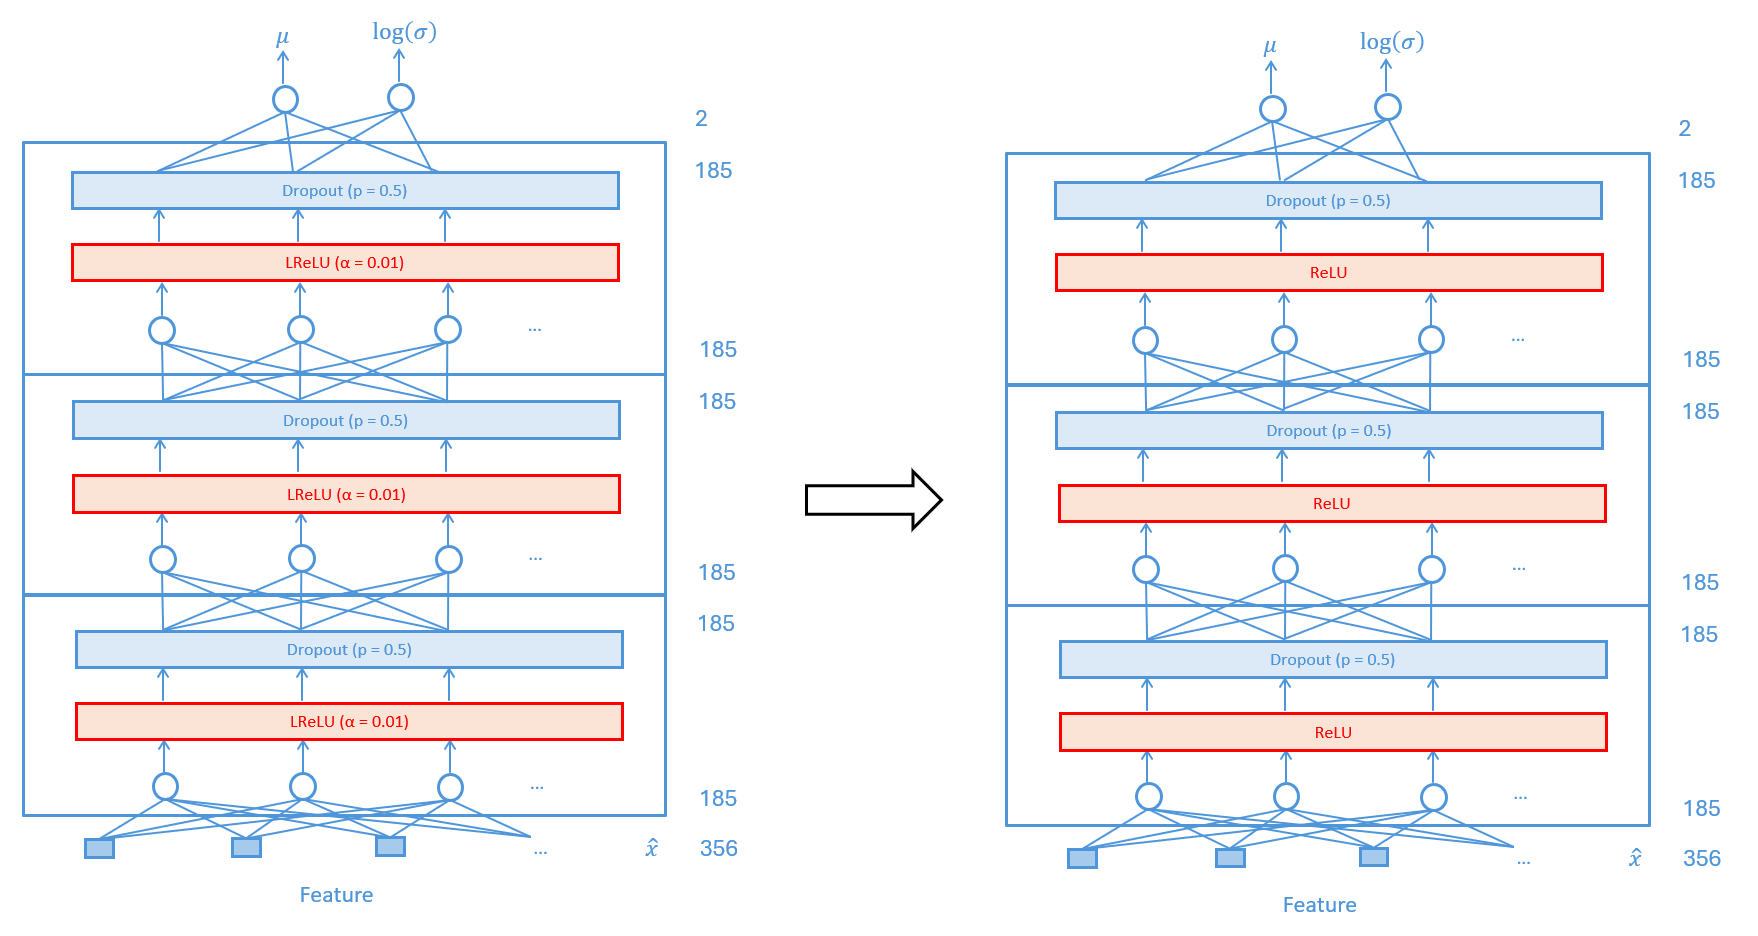
\includegraphics[width=0.85\textwidth]{relu.png}
    \caption{Change of feature-based model activation function from LReLU (left) to ReLU (right)}
    \label{fig:relu}
\end{figure}

In addition, a new text-based model is trained in figure \ref{fig:lrelu}, with the activation function changed from ReLU to LReLU, which is the activation function used in the feature-based model. The model architecture is kept the same as that of the original text-based model, and the loss function is kept as MSE.

\begin{figure}[H]
    \centering
    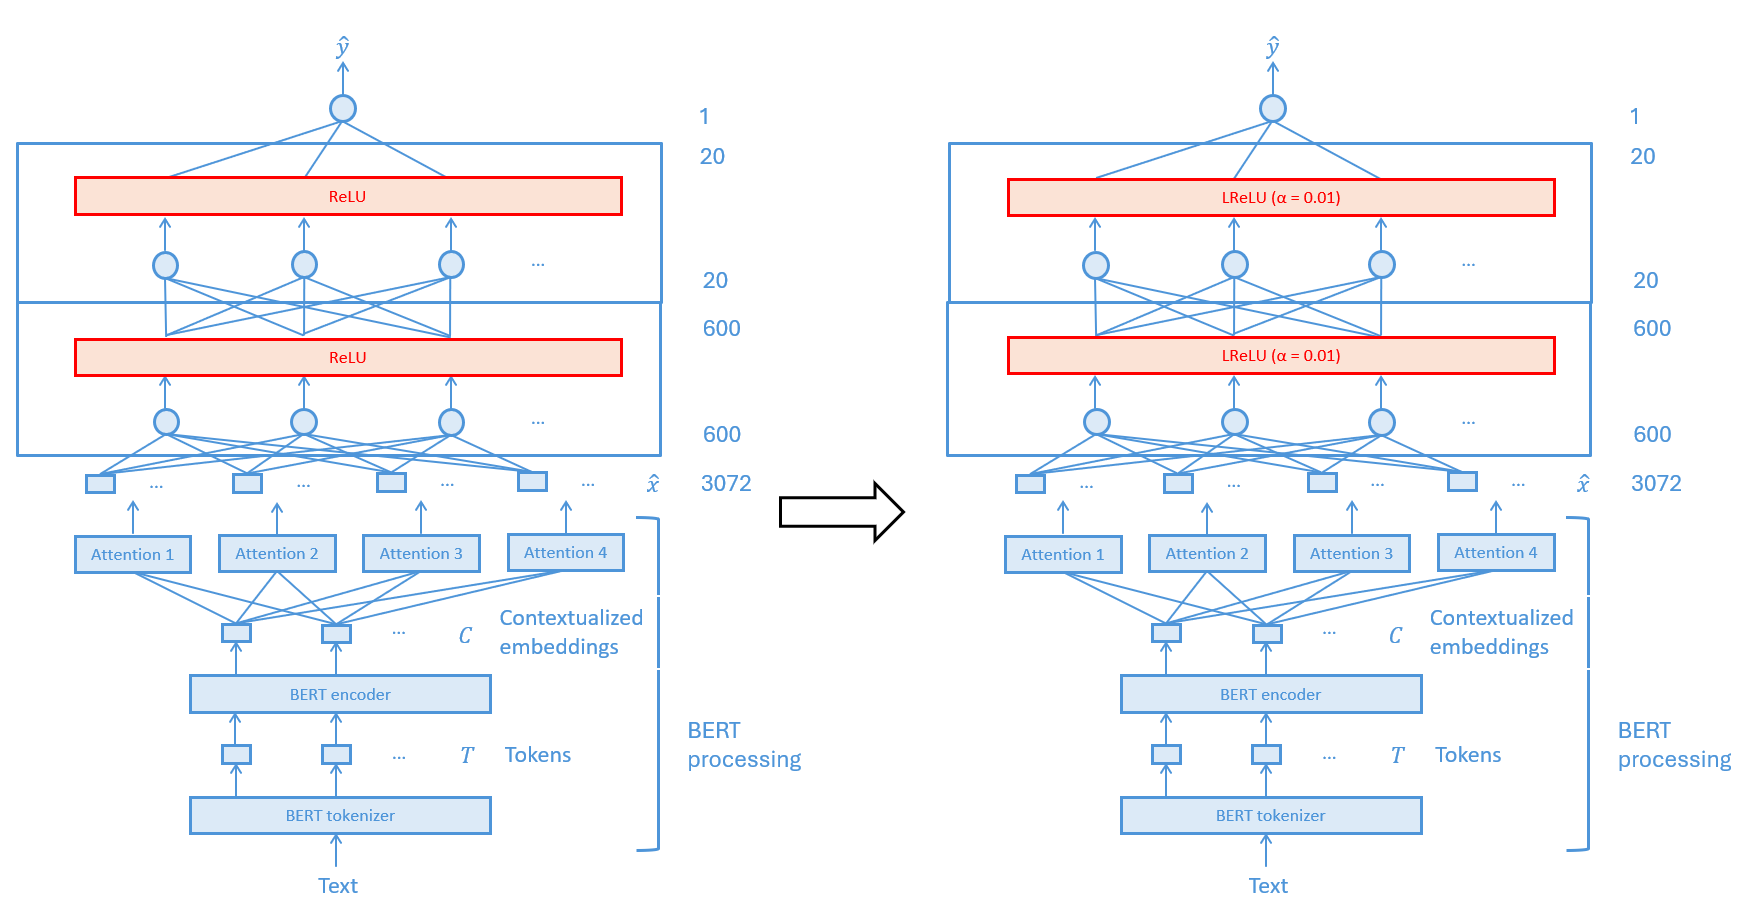
\includegraphics[width=0.85\textwidth]{lrelu.png}
    \caption{Change of text-based model activation function from ReLU (left) to LReLU (right)}
    \label{fig:lrelu}
\end{figure}

The fourth factor is the input. It is hypothesized that the nature of the input, whether it is vectors generated from attention mechanism, or feature vectors, would affect pattern of $\mathcal{B}^{(ci)}_{gr}$. Hence, the text-based model is modified to concatenate the attention embeddings $\mathbf{\hat{x}}$ with the feature vector, before passing it into the neural network. The network architecture remains the same as the text-based model, except the input dimension is now $3072 + 356 = 3428$-dimensional. The feature vector would only contribute to $10.4\%$ of the concatenated input vector, which is a rather small proportion only. The modification is shown in figure \ref{fig:deep_fusion}.

\begin{figure}[H]
    \centering
    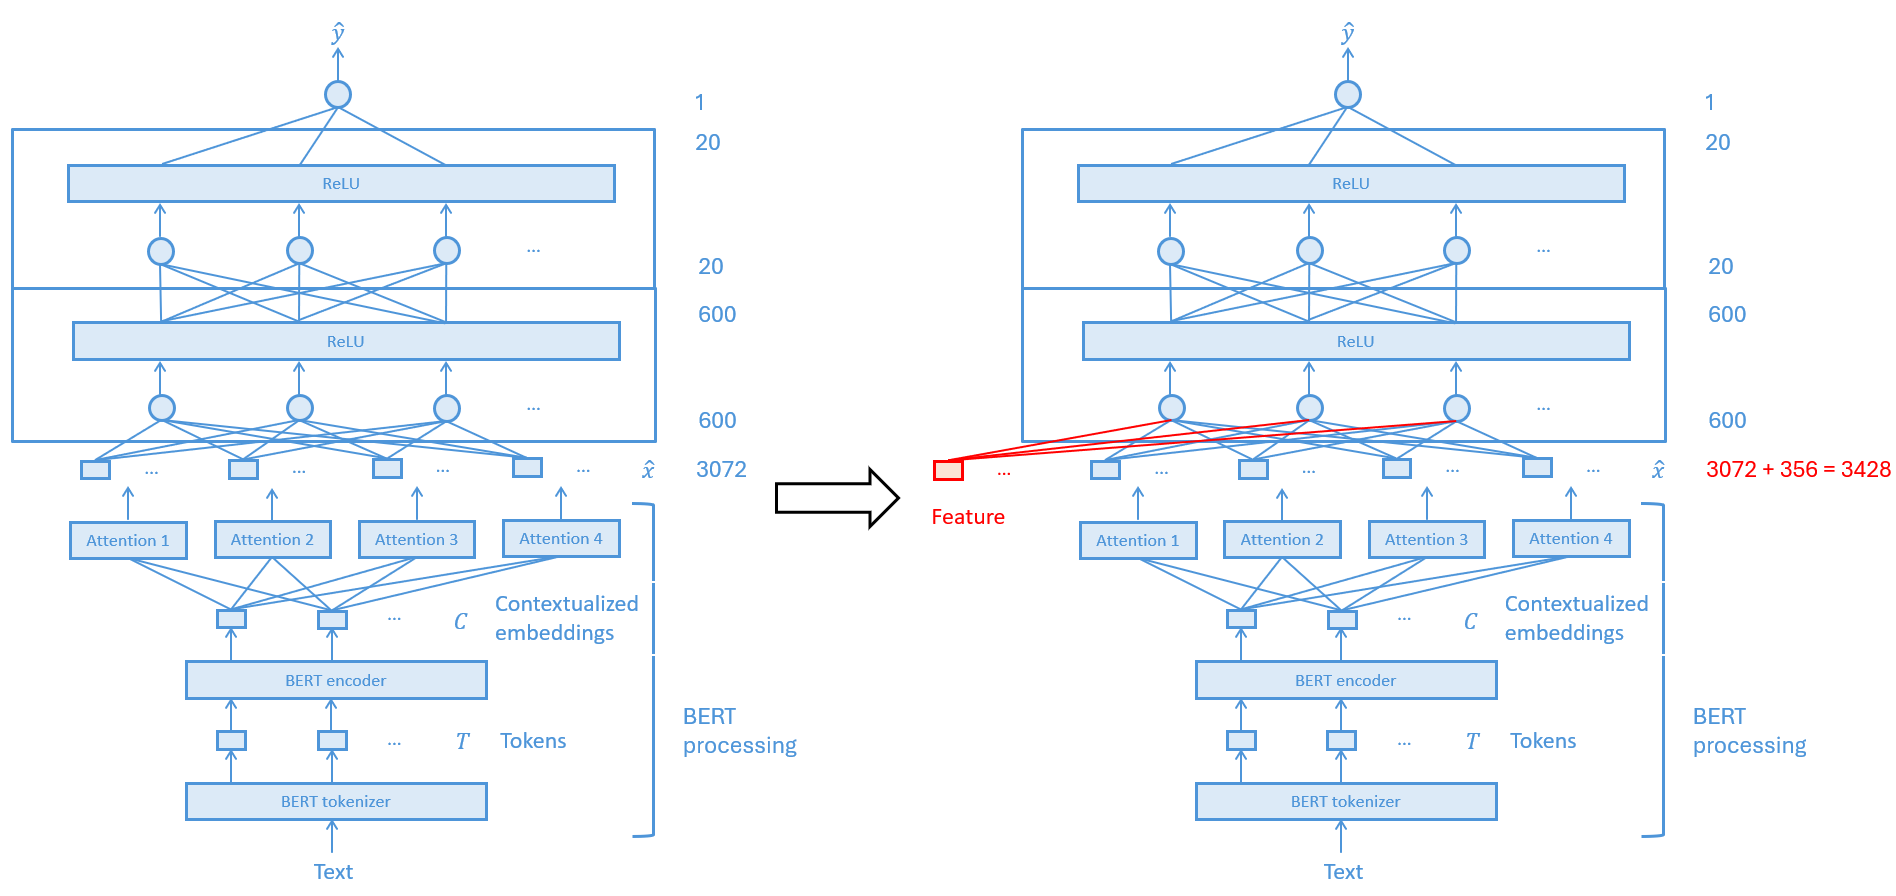
\includegraphics[width=0.85\textwidth]{deep_fusion.png}
    \caption{Deep fusion of feature vector and BERT attention embeddings, with original (left) and new (right) input method}
    \label{fig:deep_fusion}
\end{figure}

\section{Performance Criteria} \label{sec:performance_criteria}
\subsection{Model Performance}
The model's performance is evaluated with four criteria: the root mean square error (RMSE) and the Pearson correlation coefficient (PCC) \nomenclature[Z]{PCC}{Pearson Correlation Coefficient} between the predicted scores and the human graders' scores, the percentage of scores within 0.5 of the human graders' scores ($< 0.5$),  \nomenclature[Z]{$< 0.5$}{Percentage of Scores Within 0.5 of Human Graders'} and the percentage of scores within 1 of the human graders' scores ($< 1$) \nomenclature[Z]{$< 1$}{Percentage of Scores Within 1 of Human Graders'}.

The RMSE is calculated using Equation \ref{eq:rmse}, which is used to measure the accuracy of the model's predictions. A lower RMSE is desired as it indicates the model's prediction is closer to the actual scores given by the human graders.

\begin{equation} \label{eq:rmse}
    \text{RMSE} = \sqrt{\frac{1}{n} \sum_{i=1}^{n} (y_i - \hat{y}_i)^2}
\end{equation}

The PCC is calculated using Equation \ref{eq:pcc}, which measures the linear correlation between the predicted scores and the actual scores. A PCC value close to 1 indicates a strong positive correlation, a value close to -1 indicates a strong negative correlation, and a value close to 0 indicates no correlation. A PCC value closer to 1 is preferred, as it indicates that the model's predictions are closely aligned with the human graders' scores.

\begin{equation} \label{eq:pcc}
    \text{PCC} = \frac{\sum_{i=1}^{n} (y_i - \bar{y})(\hat{y}_i - \bar{\hat{y}})}{\sqrt{\sum_{i=1}^{n} (y_i - \bar{y})^2} \sqrt{\sum_{i=1}^{n} (\hat{y}_i - \bar{\hat{y}})^2}}
\end{equation}

where $y_i$ is the actual score given by the human graders, $\hat{y}_i$ is the predicted score by the model, $\bar{y}$ is the mean of the actual scores, and $\bar{\hat{y}}$ is the mean of the predicted scores.

For the percentage of scores within 0.5 and 1 of the human graders' scores, the percentage is calculated using Equation \ref{eq:within_05} and \ref{eq:within_1} respectively, where $n$ is the total number of candidates, and $y_i$ is the actual score given by the human graders, while $\hat{y}_i$ is the predicted score by the model. A higher percentage indicates that the model's predictions are closer to the human graders' scores, which is desired.

\begin{equation} \label{eq:within_05}
    \text{Percentage of Scores Within 0.5} = \frac{1}{n} \sum_{i=1}^{n} \mathbb{I}(|y_i - \hat{y}_i| < 0.5)
\end{equation}

\begin{equation} \label{eq:within_1}
    \text{Percentage of Scores Within 1} = \frac{1}{n} \sum_{i=1}^{n} \mathbb{I}(|y_i - \hat{y}_i| < 1)
\end{equation}
where $\mathbb{I}$ is the indicator function, which returns 1 if the condition is true, and 0 otherwise.

\subsection{CAV Performance}
The performance of CAV is evaluated with the accuracy of the linear classifier, which is trained to differentiate the concept of interest. The positive and negative target accuracy is calculated using Equation \ref{eq:pos_accuracy} and \ref{eq:neg_accuracy} respectively, where $TP$ is the number of true positives, $TN$ is the number of true negatives, $FP$ is the number of false positives, and $FN$ is the number of false negatives.

\begin{equation} \label{eq:pos_accuracy}
    \text{Positive Target Accuracy} = \frac{TP}{TP + FP}
\end{equation}

\begin{equation} \label{eq:neg_accuracy}
    \text{Negative Target Accuracy} = \frac{TN}{TN + FN}
\end{equation}

\subsection{Bias Measurement}
As mentioned in Section \ref{sec:gradient}, the bias measurement is calculated using the gradient distance $\mathcal{B}^{(c)}_{\nabla}$ and $\mathcal{B}^{(c)}_{gr}$. A plot of $\mathcal{B}^{(ci)}_{gr}$ against individual candidates' score could also be plotted. The bias measurement is expected to be close to 1 for an unbiased model, and deviate from 1 for a biased model. Hence, if the gap between the gradient distance between the biased and unbiased model is significant, it indicates that the bias measurement is effective in measuring the bias in the model.

\section{Summary}
This chapter outlines the data and experimental setup used in this study. The dataset is constructed from responses of candidates taking the Linguaskill exams, divided into training, calibration, and testing sets. The process of training, calibration, and testing is described, along with the hyper-parameters used for model training and CAV extraction. The chapter also discusses the model biasing process and factor isolation to understand the impact of different components on the bias measurement. Finally, the performance criteria for evaluating the model and CAV are defined.
\chapter{Experimental Results and Discussion} \label{chap:results}

\section{Grader Performance} \label{sec:grader_performance}
This section presents the performance of the grader models trained with the three different features: feature, text, and audio. Accurate models set foundation for the subsequent sections on bias detection and analysis.

The accuracy of the three models, both calibrated and uncalibrated, is presented in Table \ref{tab:model_accuracy}. The table shows the Root Mean Square Error (RMSE), Pearson Correlation Coefficient (PCC), and the percentage of predictions that are less than 0.5 ($< 0.5$) and 1.0 ($< 1$) from the ground truth. The coefficients for the linear calibration of the three models are presented in Table \ref{tab:linear_regression_coefficients} as a reference. All the models perform decently well with similar results for the metric values, with all the RMSE approximately in the range of $0.6$ to $0.7$, PCC in $0.8$ to $0.9$ $< 0.5$ in $55-60\%$, and $< 1$ in $80-90\%$. All the calibrated models only show a slight improvement in the performance. Overall, the results indicate that the models are capable of predicting the scores with reasonable accuracy, hence reliable for CAV extraction.
\begin{table}[H]
    \centering
    \begin{tabular}{|l|c|c|c|c|c|}
        \hline
        \multicolumn{2}{|l|}{}                                  & \textbf{RMSE}         & \textbf{PCC} & \textbf{\textless 0.5} & \textbf{\textless 1}        \\ \hline
        \multicolumn{1}{|l|}{\multirow{2}{*}{\textbf{Feature}}} & \textbf{Uncalibrated} & 0.694        & 0.821                  & 55.3                 & 83.4 \\ \cline{2-6}
        \multicolumn{1}{|l|}{}                                  & \textbf{Calibrated}   & 0.638        & 0.821                  & 56.6                 & 87.9 \\ \hline
        \multicolumn{1}{|l|}{\multirow{2}{*}{\textbf{Text}}}    & \textbf{Uncalibrated} & 0.678        & 0.837                  & 55.6                 & 84.8 \\ \cline{2-6}
        \multicolumn{1}{|l|}{}                                  & \textbf{Calibrated}   & 0.627        & 0.837                  & 58.1                 & 88.2 \\ \hline
        \multicolumn{1}{|l|}{\multirow{2}{*}{\textbf{Audio}}}   & \textbf{Uncalibrated} & 0.671        & 0.853                  & 57.3                 & 85.4 \\ \cline{2-6}
        \multicolumn{1}{|l|}{}                                  & \textbf{Calibrated}   & 0.598        & 0.853                  & 61.1                 & 89.0 \\ \hline
    \end{tabular}
    \caption{Model accuracy for the three models, both calibrated and uncalibrated.}
    \label{tab:model_accuracy}
\end{table}

\begin{table}[H]
    \centering
    \begin{tabular}{|l|c|c|}
        \hline
        \textbf{}        & \textbf{Slope (m)} & \textbf{Intercept (c)} \\ \hline
        \textbf{Feature} & 1.42               & -1.45                  \\ \hline
        \textbf{Text}    & 1.19               & -0.80                  \\ \hline
        \textbf{Audio}   & 1.14               & -0.75                  \\ \hline
    \end{tabular}
    \caption{Linear calibration coefficients for the three models}
    \label{tab:linear_regression_coefficients}
\end{table}

\section{Bias Detection} \label{sec:bias_detection}
This section presents the results of bias detection performed on text-based, feature-based and audio-based models. Section \ref{sec:cav_accuracy} presents the accuracy of the CAV extracted, and Section \ref{sec:gradient_distance} examines the bias measurement results through gradient distance. Finally, section \ref{sec:model_biasing} discusses the bias measurement results on the biased version of the three models.

\subsection{CAV Accuracy} \label{sec:cav_accuracy}
The accuracy of the CAV extracted using the first layer of activations from the three models is presented in Table \ref{tab:CAV_accuracy_combined}, with the data averaged across all seeds. The table shows the accuracy of the CAV in differentiating positive and negative training data for each concept, both with and without balanced weighting. Those with accuracy less than 60\% are highlighted in red. In addition, the percentage of positive targets for each concept from the training data is shown in Table \ref{tab:pos_target}, with which the training data is used for extracting and evaluating the CAV.

\begin{table}[H]
    \centering
    \begin{tabular}{|c|c|cc|cc|cc|}
        \hline
        \multirow{2}{*}{} & \multirow{2}{*}{\textbf{Concept}} & \multicolumn{2}{c|}{\textbf{Feature}}                     & \multicolumn{2}{c|}{\textbf{Text}}   & \multicolumn{2}{c|}{\textbf{Audio}}                                                                                                                                             \\ \cline{3-8}
                          &                                   & \multicolumn{1}{c|}{\textbf{+ve}}                         & \textbf{-ve}                         & \multicolumn{1}{c|}{\textbf{+ve}}                         & \textbf{-ve}                         & \multicolumn{1}{c|}{\textbf{+ve}}                         & \textbf{-ve}     \\ \hline
        \multirow{7}{*}{\rotatebox{90}{\scriptsize \textbf{No weighting}}}
                          & $\geq$ C1                         & \multicolumn{1}{c|}{\cellcolor{red!15}{$0_{\pm 0}$}}      & $100_{\pm 0}$                        & \multicolumn{1}{c|}{\cellcolor{red!15}{$0_{\pm 0}$}}      & $100_{\pm 0}$                        & \multicolumn{1}{c|}{\cellcolor{red!15}{$0_{\pm 0}$}}      & $100_{\pm 0}$    \\
                          & $\geq$ B2                         & \multicolumn{1}{c|}{\cellcolor{red!15}{$51.0_{\pm 1.4}$}} & $95.2_{\pm 0.1}$                     & \multicolumn{1}{c|}{\cellcolor{red!15}{$49.5_{\pm 1.9}$}} & $95.5_{\pm 0.2}$                     & \multicolumn{1}{c|}{\cellcolor{red!15}{$54.0_{\pm 0.7}$}} & $95.6_{\pm 0.1}$ \\
                          & $\leq$ A2                         & \multicolumn{1}{c|}{\cellcolor{red!15}{$52.6_{\pm 1.4}$}} & $92.9_{\pm 0.2}$                     & \multicolumn{1}{c|}{\cellcolor{red!15}{$56.9_{\pm 1.6}$}} & $93.5_{\pm 0.4}$                     & \multicolumn{1}{c|}{\cellcolor{red!15}{$58.9_{\pm 0.0}$}} & $93.1_{\pm 0.0}$ \\ \cline{2-8}
                          & Thai                              & \multicolumn{1}{c|}{\cellcolor{red!15}{$52.3_{\pm 4.6}$}} & $93.1_{\pm 0.8}$                     & \multicolumn{1}{c|}{\cellcolor{red!15}{$44.6_{\pm 8.7}$}} & $95.4_{\pm 0.4}$                     & \multicolumn{1}{c|}{$91.0_{\pm 0.0}$}                     & $97.9_{\pm 0.0}$ \\
                          & Spanish                           & \multicolumn{1}{c|}{$75.1_{\pm 0.4}$}                     & $79.9_{\pm 0.7}$                     & \multicolumn{1}{c|}{$72.2_{\pm 4.6}$}                     & $77.5_{\pm 5.4}$                     & \multicolumn{1}{c|}{$88.2_{\pm 0.0}$}                     & $90.7_{\pm 0.0}$ \\ \cline{2-8}
                          & Young                             & \multicolumn{1}{c|}{$77.4_{\pm 0.4}$}                     & \cellcolor{red!15}{$52.2_{\pm 0.5}$} & \multicolumn{1}{c|}{$78.8_{\pm 1.7}$}                     & \cellcolor{red!15}{$54.1_{\pm 1.6}$} & \multicolumn{1}{c|}{$80.5_{\pm 0.3}$}                     & $72.6_{\pm 0.7}$ \\ \cline{2-8}
                          & Male                              & \multicolumn{1}{c|}{\cellcolor{red!15}{$47.8_{\pm 2.0}$}} & $75.6_{\pm 0.6}$                     & \multicolumn{1}{c|}{\cellcolor{red!15}{$30.8_{\pm 9.1}$}} & $85.1_{\pm 4.8}$                     & \multicolumn{1}{c|}{$94.4_{\pm 0.0}$}                     & $96.5_{\pm 0.0}$ \\ \hline
        \multirow{7}{*}{\rotatebox{90}{\scriptsize \textbf{Balanced weighting}}}
                          & $\geq$ C1                         & \multicolumn{1}{c|}{$94.3_{\pm 1.0}$}                     & $85.0_{\pm 0.3}$                     & \multicolumn{1}{c|}{$99.0_{\pm 0.9}$}                     & \cellcolor{red!15}{$58.3_{\pm 1.7}$} & \multicolumn{1}{c|}{$98.8_{\pm 0}$}                       & $83.1_{\pm 1.4}$ \\
                          & $\geq$ B2                         & \multicolumn{1}{c|}{$84.4_{\pm 0.3}$}                     & $79.0_{\pm 0.3}$                     & \multicolumn{1}{c|}{$87.5_{\pm 0.9}$}                     & $76.1_{\pm 1.7}$                     & \multicolumn{1}{c|}{$86.2_{\pm 0.2}$}                     & $80.2_{\pm 0.1}$ \\
                          & $\leq$ A2                         & \multicolumn{1}{c|}{$86.5_{\pm 0.2}$}                     & $76.0_{\pm 0.6}$                     & \multicolumn{1}{c|}{$87.0_{\pm 0.5}$}                     & $78.9_{\pm 0.6}$                     & \multicolumn{1}{c|}{$87.1_{\pm 0.2}$}                     & $78.5_{\pm 0.1}$ \\ \cline{2-8}
                          & Thai                              & \multicolumn{1}{c|}{$86.2_{\pm 0.9}$}                     & $76.3_{\pm 0.6}$                     & \multicolumn{1}{c|}{$72.2_{\pm 19.9}$}                    & $70.1_{\pm 22.5}$                    & \multicolumn{1}{c|}{$97.2_{\pm 0.0}$}                     & $94.2_{\pm 0.6}$ \\
                          & Spanish                           & \multicolumn{1}{c|}{$79.4_{\pm 0.3}$}                     & $75.8_{\pm 1.1}$                     & \multicolumn{1}{c|}{$79.7_{\pm 2.6}$}                     & $71.0_{\pm 7.1}$                     & \multicolumn{1}{c|}{$91.1_{\pm 0.5}$}                     & $88.7_{\pm 0.3}$ \\ \cline{2-8}
                          & Young                             & \multicolumn{1}{c|}{$74.0_{\pm 0.5}$}                     & \cellcolor{red!15}{$56.4_{\pm 0.3}$} & \multicolumn{1}{c|}{$67.3_{\pm 2.5}$}                     & $67.3_{\pm 0.8}$                     & \multicolumn{1}{c|}{$75.0_{\pm 0.6}$}                     & $80.0_{\pm 0.0}$ \\ \cline{2-8}
                          & Male                              & \multicolumn{1}{c|}{\cellcolor{red!15}{$59.2_{\pm 0.5}$}} & $65.6_{\pm 0.9}$                     & \multicolumn{1}{c|}{$69.5_{\pm 6.1}$}                     & \cellcolor{red!15}{$51.7_{\pm 9.1}$} & \multicolumn{1}{c|}{$94.8_{\pm 0.0}$}                     & $96.2_{\pm 0.1}$ \\ \hline
    \end{tabular}

    \caption{Accuracy of CAV in differentiating positive and negative training data across the three models. Range indicates $\pm \sigma$.}
    \label{tab:CAV_accuracy_combined}
\end{table}

\begin{table}[H]
    \centering
    \begin{tabular}{|c|c|}
        \hline
        \textbf{Concept} & \textbf{\% of positive targets} \\
        \hline
        $\geq$ C1        & 0.25                            \\
        $\geq$ B2        & 19.7                            \\
        $\leq$ A2        & 22.7                            \\ \hline
        Thai             & 24.6                            \\
        Spanish          & 44.8                            \\ \hline
        Young            & 56.4                            \\ \hline
        Male             & 47.6                            \\
        \hline
    \end{tabular}
    \caption{Percentage of positive targets in training data}
    \label{tab:pos_target}
\end{table}

The audio-based model generally achieves the highest CAV accuracy (mostly $> 80\%$). In contrast, the text and feature-based models show similar and lower performance ($50-95\%$). This is likely because audio retains more speaker-specific information, such as pitch and accent, aiding CAV extraction and bias measurement. Also, the L1 CAV (Thai, Spanish) generally has higher accuracy than the non-L1 CAV (Young, Male) across all models (approximately $10\%$ higher).

For balanced weighting, grade-related concepts exhibit higher accuracy for both positive and negative targets compared to non-grade concepts. This is likely because the neural network prioritizes performance-related information, which directly impacts grades, making CAV extraction more effective.

Balanced weighting improves CAV performance for concepts with low positive target percentages, as shown in Table \ref{tab:pos_target}. For grade-related concepts ($\geq$ C1, $\geq$ B2, $\leq$ A2) and Thai, which have skewed positive target distributions (e.g., $\geq$ C1 at 0.25\%), balanced weighting significantly increases positive target accuracy, with most results increasing from $< 60\%$ to $> 60\%$. However, this comes at the cost of reduced negative target accuracy. This suggests that balanced weighting effectively enhances CAV accuracy for minority positive targets by addressing class imbalance.

Overall, most CAVs extracted from the three models are able to differentiate the positive and negative targets with reasonable accuracy. For balanced weighting, most concepts are $> 60\%$ accuracy, while those without weighting have more CAVs, particularly concepts with less proportion of positive targets, that could not reach $60\%$ accuracy. Generally, a higher accuracy linear classifier should be able to represent the concept better with the CAV. This indicates that the CAVs are capable of measuring bias in the models. The result also helps to experiment whether CAV accuracy correlates with the sensitivity of CAV to measure bias.

\subsection{Gradient Distance for Bias} \label{sec:gradient_distance}

Table \ref{tab:gradient_distance_combined} presents the gradient distance $\mathcal{B}^{(c)}_{\nabla}$ and $\mathcal{B}^{(c)}_{gr}$ for the three models on the test data, with the data averaged across all seeds. The value $< 0.9$ or $> 1.1$ are highlighted in red to indicate presence of bias. Particularly, the value $< 0.75$ or $> 1.25$ are highlighted in darker red to indicate strong bias.
\begin{table}[H]
    \begin{tabular}{|c|c|c|c|c|c|c|c|}
        \hline
        \multirow{2}{*}{} & \multirow{2}{*}{\textbf{Concept}} & \multicolumn{2}{c|}{\textbf{Feature}}                      & \multicolumn{2}{c|}{\textbf{Text}}    & \multicolumn{2}{c|}{\textbf{Audio}}                                                                                                                                                                     \\ \cline{3-8}
                          &                                   & \multicolumn{1}{c|}{\textbf{$\mathcal{B}^{(c)}_{\nabla}$}} & \textbf{$\mathcal{B}^{(c)}_{gr}$}     & \multicolumn{1}{c|}{\textbf{$\mathcal{B}^{(c)}_{\nabla}$}} & \textbf{$\mathcal{B}^{(c)}_{gr}$}     & \multicolumn{1}{c|}{\textbf{$\mathcal{B}^{(c)}_{\nabla}$}} & \textbf{$\mathcal{B}^{(c)}_{gr}$}     \\ \hline

        \multirow[c]{7}{*}{\rotatebox{90}{\scriptsize \textbf{No weighting}}}
                          & $\geq$ C1                         & \cellcolor{red!45}$0.037_{\pm 0.006}$                      & \cellcolor{red!45}$0.037_{\pm 0.006}$ & \cellcolor{red!15}$0.889_{\pm 0.115}$                      & $0.900_{\pm 0.115}$                   & \cellcolor{red!45}$0.663_{\pm 0.006}$                      & \cellcolor{red!45}$0.683_{\pm 0.008}$ \\
                          & $\geq$ B2                         & \cellcolor{red!45}$0.455_{\pm 0.012}$                      & \cellcolor{red!45}$0.455_{\pm 0.012}$ & \cellcolor{red!45}$0.736_{\pm 0.035}$                      & \cellcolor{red!45}$0.736_{\pm 0.035}$ & \cellcolor{red!15}$0.772_{\pm 0.018}$                      & \cellcolor{red!15}$0.786_{\pm 0.016}$ \\
                          & $\leq$ A2                         & \cellcolor{red!45}$1.577_{\pm 0.036}$                      & \cellcolor{red!45}$1.577_{\pm 0.036}$ & \cellcolor{red!15}$1.225_{\pm 0.053}$                      & \cellcolor{red!15}$1.225_{\pm 0.053}$ & \cellcolor{red!15}$1.165_{\pm 0.035}$                      & \cellcolor{red!15}$1.154_{\pm 0.032}$ \\ \cline{2-8}
                          & Thai                              & \cellcolor{red!15}$1.150_{\pm 0.011}$                      & \cellcolor{red!15}$1.150_{\pm 0.011}$ & $1.064_{\pm 0.018}$                                        & $1.064_{\pm 0.018}$                   & $1.004_{\pm 0.016}$                                        & $1.004_{\pm 0.015}$                   \\
                          & Spanish                           & \cellcolor{red!15}$0.898_{\pm 0.017}$                      & \cellcolor{red!15}$0.898_{\pm 0.017}$ & $0.968_{\pm 0.008}$                                        & $0.969_{\pm 0.008}$                   & $1.005_{\pm 0.005}$                                        & $1.005_{\pm 0.005}$                   \\ \cline{2-8}
                          & Young                             & \cellcolor{red!15}$0.789_{\pm 0.013}$                      & \cellcolor{red!15}$0.789_{\pm 0.013}$ & $0.932_{\pm 0.014}$                                        & $0.932_{\pm 0.014}$                   & $0.966_{\pm 0.020}$                                        & $0.968_{\pm 0.018}$                   \\ \cline{2-8}
                          & Male                              & $0.952_{\pm 0.033}$                                        & $0.954_{\pm 0.033}$                   & $1.014_{\pm 0.030}$                                        & $1.014_{\pm 0.030}$                   & $1.019_{\pm 0.002}$                                        & $1.018_{\pm 0.002}$                   \\ \hline

        \multirow[c]{7}{*}{\rotatebox{90}{\scriptsize \textbf{Balanced weighting}}}
                          & $\geq$ C1                         & \cellcolor{red!45}$0.128_{\pm 0.099}$                      & \cellcolor{red!45}$0.128_{\pm 0.099}$ & \cellcolor{red!15}$0.821_{\pm 0.067}$                      & \cellcolor{red!15}$0.822_{\pm 0.067}$ & \cellcolor{red!15}$0.878_{\pm 0.043}$                      & \cellcolor{red!15}$0.886_{\pm 0.039}$ \\
                          & $\geq$ B2                         & \cellcolor{red!45}$0.462_{\pm 0.017}$                      & \cellcolor{red!45}$0.462_{\pm 0.017}$ & \cellcolor{red!45}$0.711_{\pm 0.040}$                      & \cellcolor{red!45}$0.713_{\pm 0.039}$ & \cellcolor{red!15}$0.754_{\pm 0.003}$                      & \cellcolor{red!15}$0.769_{\pm 0.002}$ \\
                          & $\leq$ A2                         & \cellcolor{red!45}$1.536_{\pm 0.015}$                      & \cellcolor{red!45}$1.536_{\pm 0.015}$ & \cellcolor{red!15}$1.237_{\pm 0.046}$                      & \cellcolor{red!15}$1.236_{\pm 0.046}$ & \cellcolor{red!15}$1.215_{\pm 0.032}$                      & \cellcolor{red!15}$1.201_{\pm 0.029}$ \\ \cline{2-8}
                          & Thai                              & \cellcolor{red!15}$1.14_{\pm 0.012}$                       & $1.030_{\pm 0.012}$                   & $1.061_{\pm 0.014}$                                        & $1.061_{\pm 0.014}$                   & $1.009_{\pm 0.017}$                                        & $1.008_{\pm 0.016}$                   \\
                          & Spanish                           & \cellcolor{red!15}$0.895_{\pm 0.016}$                      & \cellcolor{red!15}$0.895_{\pm 0.016}$ & $0.966_{\pm 0.098}$                                        & $0.966_{\pm 0.010}$                   & $1.005_{\pm 0.006}$                                        & $1.005_{\pm 0.006}$                   \\ \cline{2-8}
                          & Young                             & \cellcolor{red!15}$0.815_{\pm 0.013}$                      & \cellcolor{red!15}$0.815_{\pm 0.013}$ & $0.926_{\pm 0.012}$                                        & $0.926_{\pm 0.012}$                   & $0.967_{\pm 0.018}$                                        & $0.962_{\pm 0.017}$                   \\ \cline{2-8}
                          & Male                              & $0.953_{\pm 0.035}$                                        & $0.953_{\pm 0.035}$                   & $1.017_{\pm 0.027}$                                        & $1.017_{\pm 0.026}$                   & $1.017_{\pm 0.002}$                                        & $1.016_{\pm 0.002}$                   \\ \hline
    \end{tabular}
    \caption{$\mathcal{B}^{(c)}_{\nabla}$ and $\mathcal{B}^{(c)}_{gr}$ for models on test data. Range indicates $\pm \sigma$.}
    \label{tab:gradient_distance_combined}
\end{table}

Overall, the three models are all capable to detect that grade concepts ($\geq$ C1, $\geq$ B2, $\leq$ A2) are more biased than the non-grade concepts (Thai, Spanish, Young, Male), as shown in Table \ref{tab:gradient_distance_combined} with grade concepts having more red cells. The result is expected as the grade concepts are directly related to the score output, and the non-grade concepts are not related to the score output. Hence, the grade-related CAV should be a lot more aligned to the score gradient direction. Measurement with the `$\leq$ A2' CAV is greater than 1, indicating the concept biased by reducing the score. In contrast, measurement with the `$\geq$ C1' and `$\geq$ B2' CAV is lower than 1, meaning the concept biased by increasing the score. This is also expected as higher grades should be associated with higher scores, and vice versa.

Comparing the three models, the feature-based model is able to show the greatest deviation of $\mathcal{B}^{(c)}_{\nabla}$ and $\mathcal{B}^{(c)}_{gr}$ from 1 for grade-related concepts, despite the accuracy of the CAV from audio-based model being the highest. This indicates that each model has different sensitivity to bias measurement with CAV, and the CAV accuracy does not necessarily correlate with the sensitivity in the model.

Comparing the results with no weighting and balanced weighting, despite the CAV accuracy being higher for balanced weighting, the measurement result of $\mathcal{B}^{(c)}_{\nabla}$ and $\mathcal{B}^{(c)}_{gr}$ are very similar. This could be likely because the CAV direction $\boldsymbol{d^{(c)}}$ for balanced and no weighting are similar, and the main difference affecting the CAV accuracy is the bias term $b$. Hence, the use of weighting does not affect the sensitivity to bias measurement.

The individual CAV gradient distance $\mathcal{B}^{(ci)}_{gr}$, averaged across seeds, is also calculated. The graph is plotted against candidates’ ensemble predicted score in Figure \ref{fig:gradient_distance_text} to \ref{fig:gradient_distance_audio}.

\begin{figure}[H]
    \centering
    \begin{minipage}[t]{0.48\textwidth}
        \centering
        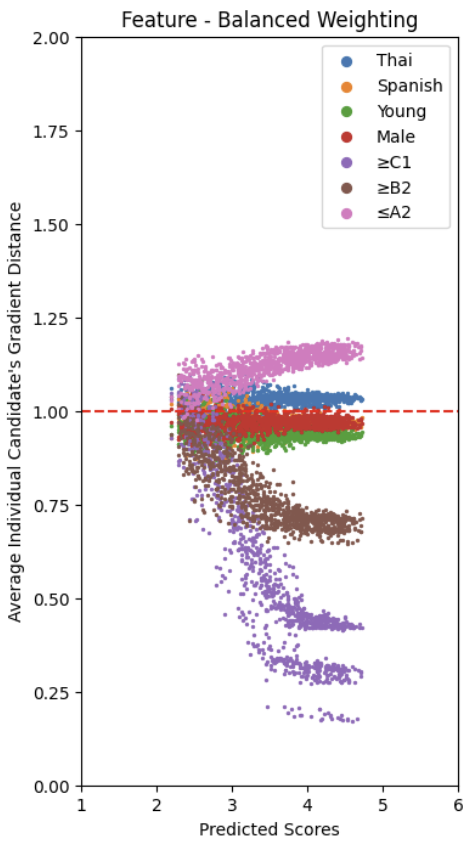
\includegraphics[width=0.48\linewidth]{feature_balanced.png}
        \hfill
        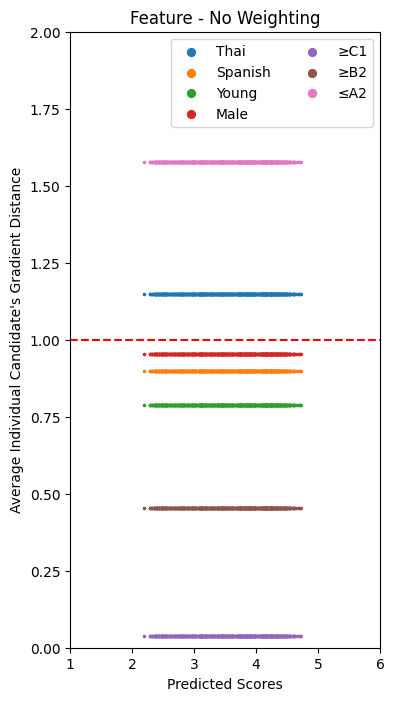
\includegraphics[width=0.48\linewidth]{feature_none.png}
        \caption{$\mathcal{B}^{(ci)}_{gr}$ for feature-based model}
        \label{fig:gradient_distance_feature}
    \end{minipage}
    \hfill
    \begin{minipage}[t]{0.48\textwidth}
        \centering
        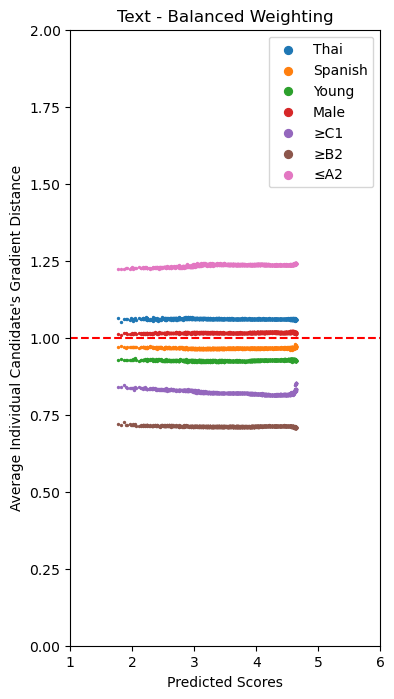
\includegraphics[width=0.48\linewidth]{text_balanced.png}
        \hfill
        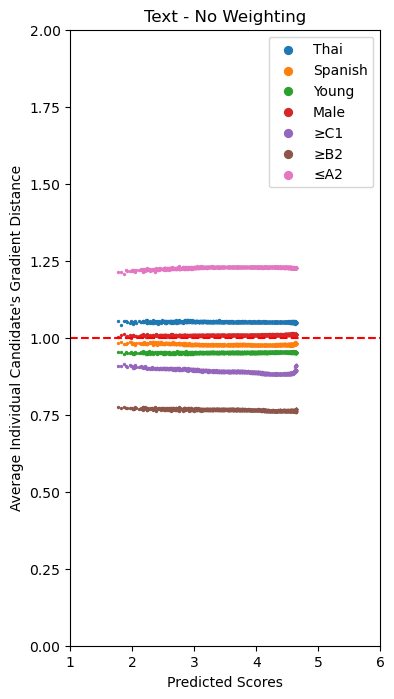
\includegraphics[width=0.48\linewidth]{text_none.png}
        \caption{$\mathcal{B}^{(ci)}_{gr}$ for text-based model}
        \label{fig:gradient_distance_text}
    \end{minipage}
    \hfill
    \begin{minipage}[t]{0.48\textwidth}
        \centering
        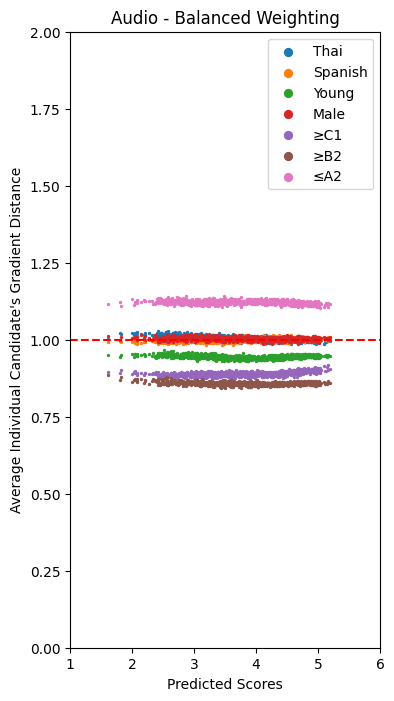
\includegraphics[width=0.48\linewidth]{audio_balanced.png}
        \hfill
        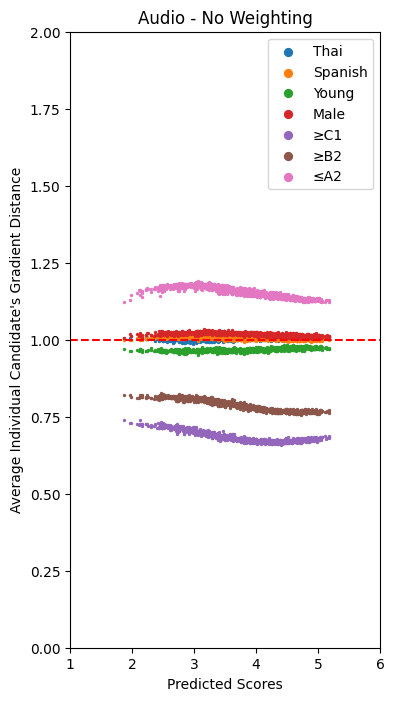
\includegraphics[width=0.48\linewidth]{audio_none.png}
        \caption{$\mathcal{B}^{(ci)}_{gr}$ for audio-based model}
        \label{fig:gradient_distance_audio}
    \end{minipage}
\end{figure}

% \begin{figure}[H]
%     \centering
%     \begin{minipage}[t]{0.32\textwidth}
%         \centering
%         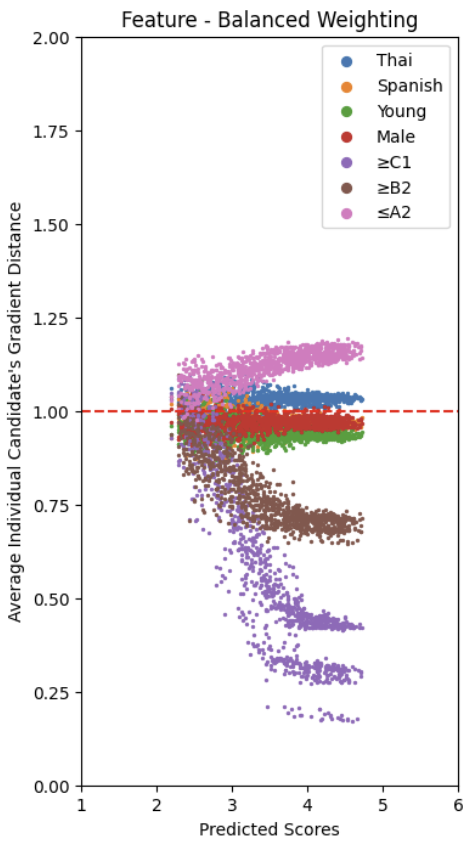
\includegraphics[width=0.48\linewidth]{feature_balanced.png}
%         \hfill
%         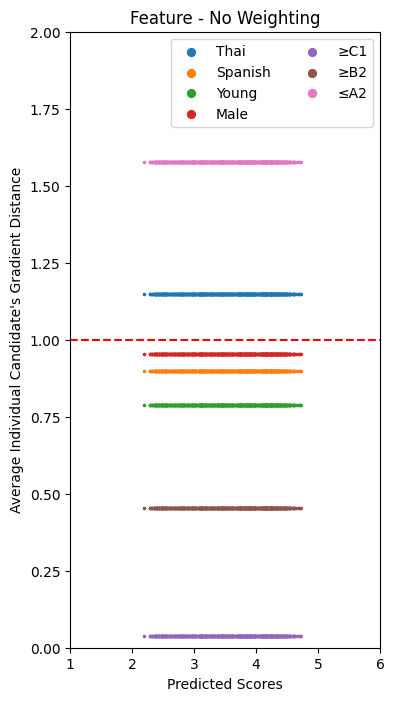
\includegraphics[width=0.48\linewidth]{feature_none.png}
%         \caption{$\mathcal{B}^{(ci)}_{gr}$ for feature-based model}
%         \label{fig:gradient_distance_feature}
%     \end{minipage}
%     \hfill
%     \begin{minipage}[t]{0.32\textwidth}
%         \centering
%         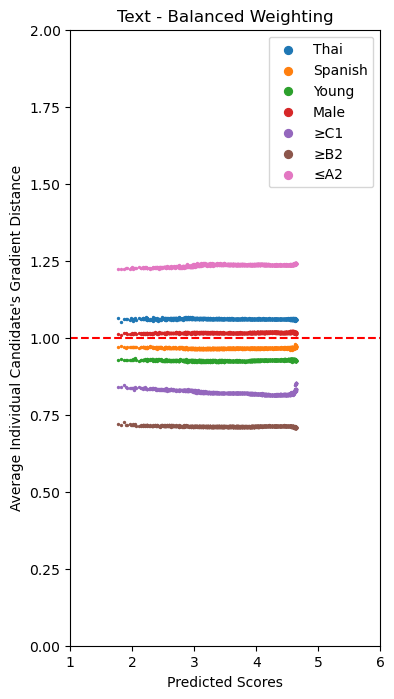
\includegraphics[width=0.48\linewidth]{text_balanced.png}
%         \hfill
%         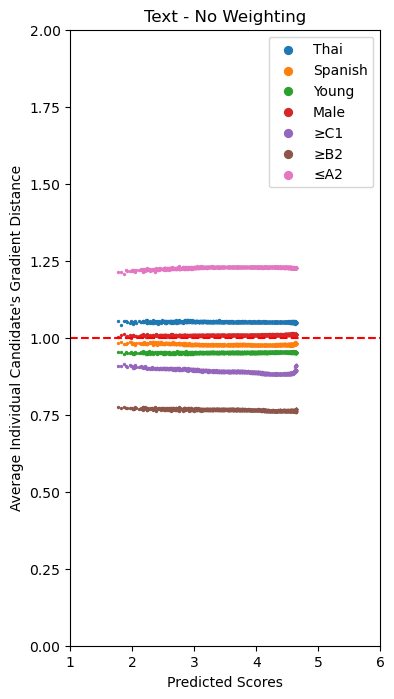
\includegraphics[width=0.48\linewidth]{text_none.png}
%         \caption{$\mathcal{B}^{(ci)}_{gr}$ for text-based model}
%         \label{fig:gradient_distance_text}
%     \end{minipage}
% \end{figure}

% \begin{figure}[H]
%     \centering
%     \resizebox{0.5\textwidth}{!}{
%         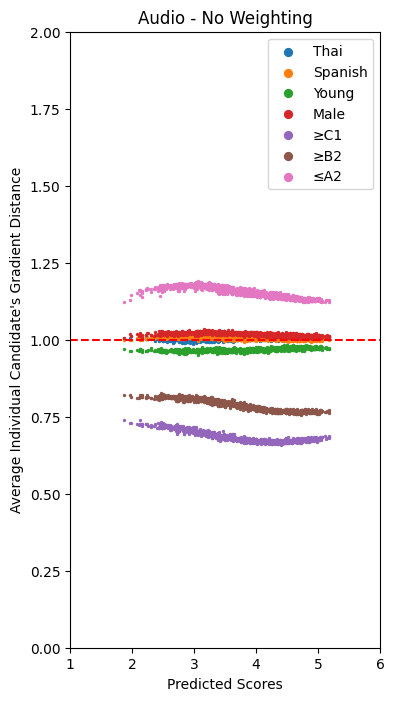
\includegraphics[width=0.48\linewidth]{audio_none.png}
%         \hfill
%         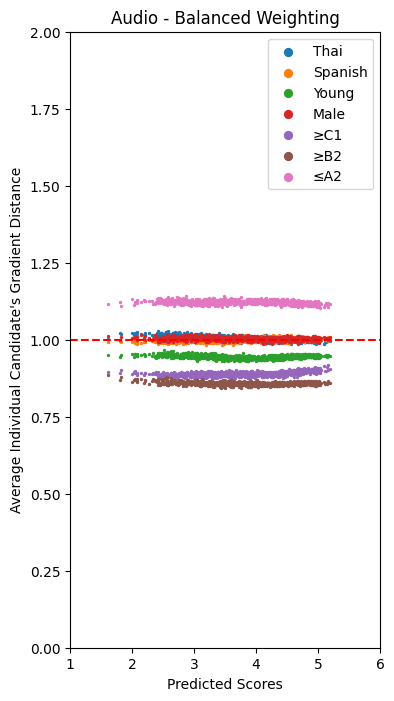
\includegraphics[width=0.48\linewidth]{audio_balanced.png}
%     }
%     \caption{$\mathcal{B}^{(ci)}_{gr}$ for audio-based model}
%     \label{fig:gradient_distance_audio}
% \end{figure}

The results are consistent with the findings from Table \ref{tab:gradient_distance_combined}. The non-grade concepts are close to 1, the `$\leq$ A2' concept is higher than 1, and the `$\geq$ B2' and `$\geq$ C1' concepts are lower than one. The pattern between those from no weighting and balanced weighting is similar. Also, feature-based model has the greatest deviation from 1 for all concepts.

All three graphs consist of a thin, horizontal lines, which shows that the bias measurement of the model is constant across different candidates with different predicted scores. The pattern from feature-based model differs from the pattern in Xizi's paper \cite{feature_bias}, which shows a thicker line with varying $\mathcal{B}^{(ci)}_{gr}$.'s value. However, the pattern extracted from the feature-based model, using the gradient before passing through the activation function, is more similar to the pattern in Xizi's paper (refer to Appendix \ref{app:feature_bias} for the comparison). It is possible that the extract in \cite{feature_bias} are in fact the pre-activation values.

Overall, this section shows that the three models are able to detect the bias from grade-related concepts, with feature-based model being the most sensitive to bias measurement. The CAV accuracy and the use of balanced weighting does not affect the sensitivity to bias measurement. The subsequent results in this chapter are then only presented for CAVs extracted with balanced weighting.

\subsection{Model Biasing} \label{sec:model_biasing}
The results in the previous section (Section \ref{sec:gradient_distance}) show that the three models are able to detect the bias from grade-related concepts. However, for non-grade related concepts, it is unsure whether the models are unbiased towards those concepts, or the CAVs are not able to detect the bias. To further investigate this, models biased towards the non-grade concepts (Thai, Spanish, Young, Male) are trained.

For each biased model, the CAV are used to detected the bias for the concept being biased through computing $\mathcal{B}^{(ci)}_{gr}$. The plot of $\mathcal{B}^{(ci)}_{gr}$ against candidates’ ensemble predicted score of the biased concepts are shown in Figure \ref{fig:grad_spanish_balanced} to \ref{fig:grad_young_balanced}, comparing the results with the original model without biasing.
\begin{figure}[H]
    \centering
    % Spanish
    \begin{subfigure}{0.32\textwidth}
        \centering
        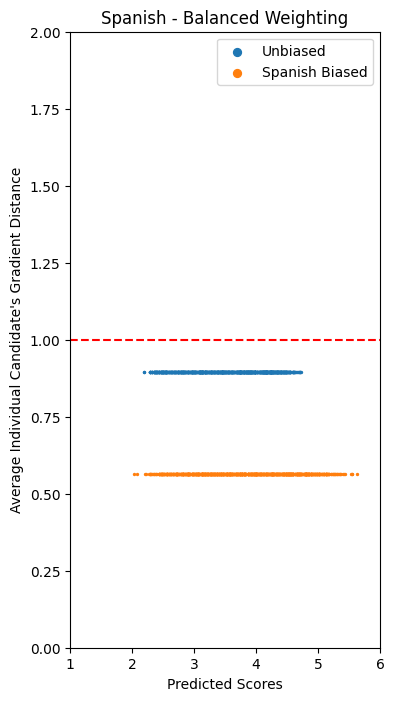
\includegraphics[width=0.7\linewidth]{Feature/spanish_part1_input_layer_balanced.png}
    \end{subfigure}
    \hfill
    \begin{subfigure}{0.32\textwidth}
        \centering
        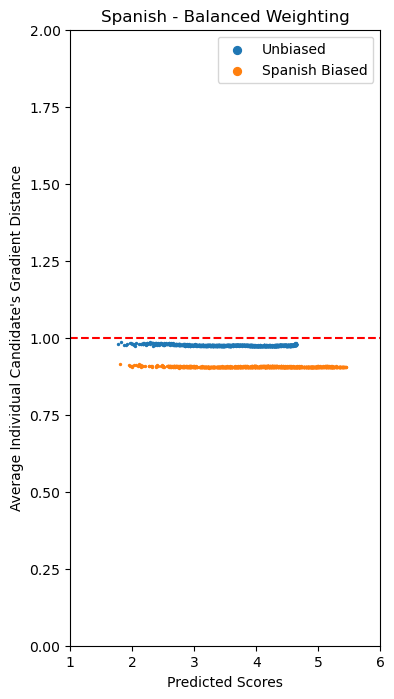
\includegraphics[width=0.7\linewidth]{Text/spanish_part1_layer1_balanced.png}
    \end{subfigure}
    \hfill
    \begin{subfigure}{0.32\textwidth}
        \centering
        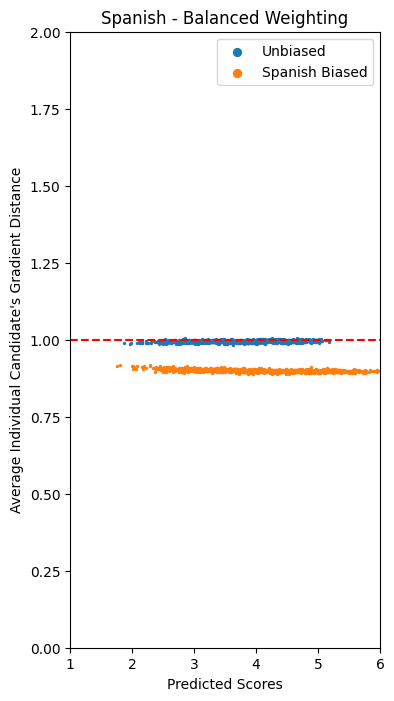
\includegraphics[width=0.7\linewidth]{Audio/spanish_part1_dense_balanced.png}
    \end{subfigure}
    \caption{$\mathcal{B}^{(ci)}_{gr}$ for Spanish concept for feature, text and audio-based model, left to right}
    \label{fig:grad_spanish_balanced}
\end{figure}

\begin{figure}[H]
    \centering
    % Thai
    \begin{subfigure}{0.32\textwidth}
        \centering
        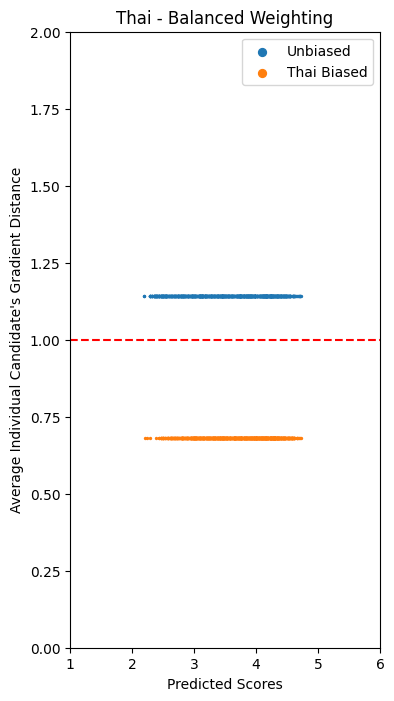
\includegraphics[width=0.7\linewidth]{Feature/thai_part1_input_layer_balanced.png}
    \end{subfigure}
    \hfill
    \begin{subfigure}{0.32\textwidth}
        \centering
        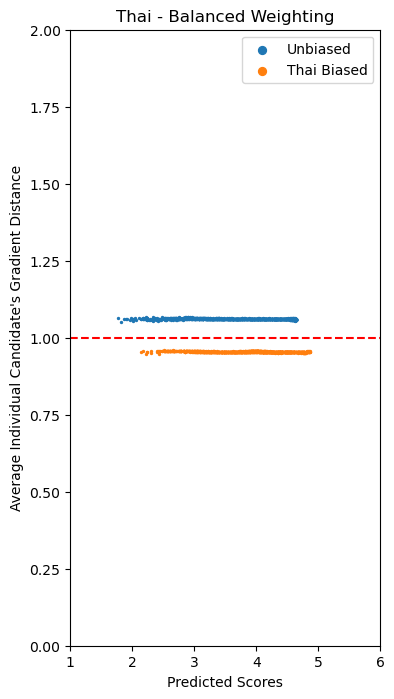
\includegraphics[width=0.7\linewidth]{Text/thai_part1_layer1_balanced.png}
    \end{subfigure}
    \hfill
    \begin{subfigure}{0.32\textwidth}
        \centering
        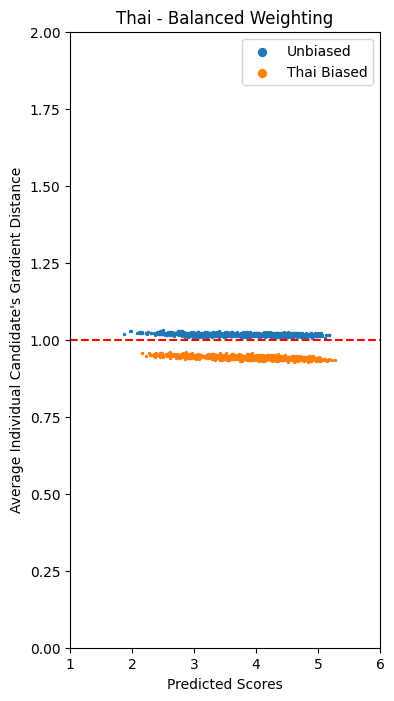
\includegraphics[width=0.7\linewidth]{Audio/thai_part1_dense_balanced.png}
    \end{subfigure}
    \caption{$\mathcal{B}^{(ci)}_{gr}$ for Thai concept for feature, text and audio-based model, left to right}
    \label{fig:grad_thai_balanced}
\end{figure}

\begin{figure}[H]
    \centering
    % Male
    \begin{subfigure}{0.32\textwidth}
        \centering
        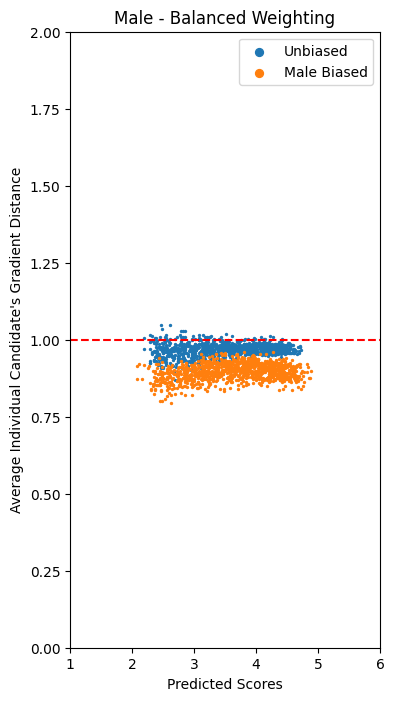
\includegraphics[width=0.7\linewidth]{Feature/male_part1_input_layer_balanced.png}
    \end{subfigure}
    \hfill
    \begin{subfigure}{0.32\textwidth}
        \centering
        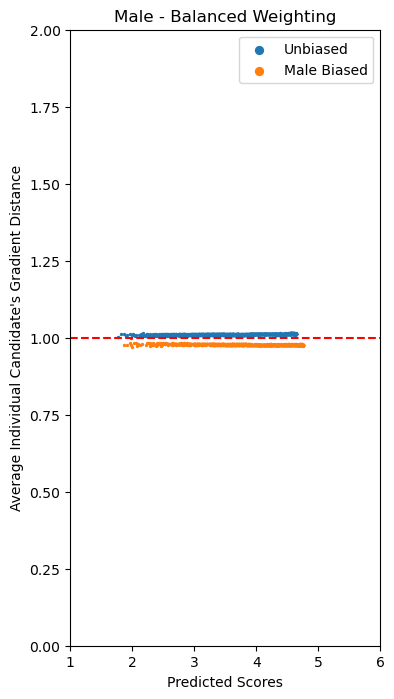
\includegraphics[width=0.7\linewidth]{Text/male_part1_layer1_balanced.png}
    \end{subfigure}
    \hfill
    \begin{subfigure}{0.32\textwidth}
        \centering
        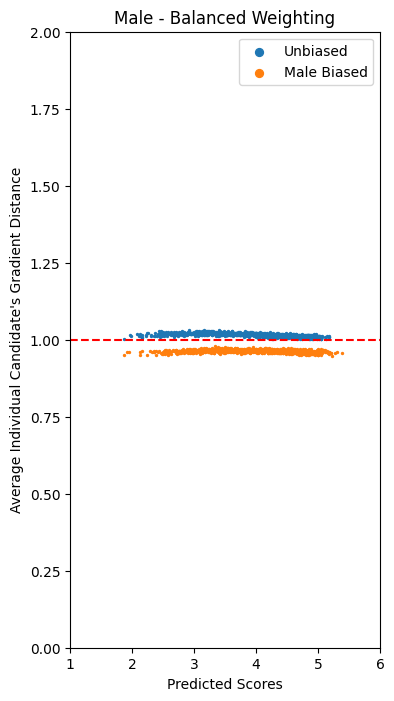
\includegraphics[width=0.7\linewidth]{Audio/male_part1_dense_balanced.png}
    \end{subfigure}
    \caption{$\mathcal{B}^{(ci)}_{gr}$ for Male concept for feature, text and audio-based model, left to right}
    \label{fig:grad_male_balanced}
\end{figure}

\begin{figure}[H]
    \centering
    % Young
    \begin{subfigure}{0.32\textwidth}
        \centering
        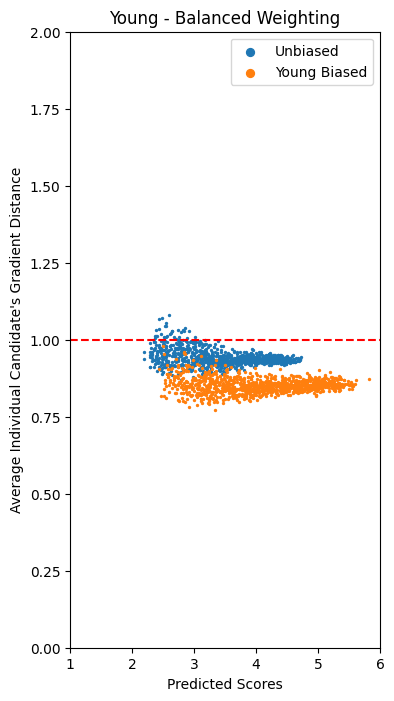
\includegraphics[width=0.7\linewidth]{Feature/young_part1_input_layer_balanced.png}
    \end{subfigure}
    \hfill
    \begin{subfigure}{0.32\textwidth}
        \centering
        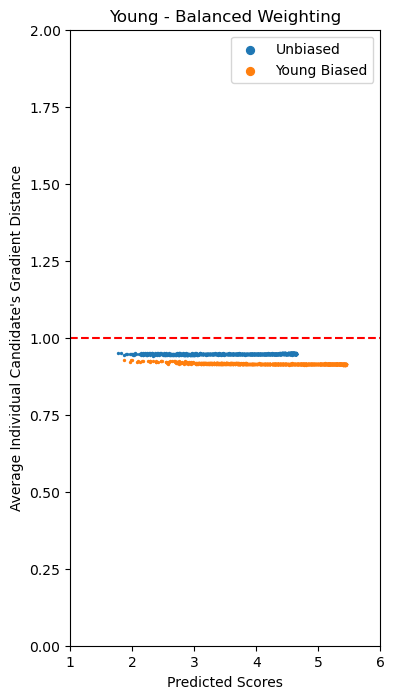
\includegraphics[width=0.7\linewidth]{Text/young_part1_layer1_balanced.png}
    \end{subfigure}
    \hfill
    \begin{subfigure}{0.32\textwidth}
        \centering
        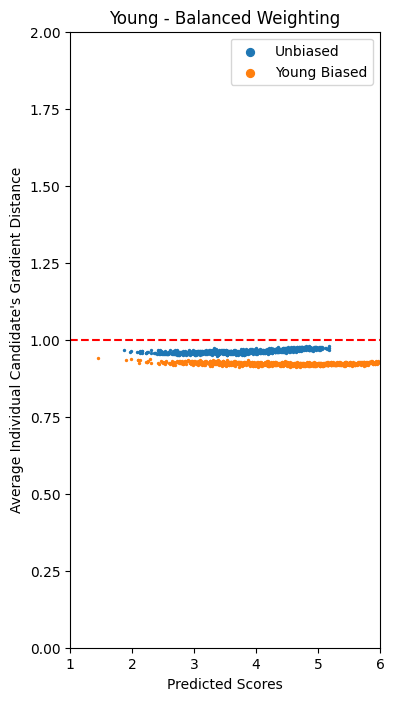
\includegraphics[width=0.7\linewidth]{Audio/young_part1_dense_balanced.png}
    \end{subfigure}
    \caption{$\mathcal{B}^{(ci)}_{gr}$ for Young concept for feature, text and audio-based model, left to right}
    \label{fig:grad_young_balanced}
\end{figure}

% \begin{figure}[H]
%     \centering
%     % First pair
%     \begin{minipage}[t]{0.48\textwidth}
%         \centering
%         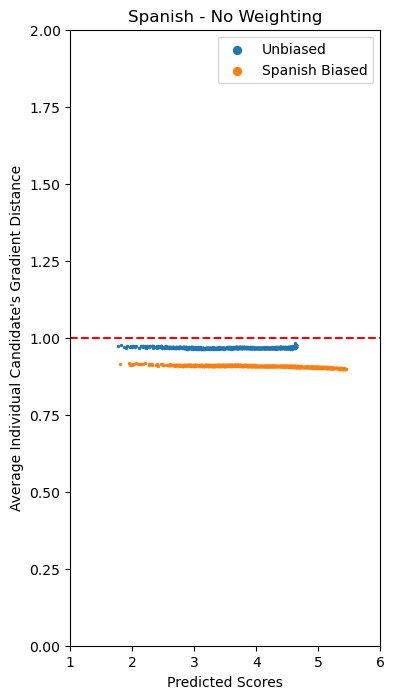
\includegraphics[width=0.32\linewidth]{Text/spanish_part1_layer1.png}
%         \hfill
%         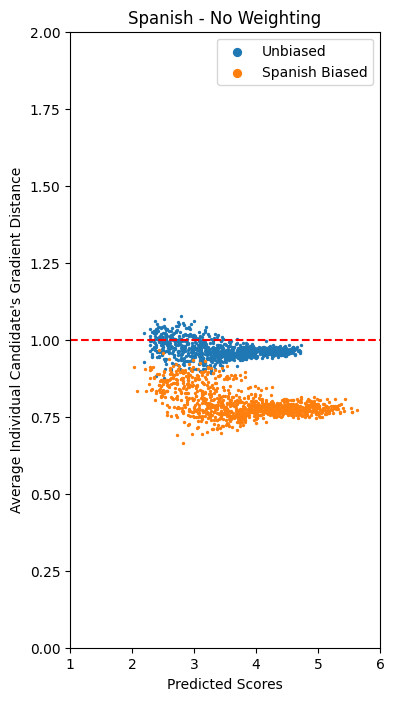
\includegraphics[width=0.32\linewidth]{Feature/spanish_part1_input_layer.png}
%         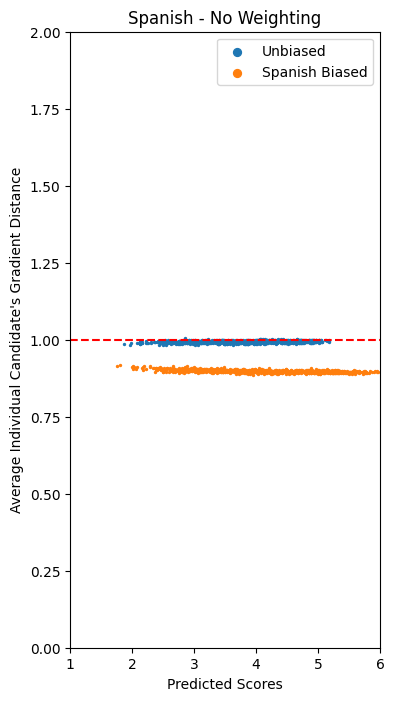
\includegraphics[width=0.32\linewidth]{Audio/spanish_part1_dense.png}
%         \caption{$\mathcal{B}^{(ci)}_{gr}$ for spanish concept across text, feature and audio-based model (left to right), no weighting}
%         \label{fig:grad_spanish}
%     \end{minipage}
%     \hfill
%     % Second pair
%     \begin{minipage}[t]{0.48\textwidth}
%         \centering
%         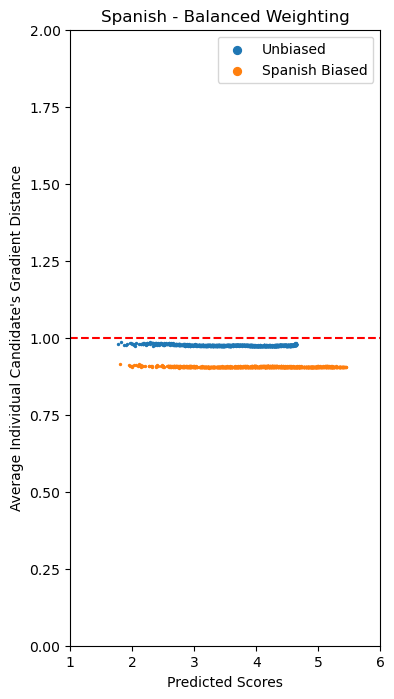
\includegraphics[width=0.32\linewidth]{Text/spanish_part1_layer1_balanced.png}
%         \hfill
%         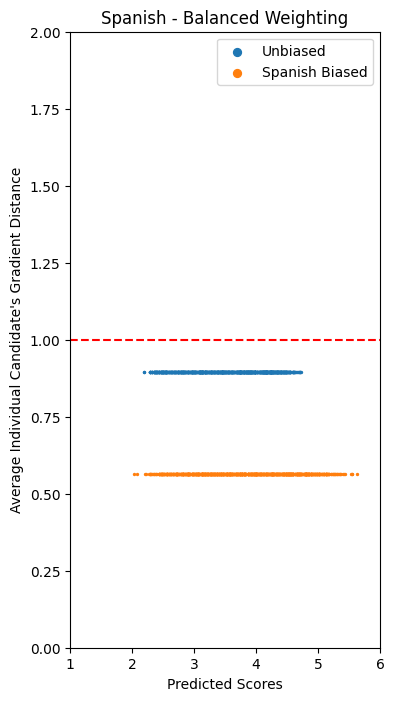
\includegraphics[width=0.32\linewidth]{Feature/spanish_part1_input_layer_balanced.png}
%         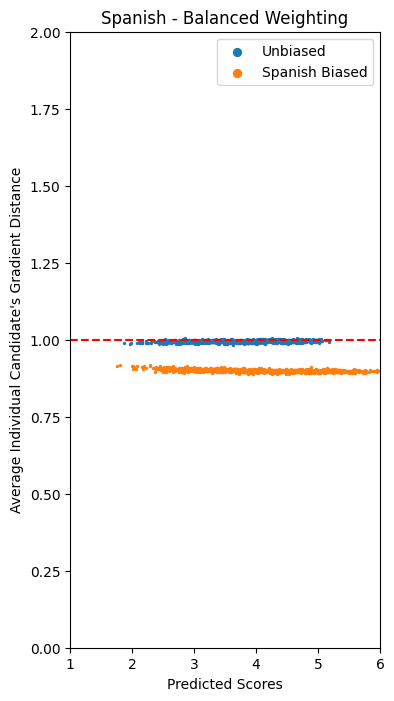
\includegraphics[width=0.32\linewidth]{Audio/spanish_part1_dense_balanced.png}
%         \caption{$\mathcal{B}^{(ci)}_{gr}$ for spanish concept across text, feature and audio-based model (left to right), balanced weighting}
%         \label{fig:grad_spanish_balanced}
%     \end{minipage}
% \end{figure}

% \begin{figure}[H]
%     \centering
%     % First pair
%     \begin{minipage}[t]{0.48\textwidth}
%         \centering
%         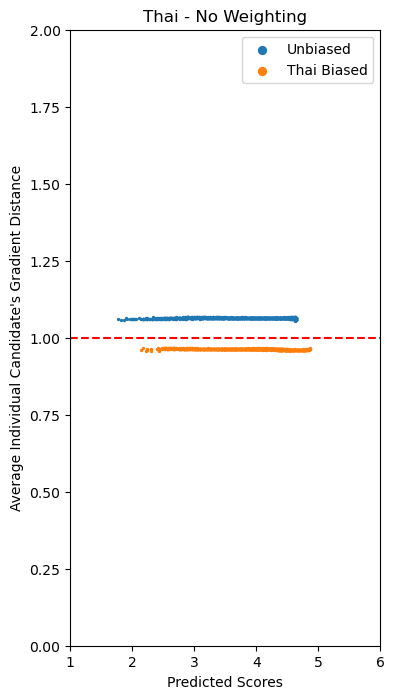
\includegraphics[width=0.32\linewidth]{Text/thai_part1_layer1.png}
%         \hfill
%         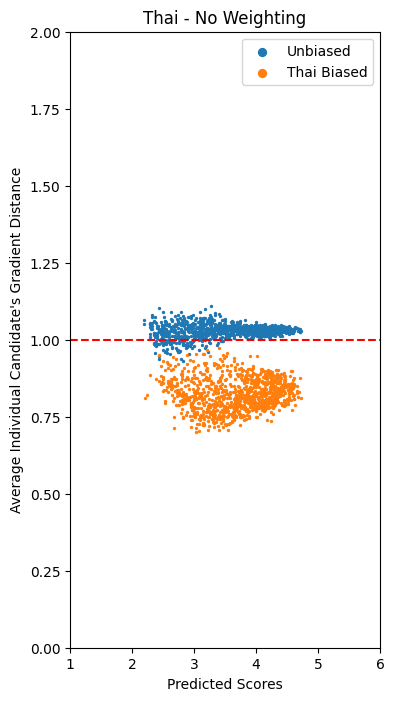
\includegraphics[width=0.32\linewidth]{Feature/thai_part1_input_layer.png}
%         \includegraphics[width=0.32\linewidth]{Audio/thai_part1_dense.png}
%         \caption{$\mathcal{B}^{(ci)}_{gr}$ for thai concept across text, feature and audio-based model (left to right), no weighting}
%         \label{fig:grad_thai}
%     \end{minipage}
%     \hfill
%     % Second pair
%     \begin{minipage}[t]{0.48\textwidth}
%         \centering
%         \includegraphics[width=0.32\linewidth]{Text/thai_part1_layer1_balanced.png}
%         \hfill
%         \includegraphics[width=0.32\linewidth]{Feature/thai_part1_input_layer_balanced.png}
%         \includegraphics[width=0.32\linewidth]{Audio/thai_part1_dense_balanced.png}
%         \caption{$\mathcal{B}^{(ci)}_{gr}$ for thai concept across text, feature and audio-based model (left to right), balanced weighting}
%         \label{fig:grad_thai_balanced}
%     \end{minipage}
% \end{figure}

% \begin{figure}[H]
%     \centering
%     % First pair
%     \begin{minipage}[t]{0.48\textwidth}
%         \centering
%         \includegraphics[width=0.32\linewidth]{Text/male_part1_layer1.png}
%         \hfill
%         \includegraphics[width=0.32\linewidth]{Feature/male_part1_input_layer.png}
%         \includegraphics[width=0.32\linewidth]{Audio/male_part1_dense.png}
%         \caption{$\mathcal{B}^{(ci)}_{gr}$ for male concept across text, feature and audio-based model (left to right), no weighting}
%         \label{fig:grad_male}
%     \end{minipage}
%     \hfill
%     % Second pair
%     \begin{minipage}[t]{0.48\textwidth}
%         \centering
%         \includegraphics[width=0.32\linewidth]{Text/male_part1_layer1_balanced.png}
%         \hfill
%         \includegraphics[width=0.32\linewidth]{Feature/male_part1_input_layer_balanced.png}
%         \includegraphics[width=0.32\linewidth]{Audio/male_part1_dense_balanced.png}
%         \caption{$\mathcal{B}^{(ci)}_{gr}$ for male concept across text, feature and audio-based model (left to right), balanced weighting}
%         \label{fig:grad_male_balanced}
%     \end{minipage}
% \end{figure}

% \begin{figure}[H]
%     \centering
%     % First pair
%     \begin{minipage}[t]{0.48\textwidth}
%         \centering
%         \includegraphics[width=0.32\linewidth]{Text/young_part1_layer1.png}
%         \hfill
%         \includegraphics[width=0.32\linewidth]{Feature/young_part1_input_layer.png}
%         \includegraphics[width=0.32\linewidth]{Audio/young_part1_dense.png}
%         \caption{$\mathcal{B}^{(ci)}_{gr}$ for young concept across text, feature and audio-based model (left to right), no weighting}
%         \label{fig:grad_young}
%     \end{minipage}
%     \hfill
%     % Second pair
%     \begin{minipage}[t]{0.48\textwidth}
%         \centering
%         \includegraphics[width=0.32\linewidth]{Text/young_part1_layer1_balanced.png}
%         \hfill
%         \includegraphics[width=0.32\linewidth]{Feature/young_part1_input_layer_balanced.png}
%         \includegraphics[width=0.32\linewidth]{Audio/young_part1_dense_balanced.png}
%         \caption{$\mathcal{B}^{(ci)}_{gr}$ for young concept across text, feature and audio-based model (left to right), balanced weighting}
%         \label{fig:grad_young_balanced}
%     \end{minipage}
% \end{figure}

% \begin{figure}[H]
%     \centering
%     \begin{minipage}{0.23\textwidth}
%         \begin{figure}[H]
%             \centering
%             \includegraphics[width=0.9\textwidth]{Text/spanish_part1_layer1.png}
%         \end{figure}
%     \end{minipage}
%     \begin{minipage}{0.23\textwidth}
%         \begin{figure}[H]
%             \centering
%             \includegraphics[width=0.9\textwidth]{Text/thai_part1_layer1.png}
%         \end{figure}
%     \end{minipage}
%     \begin{minipage}{0.23\textwidth}
%         \begin{figure}[H]
%             \centering
%             \includegraphics[width=0.9\textwidth]{Text/male_part1_layer1.png}
%         \end{figure}
%     \end{minipage}
%     \begin{minipage}{0.23\textwidth}
%         \begin{figure}[H]
%             \centering
%             \includegraphics[width=0.9\textwidth]{Text/young_part1_layer1.png}
%         \end{figure}
%     \end{minipage}
%     \caption{$\mathcal{B}_{gr}^{(ci)}$ for text-based model with no weighting}
%     \label{fig:grad_text}
% \end{figure}

% \begin{figure}[H]
%     \centering
%     \begin{minipage}{0.23\textwidth}
%         \begin{figure}[H]
%             \centering
%             \includegraphics[width=0.9\textwidth]{Text/spanish_part1_layer1_balanced.png}
%         \end{figure}
%     \end{minipage}
%     \begin{minipage}{0.23\textwidth}
%         \begin{figure}[H]
%             \centering
%             \includegraphics[width=0.9\textwidth]{Text/thai_part1_layer1_balanced.png}
%         \end{figure}
%     \end{minipage}
%     \begin{minipage}{0.23\textwidth}
%         \begin{figure}[H]
%             \centering
%             \includegraphics[width=0.9\textwidth]{Text/male_part1_layer1_balanced.png}
%         \end{figure}
%     \end{minipage}
%     \begin{minipage}{0.23\textwidth}
%         \begin{figure}[H]
%             \centering
%             \includegraphics[width=0.9\textwidth]{Text/young_part1_layer1_balanced.png}
%         \end{figure}
%     \end{minipage}
%     \caption{$\mathcal{B}_{gr}^{(ci)}$ for text-based model with balanced weighting}
%     \label{fig:grad_text_balanced}
% \end{figure}

% \begin{figure}[H]
%     \centering
%     \begin{minipage}{0.23\textwidth}
%         \begin{figure}[H]
%             \centering
%             \includegraphics[width=0.9\textwidth]{Feature/spanish_part1_input_layer.png}
%         \end{figure}
%     \end{minipage}
%     \begin{minipage}{0.23\textwidth}
%         \begin{figure}[H]
%             \centering
%             \includegraphics[width=0.9\textwidth]{Feature/thai_part1_input_layer.png}
%         \end{figure}
%     \end{minipage}
%     \begin{minipage}{0.23\textwidth}
%         \begin{figure}[H]
%             \centering
%             \includegraphics[width=0.9\textwidth]{Feature/male_part1_input_layer.png}
%         \end{figure}
%     \end{minipage}
%     \begin{minipage}{0.23\textwidth}
%         \begin{figure}[H]
%             \centering
%             \includegraphics[width=0.9\textwidth]{Feature/young_part1_input_layer.png}
%         \end{figure}
%     \end{minipage}
%     \caption{$\mathcal{B}_{gr}^{(ci)}$ for feature-based model with no weighting}
%     \label{fig:grad_feature}
% \end{figure}

% \begin{figure}[H]
%     \centering
%     \begin{minipage}{0.23\textwidth}
%         \begin{figure}[H]
%             \centering
%             \includegraphics[width=0.9\textwidth]{Feature/spanish_part1_input_layer_balanced.png}
%         \end{figure}
%     \end{minipage}
%     \begin{minipage}{0.23\textwidth}
%         \begin{figure}[H]
%             \centering
%             \includegraphics[width=0.9\textwidth]{Feature/thai_part1_input_layer_balanced.png}
%         \end{figure}
%     \end{minipage}
%     \begin{minipage}{0.23\textwidth}
%         \begin{figure}[H]
%             \centering
%             \includegraphics[width=0.9\textwidth]{Feature/male_part1_input_layer_balanced.png}
%         \end{figure}
%     \end{minipage}
%     \begin{minipage}{0.23\textwidth}
%         \begin{figure}[H]
%             \centering
%             \includegraphics[width=0.9\textwidth]{Feature/young_part1_input_layer_balanced.png}
%         \end{figure}
%     \end{minipage}
%     \caption{$\mathcal{B}_{gr}^{(ci)}$ for feature-based model with balanced weighting}
%     \label{fig:grad_feature_balanced}
% \end{figure}

% \begin{figure}[H]
%     \centering
%     \begin{minipage}{0.23\textwidth}
%         \begin{figure}[H]
%             \centering
%             \includegraphics[width=0.9\textwidth]{Audio/spanish_part1_dense.png}
%         \end{figure}
%     \end{minipage}
%     \begin{minipage}{0.23\textwidth}
%         \begin{figure}[H]
%             \centering
%             \includegraphics[width=0.9\textwidth]{Audio/thai_part1_dense.png}
%         \end{figure}
%     \end{minipage}
%     \begin{minipage}{0.23\textwidth}
%         \begin{figure}[H]
%             \centering
%             \includegraphics[width=0.9\textwidth]{Audio/male_part1_dense.png}
%         \end{figure}
%     \end{minipage}
%     \begin{minipage}{0.23\textwidth}
%         \begin{figure}[H]
%             \centering
%             \includegraphics[width=0.9\textwidth]{Audio/young_part1_dense.png}
%         \end{figure}
%     \end{minipage}
%     \caption{$\mathcal{B}_{gr}^{(ci)}$ for text-based model with no weighting}
%     \label{fig:grad_audio}
% \end{figure}

% \begin{figure}[H]
%     \centering
%     \begin{minipage}{0.23\textwidth}
%         \begin{figure}[H]
%             \centering
%             \includegraphics[width=0.9\textwidth]{Audio/spanish_part1_dense_balanced.png}
%         \end{figure}
%     \end{minipage}
%     \begin{minipage}{0.23\textwidth}
%         \begin{figure}[H]
%             \centering
%             \includegraphics[width=0.9\textwidth]{Audio/thai_part1_dense_balanced.png}
%         \end{figure}
%     \end{minipage}
%     \begin{minipage}{0.23\textwidth}
%         \begin{figure}[H]
%             \centering
%             \includegraphics[width=0.9\textwidth]{Audio/male_part1_dense_balanced.png}
%         \end{figure}
%     \end{minipage}
%     \begin{minipage}{0.23\textwidth}
%         \begin{figure}[H]
%             \centering
%             \includegraphics[width=0.9\textwidth]{Audio/young_part1_dense_balanced.png}
%         \end{figure}
%     \end{minipage}
%     \caption{$\mathcal{B}_{gr}^{(ci)}$ for audio-based model with balanced weighting}
%     \label{fig:grad_audio_balanced}
% \end{figure}

The results from model biasing is aligned with the results found in Section \ref{sec:gradient_distance}. As before, it is observed that the pattern of $\mathcal{B}^{(ci)}_{gr}$ between graphs without weighting and balanced weighting is similar. This indicates that either method is able to detect the bias equally for the concepts.

In addition, aligning with previous results, the change in $\mathcal{B}^{(ci)}_{gr}$ for the feature-based model is more significant than the text-based and audio-based models, with the gap of $\mathcal{B}^{(ci)}_{gr}$ between the original and bias models being the widest. This verifies that the feature-based model is more sensitive to the bias presence, such that the CAVs are able to detect the bias presence better.

It is found that CAV are more sensitive to L1-related biases. From the figures, the change in $\mathcal{B}^{(ci)}_{gr}$ within L1-related concepts (Thai, Spanish), particularly Spanish, is more significant compared to other concepts across all three models. For non-L1 concepts (Male, Young), the change is negligible in text and audio-based models, hence the CAVs are actually unable to detect biases presence for those concepts. It is interesting to observe that the text-based model has its $\mathcal{B}^{(ci)}_{gr}$ deviating more from 1 for the original model than the biased version, which might indicate the initial model has slight bias towards Thai speaker. Regardless, the results reflect that CAVs are better in detecting bias presence for L1-related concepts than non-L1 concepts in these models.

The result further supports the lack of correlation between CAV accuracy and sensitivity to bias presence. From Table \ref{tab:CAV_accuracy_combined}, the CAV accuracy for audio-based model is the highest, yet it is much less sensitive than feature-based model in detecting bias presence. In contrast, L1-related (Thai, Spanish) CAV has a higher CAV accuracy, and the result does show that CAVs are generally more sensitive to biases in L1-related concepts.

Overall, this shows that CAV can best detect bias towards L1-concepts, particularly Spanish L1-speaker in feature-based models compared to other concepts and models. It is unable to detect non-L1 related biases in text and audio-based models. It also supports the finding in Section \ref{sec:gradient_distance} that CAV accuracy and the use of balanced weighting does not affect the sensitivity to bias measurement.

\section{Factor Isolation} \label{sec:factor_isolation}
This section presents the result of the experiments performed on the modified models to isolate the effect of different factors on the bias measurement. The previous section (Section \ref{sec:bias_detection}) shows that plots of $\mathcal{B}^{(ci)}_{gr}$ against ensemble score for feature-based model spans wider than text and audio based model. The models differ in network architecture, model type, activation function, and input type, which are all possible factors that could influence $\mathcal{B}^{(ci)}_{gr}$'s pattern. Hence, they are evaluated to uncover the factors affecting the pattern. The results are compared with the original models to see the changes in pattern. All the CAVs are extracted with balanced weighting.

\subsection{Network Architecture} \label{sec:network_architecture}
The first experiment changes the network of the feature-based model to the network from the text-based model (Figure \ref{fig:bert_like}). The changes including the node and layer number, and dropout rate, with the feature vector retained as input, and activation function kept as LReLU. This is to see if the architecture of the network affects the bias measurement.

The accuracy of the modified feature-based model is compared with the original feature-based model, as shown in Table \ref{tab:model_accuracy_bert_like}. The coefficients for the linear calibration of both models are presented in Table \ref{tab:linear_regression_coefficients_bert_like} as a reference. The results show that the modified model is decent and even perform slightly better than the original feature-based model, indicating that the architecture change does not affect the model performance significantly, hence reliable for CAV extraction.

\begin{table}[H]
    \centering
    \begin{tabular}{|lc|c|c|c|c|}
        \hline
        \multicolumn{2}{|l|}{\textbf{}}                                         & \textbf{RMSE}         & \textbf{PCC} & \textbf{\textless 0.5} & \textbf{\textless 1}        \\ \hline
        \multicolumn{1}{|l|}{\multirow{2}{*}{\textbf{Original Architecture}}}   & \textbf{Uncalibrated} & 0.694        & 0.821                  & 55.3                 & 83.4 \\ \cline{2-6}
        \multicolumn{1}{|l|}{}                                                  & \textbf{Calibrated}   & 0.638        & 0.821                  & 56.6                 & 87.9 \\ \hline
        \multicolumn{1}{|l|}{\multirow{2}{*}{\textbf{Text-based Architecture}}} & \textbf{Uncalibrated} & 0.670        & 0.826                  & 57.2                 & 86.6 \\ \cline{2-6}
        \multicolumn{1}{|l|}{}                                                  & \textbf{Calibrated}   & 0.631        & 0.826                  & 59.5                 & 88.5 \\ \hline
    \end{tabular}
    \caption{Model accuracy for the feature-based model with the original and text-based network architecture, both calibrated and uncalibrated.}
    \label{tab:model_accuracy_bert_like}
\end{table}


\begin{table}[H]
    \centering
    \begin{tabular}{|l|c|c|}
        \hline
        \textbf{}                        & \textbf{Slope (m)} & \textbf{Intercept (c)} \\ \hline
        \textbf{Original Architecture}   & 1.42               & -1.45                  \\ \hline
        \textbf{Text-based Architecture} & 1.32               & -1.16                  \\ \hline
    \end{tabular}
    \caption{Linear calibration coefficients for the feature-based model with the original and text-based network architecture}
    \label{tab:linear_regression_coefficients_bert_like}
\end{table}

The accuracy of the CAVs extracted from the modified feature-based model is shown in Table \ref{tab:CAV_accuracy_bert_like}. The results show that the CAVs from the modified model are able to differentiate the positive and negative targets with reasonable accuracy, and in fact slightly better than the original feature-based model. Hence, it could be used to measure bias reliably.

\begin{table}[H]
    \centering
    \begin{tabular}{|c|cc|cc|}
        \hline
        \multirow{2}{*}{\textbf{Concept}}
                  & \multicolumn{2}{c|}{\shortstack{\textbf{Original}                                        \\ \textbf{Architecture}}}
                  & \multicolumn{2}{c|}{\shortstack{\textbf{Text-based}                                      \\ \textbf{Architecture}}} \\ \cline{2-5}
                  & \multicolumn{1}{c|}{\textbf{+ve}}                   & \textbf{-ve}
                  & \multicolumn{1}{c|}{\textbf{+ve}}                   & \textbf{-ve}                       \\ \hline

        $\geq$ C1 & \multicolumn{1}{c|}{$94.0_{\pm 0.5}$}               & $76.9_{\pm 1.8}$
                  & \multicolumn{1}{c|}{$95.5_{\pm 0.6}$}               & $85.3_{\pm 1.1}$                   \\

        $\geq$ B2 & \multicolumn{1}{c|}{$86.0_{\pm 0.2}$}               & $76.5_{\pm 0.6}$
                  & \multicolumn{1}{c|}{$85.2_{\pm 0.1}$}               & $81.2_{\pm 0.2}$                   \\

        $\leq$ A2 & \multicolumn{1}{c|}{$81.5_{\pm 0.2}$}               & $79.3_{\pm 0.2}$
                  & \multicolumn{1}{c|}{$86.2_{\pm 0.2}$}               & $79.4_{\pm 0.3}$                   \\  \hline

        Thai      & \multicolumn{1}{c|}{$82.9_{\pm 0.9}$}               & $82.4_{\pm 0.5}$
                  & \multicolumn{1}{c|}{$91.8_{\pm 0.2}$}               & $88.3_{\pm 0.3}$                   \\

        Spanish   & \multicolumn{1}{c|}{$83.7_{\pm 0.4}$}               & $73.6_{\pm 0.1}$
                  & \multicolumn{1}{c|}{$85.4_{\pm 0.2}$}               & $89.1_{\pm 0.2}$                   \\  \hline

        Young     & \multicolumn{1}{c|}{$74.0_{\pm 0.5}$}               & $\cellcolor{red!15}56.4_{\pm 0.3}$
                  & \multicolumn{1}{c|}{$71.9_{\pm 0.3}$}               & $69.1_{\pm 0.5}$                   \\

        Male      & \multicolumn{1}{c|}{$61.7_{\pm 0.7}$}               & $65.2_{\pm 0.9}$
                  & \multicolumn{1}{c|}{$73.9_{\pm 0.5}$}               & $73.2_{\pm 0.5}$                   \\ \hline
    \end{tabular}
    \caption{Accuracy of CAV in differentiating positive and negative training data for the feature-based model with the original and text-based network architecture. Range indicates $\pm \sigma$.}
    \label{tab:CAV_accuracy_bert_like}
\end{table}

Finally, Figure \ref{fig:gradient_distance_bert_like_original} and \ref{fig:gradient_distance_bert_like_modified} compare the changes of $\mathcal{B}^{(ci)}_{gr}$ against predicted ensemble score for the original and modified feature-based model with text-based architecture, respectively. The values of $\mathcal{B}^{(ci)}_{gr}$ are still relatively flat, although the left side is slightly thicker, implying the network has some effect to the pattern thickness. $\mathcal{B}^{(ci)}_{gr}$ are still widespread across the range of gradient distance, although less than the original pattern. Particularly, C1's $\mathcal{B}^{(ci)}_{gr}$ being much closer to 1, meaning the C1's CAV is not as sensitive to the bias measurement. Hence, as the sensitivity has only changed slightly, the evidence is not strong enough to conclude that the network architecture affects the sensitivity bias measurement.

\begin{figure}[H]
    \centering
    % First pair
    \begin{minipage}[t]{0.48\textwidth}
        \centering
        \includegraphics[width=0.48\linewidth]{BERT-like/original_bias_part1_input_layer_balanced.png}
        \caption{$\mathcal{B}^{(ci)}_{gr}$ for feature-based model with original network architecture}
        \label{fig:gradient_distance_bert_like_original}
    \end{minipage}
    \hfill
    % Second pair
    \begin{minipage}[t]{0.48\textwidth}
        \centering
        \includegraphics[width=0.48\linewidth]{BERT-like/modified_bias_part1_input_layer_balanced.png}
        \caption{$\mathcal{B}^{(ci)}_{gr}$ for feature-based model with the text-based like network architecture}
        \label{fig:gradient_distance_bert_like_modified}
    \end{minipage}
\end{figure}

\subsection{Model Type}
The second experiment changes the feature-based model from DNN to DDN (Figure \ref{fig:dnn_like}). The loss function in training is subsequently updated from NLL to MSE. This is to see if the model type affects the bias measurement.

The accuracy of the modified feature-based model is compared with the original feature-based model, as shown in Table \ref{tab:model_accuracy_dnn_like}. The coefficients for the linear calibration of both models are presented in Table \ref{tab:linear_regression_coefficients_dnn_like} as a reference. The results show that the modified model is decent and even perform slightly better than the original feature-based model, indicating that the architecture change does not affect the model performance significantly, hence reliable for CAV extraction.

\begin{table}[H]
    \centering
    \begin{tabular}{|l|l|c|c|c|c|}
        \hline
        \multicolumn{2}{|l|}{\textbf{}} & \textbf{RMSE} & \textbf{PCC} & \textbf{\textless 0.5} & \textbf{\textless 1}          \\ \hline
        \multirow{2}{*}{\textbf{Original (DDN)}}
                                        & Uncalibrated  & $0.694$      & $0.821$                & $55.3$               & $83.4$ \\ \cline{2-6}
                                        & Calibrated    & $0.638$      & $0.821$                & $56.6$               & $87.9$ \\ \hline
        \multirow{2}{*}{\textbf{Modified (DNN)}}
                                        & Uncalibrated  & $0.688$      & $0.822$                & $55.2$               & $84.4$ \\ \cline{2-6}
                                        & Calibrated    & $0.637$      & $0.822$                & $57.1$               & $88.2$ \\ \hline
    \end{tabular}
    \caption{Model accuracy for the original (DDN) and modified (DNN) feature-based mode, both calibrated and uncalibrated.}
    \label{tab:model_accuracy_dnn_like}
\end{table}


\begin{table}[H]
    \centering
    \begin{tabular}{|l|c|c|}
        \hline
        \textbf{}               & \textbf{Slope (m)} & \textbf{Intercept (c)} \\ \hline
        \textbf{Original (DDN)} & $1.420$            & $-1.451$               \\ \hline
        \textbf{Modified (DNN)} & $1.393$            & $-1.392$               \\ \hline
    \end{tabular}
    \caption{Linear calibration coefficients for the original (DDN) and modified (DNN) feature-based model}
    \label{tab:linear_regression_coefficients_dnn_like}
\end{table}

The accuracy of the CAVs extracted from the modified feature-based model is shown in Table \ref{tab:CAV_accuracy_bert_like}. The results show that the CAVs from the modified DNN model have nearly identical performance as the original DDN model. Hence, it could be used to measure bias reliably.

\begin{table}[H]
    \centering
    \begin{tabular}{|c|cc|cc|}
        \hline
        \multirow{2}{*}{\textbf{Concept}}
                  & \multicolumn{2}{c|}{\shortstack{\textbf{Original}                                        \\ \textbf{(DDN)}}}
                  & \multicolumn{2}{c|}{\shortstack{\textbf{Modified}                                        \\ \textbf{(DNN)}}} \\ \cline{2-5}
                  & \multicolumn{1}{c|}{\textbf{+ve}}                 & \textbf{-ve}
                  & \multicolumn{1}{c|}{\textbf{+ve}}                 & \textbf{-ve}                         \\ \hline
        $\geq$ C1 & \multicolumn{1}{c|}{$94.0_{\pm 0.5}$}             & $76.9_{\pm 1.8}$
                  & \multicolumn{1}{c|}{$93.2_{\pm 1.0}$}             & $77.1_{\pm 1.2}$                     \\
        $\geq$ B2 & \multicolumn{1}{c|}{$86.0_{\pm 0.2}$}             & $76.5_{\pm 0.6}$
                  & \multicolumn{1}{c|}{$86.0_{\pm 0.1}$}             & $76.5_{\pm 0.6}$                     \\
        $\leq$ A2 & \multicolumn{1}{c|}{$81.5_{\pm 0.2}$}             & $79.3_{\pm 0.2}$
                  & \multicolumn{1}{c|}{$81.7_{\pm 0.2}$}             & $79.4_{\pm 0.2}$                     \\ \hline
        Thai      & \multicolumn{1}{c|}{$82.9_{\pm 0.9}$}             & $82.4_{\pm 0.5}$
                  & \multicolumn{1}{c|}{$83.3_{\pm 1.0}$}             & ${82.4_{\pm 0.5}}$                   \\
        Spanish   & \multicolumn{1}{c|}{$83.7_{\pm 0.4}$}             & ${73.6_{\pm 0.1}}$
                  & \multicolumn{1}{c|}{$83.6_{\pm 0.5}$}             & ${73.9_{\pm 1.0}}$                   \\ \hline
        Young     & \multicolumn{1}{c|}{$74.0_{\pm 0.5}$}             & $\cellcolor{red!15}{56.4_{\pm 0.3}}$
                  & \multicolumn{1}{c|}{$73.9_{\pm 0.3}$}             & $\cellcolor{red!15}{56.5_{\pm 0.2}}$ \\ \hline
        Male      & \multicolumn{1}{c|}{$61.7_{\pm 0.7}$}             & $65.2_{\pm 0.9}$
                  & \multicolumn{1}{c|}{$62.1_{\pm 0.4}$}             & $64.7_{\pm 1.0}$                     \\ \hline
    \end{tabular}
    \caption{Accuracy of CAV in differentiating positive and negative training data for the original (DDN) and modified (DNN) feature-based model. Range indicates $\pm \sigma$.}
    \label{tab:CAV_accuracy_dnn_like}
\end{table}

Finally, Figure \ref{fig:gradient_distance_dnn_like_original} and \ref{fig:gradient_distance_dnn_like_modified} compare the changes of $\mathcal{B}^{(ci)}_{gr}$ against predicted ensemble score for the original DDN and modified DNN feature-based model, respectively. The pattern are nearly identical, which concludes that the model type does not affect the gradient distance pattern.

\begin{figure}[H]
    \centering
    % First pair
    \begin{minipage}[t]{0.48\textwidth}
        \centering
        \includegraphics[width=0.48\linewidth]{DNN-like/DDN_bias_part1_input_layer_balanced.png}
        \caption{$\mathcal{B}^{(ci)}_{gr}$ for the original DDN feature-based model}
        \label{fig:gradient_distance_dnn_like_original}
    \end{minipage}
    \hfill
    % Second pair
    \begin{minipage}[t]{0.48\textwidth}
        \centering
        \includegraphics[width=0.48\linewidth]{DNN-like/DNN_bias_part1_input_layer_balanced.png}
        \caption{$\mathcal{B}^{(ci)}_{gr}$ for the modified DNN feature-based model}
        \label{fig:gradient_distance_dnn_like_modified}
    \end{minipage}
\end{figure}

\subsection{Feature Activation Function} \label{sec:feature_activation_function}
The third experiment changes the activation function of the feature-based model from LReLU to ReLU (Figure \ref{fig:relu}). This is to see if the activation function affects the bias measurement.

The accuracy of the ReLU feature-based model is compared with the LReLU feature-based model, as shown in Table \ref{tab:model_accuracy_relu}. The coefficients for the linear calibration of both models are presented in Table \ref{tab:linear_regression_coefficients_relu} as a reference. The results show that the modified model is decent, just perform slightly less accurate than the original feature-based model, indicating that the architecture change does not affect the model performance significantly, hence reliable for CAV extraction.

\begin{table}[H]
    \centering
    \begin{tabular}{|l|l|c|c|c|c|}
        \hline
        \multicolumn{2}{|l|}{\textbf{}} & \textbf{RMSE} & \textbf{PCC} & \textbf{\textless 0.5} & \textbf{\textless 1}          \\ \hline
        \multirow{2}{*}{\textbf{Original (LReLU)}}
                                        & Uncalibrated  & $0.694$      & $0.821$                & $55.3$               & $83.4$ \\ \cline{2-6}
                                        & Calibrated    & $0.638$      & $0.821$                & $56.6$               & $87.9$ \\ \hline
        \multirow{2}{*}{\textbf{Modified (ReLU)}}
                                        & Uncalibrated  & $0.715$      & $0.829$                & $51.8$               & $83.3$ \\ \cline{2-6}
                                        & Calibrated    & $0.625$      & $0.829$                & $59.8$               & $88.7$ \\ \hline
    \end{tabular}
    \caption{Model accuracy for the original (LReLU) and modified (ReLU) feature-based model, both calibrated and uncalibrated.}
    \label{tab:model_accuracy_relu}
\end{table}


\begin{table}[H]
    \centering
    \begin{tabular}{|l|c|c|}
        \hline
        \textbf{}                 & \textbf{Slope (m)} & \textbf{Intercept (c)} \\ \hline
        \textbf{Modified (ReLU)}  & $1.54$             & $-1.70$                \\ \hline
        \textbf{Original (LReLU)} & $1.420$            & $-1.451$               \\ \hline
    \end{tabular}
    \caption{Linear calibration coefficients for the modified (ReLU) and original (LReLU) feature-based model}
    \label{tab:linear_regression_coefficients_relu}
\end{table}

The accuracy of the CAVs extracted from the modified feature-based model is shown in Table \ref{tab:CAV_accuracy_relu}. The results show that the CAVs from the modified ReLU model have nearly identical performance as the original LReLU model. Hence, it could be used to measure bias reliably.
\begin{table}[H]
    \centering
    \begin{tabular}{|c|cc|cc|}
        \hline
        \multirow{2}{*}{\textbf{Concept}}
                  & \multicolumn{2}{c|}{\textbf{\shortstack{Original                                      \\ (LReLU)}}}
                  & \multicolumn{2}{c|}{\textbf{\shortstack{Modified                                      \\ (ReLU)}}} \\ \cline{2-5}
                  & \multicolumn{1}{c|}{\textbf{+ve}}                & \textbf{-ve}
                  & \multicolumn{1}{c|}{\textbf{+ve}}                & \textbf{-ve}                       \\ \hline

        $\geq$ C1 & \multicolumn{1}{c|}{$94.0_{\pm 0.5}$}            & $76.9_{\pm 1.8}$
                  & \multicolumn{1}{c|}{$96.0_{\pm 0.9}$}            & $90.3_{\pm 0.5}$                   \\

        $\geq$ B2 & \multicolumn{1}{c|}{$86.0_{\pm 0.2}$}            & $76.5_{\pm 0.6}$
                  & \multicolumn{1}{c|}{$84.1_{\pm 0.2}$}            & $81.1_{\pm 0.1}$                   \\

        $\leq$ A2 & \multicolumn{1}{c|}{$81.5_{\pm 0.2}$}            & $79.3_{\pm 0.2}$
                  & \multicolumn{1}{c|}{$87.3_{\pm 0.4}$}            & $79.4_{\pm 0.2}$                   \\ \hline

        Thai      & \multicolumn{1}{c|}{$82.9_{\pm 0.9}$}            & $82.4_{\pm 0.5}$
                  & \multicolumn{1}{c|}{$90.1_{\pm 0.8}$}            & $80.8_{\pm 0.7}$                   \\

        Spanish   & \multicolumn{1}{c|}{$83.7_{\pm 0.4}$}            & $73.6_{\pm 0.1}$
                  & \multicolumn{1}{c|}{$81.8_{\pm 1.1}$}            & $84.0_{\pm 0.4}$                   \\ \hline

        Young     & \multicolumn{1}{c|}{$74.0_{\pm 0.5}$}            & $\cellcolor{red!15}56.4_{\pm 0.3}$
                  & \multicolumn{1}{c|}{$65.8_{\pm 1.0}$}            & $69.6_{\pm 0.7}$                   \\ \hline

        Male      & \multicolumn{1}{c|}{$61.7_{\pm 0.7}$}            & $65.2_{\pm 0.9}$
                  & \multicolumn{1}{c|}{$65.2_{\pm 1.0}$}            & $70.6_{\pm 1.1}$                   \\ \hline
    \end{tabular}
    \caption{Accuracy of CAV in differentiating positive and negative training data for the original (LReLU) and modified (ReLU) feature-based model. Range indicates $\pm \sigma$.}
    \label{tab:CAV_accuracy_relu}
\end{table}

Finally, Figure \ref{fig:gradient_distance_relu} and \ref{fig:gradient_distance_lrelu} compare the changes of $\mathcal{B}^{(ci)}_{gr}$ against predicted ensemble score for the modified ReLU and original LReLU feature-based model, respectively. The pattern of $\mathcal{B}^{(ci)}_{gr}$ has changed drastically, with the graph changing from a thin-horizontal pattern to a thick, fan-shaped pattern. The graph is also less wide-spanned across the range of cosine distance value, meaning it is less sensitive to the bias presence. LReLU appears to have the effect of narrowing and flattening the lines plot on the $\mathcal{B}^{(ci)}_{gr}$, and the impact is more pronounced than changing the network architecture as in Section \ref{sec:network_architecture}.

\begin{figure}[H]
    \centering
    % First pair
    \begin{minipage}[t]{0.48\textwidth}
        \centering
        \includegraphics[width=0.48\linewidth]{ReLU-like/LReLU_bias_part1_input_layer_balanced.png}
        \caption{$\mathcal{B}^{(ci)}_{gr}$ for the original LReLU feature-based model}
        \label{fig:gradient_distance_lrelu}
    \end{minipage}
    \hfill
    % Second pair
    \begin{minipage}[t]{0.48\textwidth}
        \centering
        \includegraphics[width=0.48\linewidth]{ReLU-like/ReLU_bias_part1_input_layer_balanced.png}
        \caption{$\mathcal{B}^{(ci)}_{gr}$ for the modified ReLU feature-based model}
        \label{fig:gradient_distance_relu}
    \end{minipage}
\end{figure}


\subsection{Text Activation Function}
The fourth experiment changes the activation function of the text-based model from ReLU to LReLU (Figure \ref{fig:lrelu}). This is a continuation of the experiment in the previous section (Section \ref{sec:feature_activation_function}).

The accuracy of the LReLU text-based model is compared with the ReLU text-based model, as shown in Table \ref{tab:model_accuracy_lrelu}. The coefficients for the linear calibration of both models are presented in Table \ref{tab:linear_regression_coefficients_lrelu} as a reference. The results show that the modified model is decent, indicating that the architecture change does not affect the model performance significantly, hence reliable for CAV extraction.

\begin{table}[H]
    \centering
    \begin{tabular}{|l|l|c|c|c|c|}
        \hline
        \multicolumn{2}{|l|}{\textbf{}} & \textbf{RMSE} & \textbf{PCC} & \textbf{\textless 0.5} & \textbf{\textless 1}          \\ \hline
        \multirow{2}{*}{\textbf{Original (ReLU)}}
                                        & Uncalibrated  & $0.678$      & $0.836$                & $55.6$               & $84.8$ \\ \cline{2-6}
                                        & Calibrated    & $0.627$      & $0.837$                & $58.1$               & $88.3$ \\ \hline
        \multirow{2}{*}{\textbf{Modified (LReLU)}}
                                        & Uncalibrated  & $0.675$      & $0.837$                & $55.9$               & $85.2$ \\ \cline{2-6}
                                        & Calibrated    & $0.626$      & $0.837$                & $57.9$               & $88.3$ \\ \hline
    \end{tabular}
    \caption{Model accuracy for the original (ReLU) AND modified (LReLU) text-based model, both calibrated and uncalibrated.}
    \label{tab:model_accuracy_lrelu}
\end{table}


\begin{table}[H]
    \centering
    \begin{tabular}{|l|c|c|}
        \hline
        \textbf{}                 & \textbf{Slope (m)} & \textbf{Intercept (c)} \\ \hline
        \textbf{Original (ReLU)}  & $1.420$            & $-1.451$               \\ \hline
        \textbf{Modified (LReLU)} & $1.54$             & $-1.70$                \\ \hline
    \end{tabular}
    \caption{Linear calibration coefficients for the original (ReLU) and modified (LReLU) text-based model}
    \label{tab:linear_regression_coefficients_lrelu}
\end{table}

The accuracy of the CAVs extracted from the modified text-based model is shown in Table \ref{tab:CAV_accuracy_lrelu}. The results show that the CAVs from the modified LReLU model have in fact better performance as the original LReLU model. Hence, it could be used to measure bias reliably.

\begin{table}[H]
    \centering
    \begin{tabular}{|c|cc|cc|}
        \hline
        \textbf{Concept}
                  & \multicolumn{2}{c|}{\textbf{\shortstack{Original                                                 \\ (ReLU)}}}
                  & \multicolumn{2}{c|}{\textbf{\shortstack{Modified                                                 \\ (LReLU)}}} \\ \cline{2-5}
                  & \multicolumn{1}{c|}{\textbf{+ve}}                         & \textbf{-ve}
                  & \multicolumn{1}{c|}{\textbf{+ve}}                         & \textbf{-ve}                         \\ \hline
        $\geq$ C1 & \multicolumn{1}{c|}{$96.5_{\pm 0.8}$}                     & $69.3_{\pm 8.9}$
                  & \multicolumn{1}{c|}{$96.3_{\pm 0.0}$}                     & $76.7_{\pm 1.80}$                    \\
        $\geq$ B2 & \multicolumn{1}{c|}{$87.5_{\pm 0.1}$}                     & $77.6_{\pm 0.4}$
                  & \multicolumn{1}{c|}{$86.0_{\pm 0.2}$}                     & $76.5_{\pm 0.6}$                     \\
        $\leq$ A2 & \multicolumn{1}{c|}{$87.7_{\pm 0.2}$}                     & $78.5_{\pm 0.4}$
                  & \multicolumn{1}{c|}{$86.0_{\pm 0.2}$}                     & $80.1_{\pm 0.3}$                     \\ \hline
        Thai      & \multicolumn{1}{c|}{$\cellcolor{red!15}{56.4_{\pm 1.0}}$}
                  & $74.6_{\pm 4.9}$
                  & \multicolumn{1}{c|}{$89.1_{\pm 0.7}$}                     & $86.4_{\pm 0.7}$                     \\
        Spanish   & \multicolumn{1}{c|}{$82.6_{\pm 1.7}$}                     & $73.1_{\pm 6.8}$
                  & \multicolumn{1}{c|}{$88.8_{\pm 0.9}$}                     & $79.8_{\pm 1.9}$                     \\ \hline
        Young     & \multicolumn{1}{c|}{$68.9_{\pm 2.5}$}                     & $68.3_{\pm 1.1}$
                  & \multicolumn{1}{c|}{$72.8_{\pm 0.9}$}                     & $66.8_{\pm 0.4}$                     \\ \hline
        Male      & \multicolumn{1}{c|}{$69.5_{\pm 6.1}$}                     & $\cellcolor{red!15}{51.7_{\pm 9.1}}$
                  & \multicolumn{1}{c|}{$61.7_{\pm 0.7}$}                     & $65.2_{\pm 0.9}$                     \\ \hline
    \end{tabular}
    \caption{Accuracy of CAV in differentiating positive and negative training data for the original (ReLU) and modified (LReLU) text-based model. Range indicates $\pm \sigma$.}
    \label{tab:CAV_accuracy_lrelu}
\end{table}

Finally, Figure \ref{fig:gradient_distance_relu_text} and \ref{fig:gradient_distance_lrelu_text} compare the changes of $\mathcal{B}^{(ci)}_{gr}$ against predicted ensemble score for the modified LReLU and original ReLU text-based model, respectively. The pattern of $\mathcal{B}^{(ci)}_{gr}$ has changed, with the lines plot on the graph further flattened. It supports the previous section's (Section \ref{sec:feature_activation_function}) result that LReLU appears to have the effect of narrowing and flattening the lines plot on the $\mathcal{B}^{(ci)}_{gr}$. However, the sensitivity of the bias measurement actually reduced slightly as $\mathcal{B}^{(ci)}_{gr}$ span a slightly narrower range, contrary to the result in the previous section. Hence, the effect of activation function on bias measurement sensitivity could not be determined.

\begin{figure}[H]
    \centering
    % First pair
    \begin{minipage}[t]{0.48\textwidth}
        \centering
        \includegraphics[width=0.48\linewidth]{LReLU-like/relu_bias_part1_layer1_balanced.png}
        \caption{$\mathcal{B}^{(ci)}_{gr}$ for the original ReLU text-based model}
        \label{fig:gradient_distance_relu_text}
    \end{minipage}
    \hfill
    % Second pair
    \begin{minipage}[t]{0.48\textwidth}
        \centering
        \includegraphics[width=0.48\linewidth]{LReLU-like/lrelu_bias_part1_layer1_balanced.png}
        \caption{$\mathcal{B}^{(ci)}_{gr}$ for the modified LReLU text-based model}
        \label{fig:gradient_distance_lrelu_text}
    \end{minipage}
\end{figure}

\subsection{Nature of Input}
The fifth experiment concatenated the feature vectors to the original attention embeddings created by BERT encoder, before feeding into the text-based system (Figure \ref{fig:deep_fusion}). In other words, a deep-fusion model with text and feature is crated, retaining architecture of text-based model. This is to see if the nature of input affects the bias measurement.

The accuracy of the modified text-based model is compared with the original text-based model, as shown in Table \ref{tab:model_accuracy_deep_fusion}. The coefficients for the linear calibration of both models are presented in Table \ref{tab:linear_regression_coefficients_dnn_like} as a reference. The results show that the modified model is decent and even perform slightly better than the original feature-based model, indicating that the architecture change does not affect the model performance significantly, hence reliable for CAV extraction.

\begin{table}[H]
    \centering
    \begin{tabular}{|l|l|c|c|c|c|}
        \hline
        \multicolumn{2}{|l|}{\textbf{}} & \textbf{RMSE} & \textbf{PCC} & \textbf{\textless 0.5} & \textbf{\textless 1}          \\ \hline
        \multirow{2}{*}{\textbf{Modified (With Feature)}}
                                        & Uncalibrated  & $0.681$      & $0.831$                & $55.3$               & $84.4$ \\ \cline{2-6}
                                        & Calibrated    & $0.634$      & $0.832$                & $58.7$               & $87.4$ \\ \hline
        \multirow{2}{*}{\textbf{Original (No Feature)}}
                                        & Uncalibrated  & $0.678$      & $0.836$                & $55.6$               & $84.8$ \\ \cline{2-6}
                                        & Calibrated    & $0.627$      & $0.837$                & $58.1$               & $88.3$ \\ \hline
    \end{tabular}
    \caption{Model accuracy for the text-based model with and without feature vector, both calibrated and uncalibrated.}
    \label{tab:model_accuracy_deep_fusion}
\end{table}


\begin{table}[H]
    \centering
    \begin{tabular}{|l|c|c|}
        \hline
        \textbf{}                        & \textbf{Slope (m)} & \textbf{Intercept (c)} \\ \hline
        \textbf{Original (No Feature)}   & $1.187$            & $-0.798$               \\ \hline
        \textbf{Modified (With Feature)} & $1.168$            & $-0.724$               \\ \hline
    \end{tabular}
    \caption{Linear calibration coefficients text-based model with and without feature vector}
    \label{tab:linear_regression_coefficients_deep_fusion}
\end{table}

The accuracy of the CAVs extracted from the modified feature-based model is shown in Table \ref{tab:CAV_accuracy_bert_like}. The results show that the CAVs from the modified deep fusion model have in fact better performance as the original text-only model. Hence, it could be used to measure bias reliably.

\begin{table}[H]
    \centering
    \begin{tabular}{|c|cc|cc|}
        \hline
        \textbf{Concept}
                  & \multicolumn{2}{c|}{\shortstack{\textbf{Original}                                                \\ \textbf{(No Feature)}}}
                  & \multicolumn{2}{c|}{\shortstack{\textbf{Modified}                                                \\ \textbf{(With Feature)}}}                                            \\ \cline{2-5}
                  & \multicolumn{1}{c|}{\textbf{+ve}}                         & \textbf{-ve}
                  & \multicolumn{1}{c|}{\textbf{+ve}}                         & \textbf{-ve}                         \\ \hline
        $\geq$ C1 & \multicolumn{1}{c|}{$96.5_{\pm 0.8}$}                     & $69.3_{\pm 8.9}$
                  & \multicolumn{1}{c|}{$96.3_{\pm 0.0}$}                     & $76.7_{\pm 1.80}$                    \\
        $\geq$ B2 & \multicolumn{1}{c|}{$87.5_{\pm 0.1}$}                     & $77.6_{\pm 0.4}$
                  & \multicolumn{1}{c|}{$86.0_{\pm 0.2}$}                     & $76.5_{\pm 0.6}$                     \\
        $\leq$ A2 & \multicolumn{1}{c|}{$87.7_{\pm 0.2}$}                     & $78.5_{\pm 0.4}$
                  & \multicolumn{1}{c|}{$86.0_{\pm 0.2}$}                     & $80.1_{\pm 0.3}$                     \\ \hline
        Thai      & \multicolumn{1}{c|}{$\cellcolor{red!15}{56.4_{\pm 1.0}}$} & $74.6_{\pm 4.9}$
                  & \multicolumn{1}{c|}{$89.1_{\pm 0.7}$}                     & $86.4_{\pm 0.7}$                     \\
        Spanish   & \multicolumn{1}{c|}{$82.6_{\pm 1.7}$}                     & $73.1_{\pm 6.8}$
                  & \multicolumn{1}{c|}{$88.8_{\pm 0.9}$}                     & $79.8_{\pm 1.9}$                     \\ \hline
        Young     & \multicolumn{1}{c|}{$68.9_{\pm 2.5}$}                     & $68.3_{\pm 1.1}$
                  & \multicolumn{1}{c|}{$72.8_{\pm 0.9}$}                     & $66.8_{\pm 0.4}$                     \\ \hline
        Male      & \multicolumn{1}{c|}{$69.5_{\pm 6.1}$}                     & $\cellcolor{red!15}{51.7_{\pm 9.1}}$
                  & \multicolumn{1}{c|}{$61.7_{\pm 0.7}$}                     & $65.2_{\pm 0.9}$                     \\ \hline
    \end{tabular}
    \caption{Accuracy of CAV in differentiating positive and negative training data for text-based model without and with feature vector. Range indicates $\pm \sigma$.}
    \label{tab:CAV_accuracy_deep_fusion}
\end{table}

Finally, Figure \ref{fig:gradient_distance_fusion} and \ref{fig:gradient_distance_no_fusion} compare the changes of $\mathcal{B}^{(ci)}_{gr}$ against predicted ensemble score for the modified fusion model, and the original text-based model. The use of feature vector does not seem to increase the bias sensitivity, as the plot of $\mathcal{B}_{gr}^{(ci)}$ still spans a similar range of cosine distance. However, as feature input consist of only $10.4\%$ of the input for the deep fusion, it is possible that the influence is simply too small to be observed. However, a thicker distribution of $\mathcal{B}_{gr}^{(ci)}$, and a more curved shape of $\mathcal{B}_{gr}^{(ci)}$ against the predicted score, could be observed. This is consistent with the result in Section \ref{sec:feature_activation_function} that feature-based model with ReLU thickens distribution of $\mathcal{B}_{gr}^{(ci)}$. The thickening is not as significant as Figure \ref{fig:gradient_distance_relu} as feature input consist of only $10.4\%$ of the input.

\begin{figure}[H]
    \centering
    % First pair
    \begin{minipage}[t]{0.48\textwidth}
        \centering
        \includegraphics[width=0.48\linewidth]{text_balanced.png}
        \caption{$\mathcal{B}^{(ci)}_{gr}$ for the original text-based model}
        \label{fig:gradient_distance_no_fusion}
    \end{minipage}
    \hfill
    % Second pair
    \begin{minipage}[t]{0.48\textwidth}
        \centering
        \includegraphics[width=0.48\linewidth]{text_with_feature_balanced.png}
        \caption{$\mathcal{B}^{(ci)}_{gr}$ for the deep fusion model}
        \label{fig:gradient_distance_fusion}
    \end{minipage}
\end{figure}


% \begin{figure}[H]
%     \centering
%     \begin{minipage}{0.3\textwidth}
%         \begin{figure}[H]
%             \centering
%             \includegraphics[width=0.9\textwidth]{text_with_feature_none.png}
%         \end{figure}
%     \end{minipage}
%     \begin{minipage}{0.3\textwidth}
%         \begin{figure}[H]
%             \centering
%             \includegraphics[width=0.9\textwidth]{text_none.png}
%         \end{figure}
%     \end{minipage}
%     \begin{minipage}{0.3\textwidth}
%         \begin{figure}[H]
%             \centering
%             \includegraphics[width=0.9\textwidth]{feature_none.png}
%         \end{figure}
%     \end{minipage}
%     \caption{$\mathcal{B}_{gr}^{(ci)}$ for deep fusion, text and feature-based model, no weighting}
%     \label{fig:grad_fusion_none}
% \end{figure}

% \begin{figure}[H]
%     \centering
%     \begin{minipage}{0.3\textwidth}
%         \begin{figure}[H]
%             \centering
%             \includegraphics[width=0.9\textwidth]{text_with_feature_balanced.png}
%         \end{figure}
%     \end{minipage}
%     \begin{minipage}{0.3\textwidth}
%         \begin{figure}[H]
%             \centering
%             \includegraphics[width=0.9\textwidth]{text_balanced.png}
%         \end{figure}
%     \end{minipage}
%     \begin{minipage}{0.3\textwidth}
%         \begin{figure}[H]
%             \centering
%             \includegraphics[width=0.9\textwidth]{feature_balanced.png}
%         \end{figure}
%     \end{minipage}
%     \caption{$\mathcal{B}_{gr}^{(ci)}$ for deep fusion, text and feature-based model, balanced weighting}
%     \label{fig:grad_fusion_balanced}
% \end{figure}



\section{Summary}
This chapter presents the experiments conducted to understand the characteristics of CAV bias measurement. To ensure the validity of the results, Section \ref{sec:grader_performance} begins with ensuring the three types of models have decent performance in grading. Section \ref{sec:bias_detection} then applies CAV to measure bias in all three models. The result reveals a few characteristics of CAV bias measurement as follows:

\begin{itemize}
    \item Bias measurement sensitivity is not correlated to the CAV accuracy, or the use of balanced weighting or not.
    \item Biases in feature-based model are more detectable than other models and other concepts.
    \item For concepts that should be independent to the predicted score, the bias in L1-related concepts are more detectable than other concepts.
\end{itemize}

In addition, Section \ref{sec:factor_isolation} looks into factors affecting the gradient distance $\mathcal{B}_{gr}^{(ci)}$ pattern of a model. The experiments include changing the network architecture, model type, activation function, and nature of input. The results are as follows:

\begin{itemize}
    \item The evidences are inconclusive about whether network architecture, activation function, and nature of input affect bias measurement sensitivity.
    \item The change in model type has negligible effect on the $\mathcal{B}_{gr}^{(ci)}$ distribution.
    \item The activation function narrows and flattens the $\mathcal{B}_{gr}^{(ci)}$ distribution. The effect is particularly significant in the feature-based model, where the distribution appears as a thick, fan-shaped pattern when replaced with ReLU.
    \item Network architecture change also thickens the $\mathcal{B}_{gr}^{(ci)}$ distribution, but much less pronounced than changing the activation function.
\end{itemize}

% The results show that the pattern is largely unaffected by changes in network architecture and model type, but sensitive to the nature of input data. The text-based model fused with feature vector shows a significant change in the gradient distance distribution, resembling that of the feature-based model. This indicates that the nature of input data plays a crucial role in determining the pattern.
\chapter{Conclusions and Future Work} \label{chap:conclusions}

This report investigates the use of Concept Activation Vectors (CAV) to measure bias in machine learning models, focusing on feature-based, text-based, and audio-based models. It examines how balanced weighting and CAV extraction methods influence results. Bias measurement with CAV is found to be most sensitive in feature-based models, particularly with L1 concepts, while factors like balanced weighting and CAV accuracy have minimal impact.

The gradient distance graph $\mathcal{B}^{(ci)}_{gr}$ is further analyzed. Feature-based models exhibit a fan-shaped pattern, distinct from the horizontal, thin lines in text-based and audio-based models. By isolating factors such as network architecture, model type, and input nature, it is shown that input nature primarily drives these patterns.

On the whole, the investigation provides a deeper understanding of how the CAV method can be used to measure bias in machine learning models, and how different factors such as model type, input nature, and CAV extraction methods can influence the results. The findings further solidifies that CAV is a useful tool for bias measurement, particularly in feature-based models, and highlights the importance of considering input nature when interpreting the results.

In terms of future work, it is suggested to further investigate the underlying mechanisms behind the distinctive gradient distance patterns observed in feature-based models compared to attention-based models. While this study confirms that the nature of the input is a significant factor influencing these patterns — evidenced by the fact that feeding different inputs results in different patterns — the exact inner mechanisms driving this behavior remain unclear. Developing a theoretical framework to explain how the input characteristics shape these patterns would provide deeper insights into the behavior of CAVs in various contexts.

Additionally, the hypothesis that balanced weighting does not affect bias sensitivity due to minimal changes in CAV direction requires further testing. Future studies could rigorously measure CAV directions with and without balanced weighting.


\bibliographystyle{ieeetr}
\bibliography{pages/references}

\appendix
\chapter{Risk Assessment}
This appendix outlines the risk assessment conducted for the project. The primary risks identified included repetitive strain injury (RSI) from prolonged typing, eye strain from extended exposure to bright screens, and potential hazards such as tripping over cables or burns from overheated computer components. These risks were mitigated through the following measures:

\begin{itemize}
    \item Regular breaks were scheduled to reduce strain from typing and allow recovery for finger joints.
    \item The workspace was equipped with adequate lighting, proper ventilation, and ensured no trailing cables were present.
    \item Desk height was adjusted to maintain a 90-degree angle at the elbows while typing.
    \item The screen height was set to minimize neck and shoulder strain.
\end{itemize}



\end{document}
